% % % % % % % % % % % % % % % % % % % % % % % % % % % % % % % % % % % % % % % % % % % %
%                                                                                     %
% Short Sectioned Assignment LaTeX Template Version 1.0 (5/5/12)                      %
% This template has been downloaded from: http://www.LaTeXTemplates.com               %
%                                                                                     %
% Original author:  Frits Wenneker (http://www.howtotex.com)                          %
%                                                                                     %
% Modified by: Fco Javier Sueza Rodríguez (fcosueza@disroot.org)                      %
%                                                                                     %
% Changes:                                                                            %
%	    - Custom Chapters, Sections and Subsections (titlesec package)                %
%           - Document type scrbook (oneside)                                         %
%           - Use babel-lang-spanish package and marvosym                             %
%           - Use hyperref, enumitem, tcolorbox and glossaries packages               %
%           - Use Time New Roman (mathptmx), Helvetic and Courier fonts               %
%                                                                                     %
% License: CC BY-NC-SA 3.0 (http://creativecommons.org/licenses/by-nc-sa/3.0/)        %
%                                                                                     %
% % % % % % % % % % % % % % % % % % % % % % % % % % % % % % % % % % % % % % % % % % % %

%-----------------------------------------------%
%	              Packages                  %
%-----------------------------------------------%

\documentclass[paper=a4, fontsize=11pt, oneside]{scrbook}

% ---- Text Input/Output ----- %

\usepackage[T1]{fontenc}
\usepackage[utf8]{inputenc}
\usepackage{mathptmx}
\usepackage[scaled=.92]{helvet}
\usepackage{courier}
\usepackage[indent=12pt]{parskip}

\usepackage{geometry}
\geometry{verbose,tmargin=3cm,bmargin=3cm,lmargin=2.6cm,rmargin=2.6cm}

% ---- Language ----- %

\usepackage[spanish]{babel}
\usepackage{marvosym}

% ---- Another packages ---- %

\usepackage{amsmath,amsfonts,amsthm}
\usepackage{graphics,graphicx}
\usepackage{titlesec}
\usepackage{fancyhdr}
\usepackage{tcolorbox}
\usepackage{hyperref}
\usepackage{enumitem}
\usepackage[automake]{glossaries}

%--------------------------------------------------------------------%
%                      Customizing Document                          %
%--------------------------------------------------------------------%


% ----------- Custom Chapters, Sections and Subsections -------------- %

\titleformat{\chapter}[display]
			{\bfseries\Huge}
			{Tema \ \thechapter} {0.5ex}
			{\vspace{1ex}\centering}

\titleformat{\section}[hang]
			{\bfseries\Large}
			{\thesection}{0.5em}{}

\titleformat{\subsection}[hang]
			{\bfseries\large}
			{\thesubsection}{0.5em}{}

\titleformat{\subsubsection}[hang]
			{\bfseries\large}
			{\thesubsubsection}{0.5em}{}

\hypersetup{
    colorlinks=true,
    linkcolor=black,
    urlcolor=magenta
}

% ------------------- Custom heaaders and footers ------------------- %

\pagestyle{fancyplain}

\fancyhead[]{}
\fancyfoot[L]{}
\fancyfoot[C]{}
\fancyfoot[R]{\thepage}

\renewcommand{\headrulewidth}{0pt} % Remove header underlines
\renewcommand{\footrulewidth}{0pt} % Remove footer underlines

\setlength{\headheight}{13.6pt} % Customize the height of the header

% --------- Numbering equations, figures and tables ----------------- %

\numberwithin{equation}{section} % Number equations within sections
\numberwithin{figure}{section} % Number figures within sections
\numberwithin{table}{section} % Number tables within sections

% ------------------------ New Commands ----------------------------- %

\newcommand{\horrule}[1]{\rule{\linewidth}{#1}} % Create horizontal rule command


%----------------------------------------------------------------------------------------
%	TÍTULO Y DATOS DEL ALUMNO
%----------------------------------------------------------------------------------------

\title{
\normalfont \normalsize
\textsc{{\bfseries Curso 2022-2023} \\ Ciclo Superior de Desarrollo de Aplicaciones Web \\ IES Aguadulce} \\ [25pt]
\horrule{0.5pt} \\[0.4cm]
\huge Formación y Orientación Laboral \\
\horrule{0.5pt} \\[0.4cm]
}

\author{Francisco Javier Sueza Rodríguez}
\date{\normalsize\today}

%----------------------------------------------------------------------------------------
%                                     DOCUMENTO
%----------------------------------------------------------------------------------------

\makeglossaries
\loadglsentries{glossary.tex}

\begin{document}

\maketitle

\newpage

\tableofcontents

\listoffigures

%\listoftables

\newpage

\chapter{Búsqueda de Empleo}
En este tema vamos a ver en que consiste la búsqueda de empleo y que herramientas y técnicas tenemos a nuestra disposición para hacer que este proceso tenga mas probabilidades de éxito. En este aspecto hay que poner de relieve la importancia de la \textbf{auto-orientación}, definida como:

<<El proceso por el cuál una persona se dota de los instrumentos y la formación necesaria para elaborar alternativas profesionales, evaluando y eligiendo aquella que se considere mejor para nuestra carrera profesional>>\cite{apuntes01}

Además, estudiaremos las salidas laborales de las titulaciones de DAW, DAM y ASIR, el perfil y la carrera profesional de estos ciclos formativos y la importancia de la formación continua dentro del desarrollo profesional.

\section{Los Ciclos Formativos de DAW, DAM y ASIR}
Los Ciclos Formativos de \textbf{DAW} (Desarrollo de Aplicaciones Web), \textbf{DAM} (Desarrollo de Aplicaciones Multiplataforma) y \textbf{ASIR} (Administración de Sistemas Informáticos en Red), pertenecientes de la familia de Informática y Telecomunicaciones, son Ciclos Formativos de Grado Superior, enmarcados dentro de la enseñanza superior.

Estos títulos capacitan para el desempeño de una profesión tanto por cuenta propia como por cuenta ajena, en el sector público o en el privado, en el ámbito TIC para el que esta pensado cada título. Cada uno de estos ciclos esta especializado en un área concreta, a saber:

 \begin{itemize}
 	\item \textbf{DAM}: centrado en el área de desarrollo de aplicaciones multiplataforma en diferentes ámbitos, como gestión empresarial, ocio, dispositivos móviles,..etc
 	\item \textbf{DAW}: que capacita para desempeñar un trabajo en el área de desarrollo en entornos Web (intranet, internet y/o extranet)
 	\item \textbf{ASIR}: este ciclo se centra en la gestión y administración de datos y la infraestructura de red de las empresas.
 \end{itemize}

\subsection{El Título}
 Los Ciclos Formativos de Grado Superior están enmarcados dentro de la Educación Superior del sistema educativo español y por lo tanto regulados por la \textbf{Ley Orgánica de Educación}, promulgada en 2006 y modificada en 2020.

 Más concretamente, el título de \textbf{ASIR} fue aprobado por el \textbf{Real Decreto 1629/2009}, publicado en el BOE el miércoles 18 de noviembre de 2009. El título de \textbf{DAM} fue aprobado en el \textbf{Real Decreto 450/2010} y publicado en el BOE el jueves 20 de mayo. Por último, el título de \textbf{DAW} fue aprobado por el \textbf{Real Decreto 686/2010} y publicado en el BOE el sábado 12 de junio de 2010.



 Los elementos básicos que identifican a estos títulos son los siguientes:

 \begin{enumerate}
    \item \textbf{Denominación}: \textbf{Desarrollo de Aplicaciones Multiplataforma}, \textbf{Desarrollo de Aplicaciones Web} y \textbf{Administración de Sistemas Informáticos en Red}
    \item \textbf{Nivel}: Formación Profesional de Grado Superior
    \item \textbf{Duración}: 2000 horas
    \item \textbf{Familia Profesional}: Informática y Telecomunicaciones
    \item \textbf{Referente Europeo}: CINE-5b (Clasificación Internacional Normalizada de Educación)
\end{enumerate}

 Estos títulos tiene validez en todo el territorio nacional, independientemente de las diferencias en su desarrollo entre las diferentes comunidades autónomas.

 Los ciclos formativos están compuestos de asignaturas, que en la formación profesional de denominan \textbf{módulos profesionales}. Los diferentes módulos que conforman los títulos de DAM, ASIR y DAM son los siguientes:

\begin{center}
 \begin{table}[ht]
    {\renewcommand{\arraystretch}{1.5}
        \begin{tabular}[c]{ |l|l| }
            \hline
            \multicolumn{2}{|c|}{\textbf{Desarrollo de Aplicaciones Web}} \\ \hline
            Sistemas Informáticos & Desarrollo Web en Entorno Servidor \\ \hline
            Bases de Datos & Despliegue de Aplicaciones Web \\ \hline
            Programación & Empresa e Iniciativa Emprendedora \\ \hline
            Lenguajes de Marcas y Sistemas de Gestión de la Información & Proyecto de Desarrollo Web\\ \hline
            Entornos de Desarrollo & Formación y Orientación Laboral \\ \hline
            Desarrollo en el Entorno Cliente & Formación en Centros de trabajo \\ \hline
            Desarrollo de Interfaces WEB &  \\ \hline
    \end{tabular}}
 \end{table}

 \begin{table}[ht]
    {\renewcommand{\arraystretch}{1.5}
        \begin{tabular}[c]{ |l|l| }
            \hline
            \multicolumn{2}{|c|}{\textbf{Desarrollo de Aplicaciones Multiplataforma}} \\ \hline
            Sistemas Informáticos &  Entornos de Desarrollo\\ \hline
            Bases de Datos & Desarrollo de Interfaces \\ \hline
            Programación & Sistemas de Gestión Empresarial \\ \hline
            Lenguajes de Marcas y Sistemas de Gestión de la Información & Proyecto de Desarrollo Multiplataforma \\ \hline
            Programación de Servicios y Procesos & Empresa e Iniciativa Emprendedora \\ \hline
            Acceso a Datos & Formación y Orientación Laboral \\ \hline
            Programación Multimedia y Dispositivos Móviles & Formación en Centro de Trabajo \\ \hline
    \end{tabular}}
 \end{table}


 \begin{table}[ht]
    {\renewcommand{\arraystretch}{1.5}
        \begin{tabular}[c]{ |l|l| }
            \hline
            \multicolumn{2}{|c|}{\textbf{Administración de Sistemas Informáticos en Red}} \\ \hline
            Implantación de Sistemas Operativos &  Implantación de Aplicaciones Web\\ \hline
            Administración de Sistemas Gestores de Bases de Datos & Planificación y administración de Redes \\ \hline
            Fundamentos de Hardware & Seguridad y Alta Disponibilidad \\ \hline
            Lenguajes de Marcas y Sistemas de Gestión de la Información & Formación y Orientación Laboral \\ \hline
            Gestión de Bases de Datos & Proyecto de Administración de Sistemas \\ \hline
            Acceso a Datos & Empresa e Iniciativa emprendedora \\ \hline
            Servicios de Red e Internet & Formación en Centro de Trabajo \\ \hline
    \end{tabular}}
 \end{table}
\end{center}

Para información sobre la normativa que regula los títulos de de Formación Profesional y en concreto los visto en esta sección podemos consultar las siguientes enlaces:

\begin{itemize}
    \item \href{https://www.boe.es/buscar/doc.php?id=BOE-A-2006-7899}{Ley Orgánica de Educación}
    \item \href{https://www.boe.es/boe/dias/2010/05/20/pdfs/BOE-A-2010-8067.pdf}{Real Decreto 450/2010} - \textbf{DAW}
    \item \href{https://www.boe.es/boe/dias/2010/06/12/pdfs/BOE-A-2010-9269.pdf}{Real Decreto 686/2010} - \textbf{DAM}
    \item \href{https://www.boe.es/boe/dias/2009/11/18/pdfs/BOE-A-2009-18355.pdf}{Real Decreto 1629/2009} - \textbf{ASIR}
\end{itemize}

\subsection{El futuro de tus estudios}
En la sociedad actual, cada vez es mas necesario para las empresas el acceso y la organización de la información. Para llevar esto a cabo, se necesitan aplicaciones que permitan gestionar dicha información de manera íntegra. Así mismo, el uso cada vez mas extendido de dispositivos electrónicos como PDAs, móviles, tablets y el acceso a internet de la mayoría de la población demanda la creación de aplicaciones especificas.

El perfil de \textbf{desarrollador de software} (multiplataforma o web) se encarga de la creación de estas aplicaciones, proporcionando una mayor integración de los sistema de gestión e intercambio de información en las diferentes plataformas así como asegurando la integridad, consistencia y accesibilidad de los datos empleados. También es trabajo del desarrollador tener en cuenta parámetros como la usabilidad, que facilitan la interacción del usuario con la aplicaciones, y la adaptación a nuevas técnicas y entornos de desarrollo específicos para la aplicaciones que se quieren desarrollar.

En el caso del \textbf{administrador de sistemas informáticos en red}, su labor consiste en una mayor integración, en la pequeña y mediana empresa, de la integración de los sistema de gestión de la información	así como la intervención en sistemas informáticos destinados a la producción y el apoyo al resto de departamentos de una organización.

Por lo tanto, todo parece indicar que el futuro de la profesión esta garantizado, ya que cada vez se necesitan mas profesionales con perfiles técnicos y específicos debido a que los requerimientos cada vez de vuelven mas complejos y se precisan personas mejor preparadas.

Si quieres ampliar la información, puedes consultar los siguientes enlaces:

\begin{itemize}
    \item \href{https://administracionelectronica.gob.es/pae_Home?_nfpb=true&_pageLabel=P1200733131296129097704&langPae=es#faq1}{Centro de Transferencia de Tecnología}
    \item \href{https://educacionadistancia.juntadeandalucia.es/formacionprofesional/mod/scorm/player.php?a=6198&scoid=178876&currentorg=eXe68448_2zip5d5bab14269131fb5c2&mode=&attempt=1}{Cursos de Especialización FP}
\end{itemize}

Por último, cabe recordar que actualmente, la \textbf{profesión esta evolucionando} con unas características concretas, dirigiéndose hacia:

\begin{itemize}
    \item Una \textbf{mayor integración} de los \textbf{sistemas de gestión} en intercambio de información basados en diferentes plataformas y tecnologías.
    \item Una \textbf{mayor demanda de asistencia técnica} a través de la \textbf{tele-operación}, asistencia técnica remota y asistencia <<on line>>.
    \item La \textbf{adaptación de los desarrolladores} a nuevas técnicas y entornos de desarrollo por el aumento en el consumo de teléfonos, PDA y dispositivos móviles.
    \item El\textbf{ apoyo a otros departamentos} dentro de la empresa asegurando la funcionalidad y rentabilidad del sistema informático.x
\end{itemize}


\subsection{Los técnicos superiores en los centros de trabajo}
Los Técnicos Superiores en DAW, DAM y ASIR desempeñan su labor tanto en la empresa pública como en la privada, aunque lo más común es que sea en el sector privado donde desarrollan su actividad.

Tanto los titulados en \textbf{DAM} como en \textbf{DAW} desempeñan su trabajo en el área de desarrollo de aplicaciones en diversos ámbitos, estando el primero mas enfocado al desarrollo en diferentes plataformas incluyendo los dispositivos móviles mientras en segundo se centra más en la plataforma web. Respecto a los titulados en \textbf{ASIR}, su labor consiste en el aseguramiento de la funcionalidad y rentabilidad del sistema informático, asistencia local y remota,..etc.

Aunque no es lo más frecuente, los Técnicos de DAM, DAW y ASIR pueden desempeñar sus funciones en las administración pública estatal, autonómica o local. Aunque no siempre es necesario tener aprobada una oposición, esta es la vía más común de acceso a estos puestos.

Según un estudio publicado por Infoempleo, los profesionales que han cursado estudios de grado superior de FP son mas demandados que los que han cursado grado medio, con un porcentaje de 57\% y 47\% respectivamente. Estos datos de inserción son muy positivos e indican que los perfiles se adecuan a los actuales requerimientos del mercado laboral.\cite{educaweb}

\subsection{El nivel académico}
Los títulos de Técnico Superior (DAW, DAM y ASIR) forman parte del Sistema Educativo Español promulgado por la Ley Orgánica de Educación y se enmarcan dentro de las Enseñanzas Superiores y de la Formación Profesional de Grado Superior. Por lo tanto, se trata de unos \textbf{estudios superiores}, solo por detrás de los estudios universitarios.

Para acceder a un Grado Superior es necesario cumplir alguna de los siguientes requisitos:
\begin{enumerate}[label={\alph*.}]
    \item Estar en posesión del título de Bachiller
    \item Poseer el título de Técnico de grado medio y haber superado un curso de formación específico para el acceso a ciclos de grado superior en centros públicos o privados autorizados por la administración educativa
    \item Haber superado una prueba de acceso. En este supuesto, se requerirá tener diecinueve años, cumplidos en el año de realización de la prueba o dieciocho si se acredita estar en posesión de un título de Técnico relacionado con aquél al que se desea acceder
    \item Haber superado la Prueba de Acceso de la Universidad para mayores de 25, se requerirá tener cumplidos 25 años en el momento de realización de la prueba.
\end{enumerate}

Para más información sobre los requisitos de acceso, cupos y equivalencias, se puede consultar la pagina de la \href{https://www.juntadeandalucia.es/educacion/portals/web/formacion-profesional-andaluza/quiero-formarme/ensenanzas/fp-grado-superior/requisitos}{Consejería de Educación} de la Junta de Andalucía.

Es conveniente reseñar que dado el nivel superior de estudios, el nivel \textbf{\gls{actitudinal}}, \textbf{\gls{procedimental}} y \textbf{\gls{conceptual}} requerido corresponderá con ello, y todo el proceso de enseñanza de ve influenciado por esta característica.

Cabe también destacar que el nivel académico superior posibilita un \textbf{sistema de convalidaciones} de módulos del Ciclo Formativo con asignaturas o materias de de enseñanza universitarias, basado en un sistema de créditos ECTS y en los acuerdos entre las Consejerías de Educación y las Universidades.

En el apartado 3 de la Disposición adicional primera, <<Colaboración entre la formación profesional superior y la enseñanza universitaria>>, la \href{https://www.boe.es/boe/dias/2011/03/12/pdfs/BOE-A-2011-4551.pdf}{Ley Orgánica 4/2011}, de 11 de marzo, complementaria de la Ley de Economía Sostenible, podrás consultar la normativa más actual en relación a las convalidaciones de módulos y materias universitarias.

\subsection{El nivel profesional}
Los Ciclos Formativos de Formación profesional tienen como objetivo desarrollar las competencias generales correspondientes a la \textbf{\gls{cualificacion}} o cualificaciones objetos de estudio en dicho título.

Desde un punto de vista profesional, la cualificación es un conjunto de \textbf{\gls{competencias}} profesionales (conocimientos y capacidades) que dan respuesta a ocupaciones y puestos de trabajo con valor en el mercado laboral, y que pueden adquirirse mediante la formación o la experiencia laboral. Las cualificaciones profesionales son el referente de los títulos de Formación Profesional.

El conjunto de cualificaciones profesionales vienen recogidas en el Catálogo Nacional de Cualificaciones Profesionales (\textbf{CNCP}) que determina el Instituto Nacional de Cualificaciones (\textbf{INCUAL}) a través de un proceso de análisis productivo.

Las cualificaciones se clasifican en 5 niveles profesionales en función de la complejidad y destreza en los conocimientos y capacidades en las competencias que se alcanzan. En concreto, los \textbf{Técnicos Superiores} se enmarcan dentro del\textbf{ nivel 3} de esta clasificación que se define de la siguientes forma:

<<Competencia en un conjunto de actividades profesionales que requieren el dominio de diversas técnicas y puede ser ejecutado de forma autónoma. Comporta responsabilidad de coordinación y supervisión de trabajo técnico y especializado. Exige la comprensión de los fundamentos técnicos y científicos de las actividades y la evaluación de los factores del proceso y de sus repercusiones económicas.>>

Toda esta teoría se aplica tanto al sector público como al privado.

En el \textbf{sector público} se establece una clasificación de los funcionarios en base a la Ley 7/2007, de 12 de abril, del Estatuto Básico del Empleado Público, donde se reconocen los siguientes grupos:

\begin{itemize}
    \item \textbf{Grupo A}: Graduados Universitarios
    \item \textbf{Grupo B}: Técnicos Superiores de la FP
    \item \textbf{Grupo C1}: Técnicos de FP y Bachilleres
    \item \textbf{Grupo C2}; Titulados en ESO
\end{itemize}

Tanto en el {\bfseries sector privado} como sí el trabajador de la administración pública no es personal funcionario, la clasificación se rige por los \textbf{\gls{convenios colectivos}}, que se tratarán con mas profundidad en otros temas.

\section{Salidas Profesionales}
El sector de la informática y las nuevas tecnologías esta en constante evolución. Los trabajadores en este sector suelen tener una gran vocación y creatividad, que les permite dar soluciones satisfactorias a los diferentes problemas que se les van planteando. Además, el contacto con el cliente es cada vez mas directo lo que hace que tengan que ser buenos comunicadores con gran capacidad de dialogo y negociación.

Como futuro profesional del sector debes conocer la peculiaridades del entorno laboral en que tendrás que desenvolverte, por eso en este apartado analizaremos las características del empleo en el sector de la informática y especialmente las salidas laborales que existen.

\subsection{Características Generales del Sector de la Informática}
Todos los sectores tienen unas características propias que los definen, el sector de la informática y las nuevas tecnologías no es menos. A continuación se listan las principales características de este sector:

\begin{itemize}
    \item La informática y las nuevas tecnologías son una realidad en nuestras vidas, por ello la \textbf{demanda de profesionales} que puedan ayudarnos en su uso y mantenimiento es una \textbf{constante} tanto en el ámbito empresarial como en el particular.
    \item Es un sector donde los cambios y la innovación son constantes, por ello se necesitan \textbf{profesionales} que estén en \textbf{continuo reciclaje} y sean capaces del \textbf{autoaprendizaje}. La formación continua es clave en el sector.
    \item La \textbf{empresa privada} es la principal \textbf{fuente de empleo} para el sector. Aunque la administración pública es consumidora del mismo, no suele convocar oposiciones para cubrir estos puestos, sino que contrata empresas externas.
    \item Es un \textbf{sector} que esta en \textbf{auge} ya que la mayoría de las empresa usan, en mayor o menor medida, nuevas tecnologías.
\end{itemize}

\subsection{Salidas Profesionales en el Sector Privado}
En el sector de la informática y las nuevas tecnologías la empresa privada es al que ofrece más posibilidades de colocación. A continuación mostramos una lista con los puestos mas relevantes que pueden ocupar los diferentes técnicos:

\begin{itemize}
    \item \textbf{Técnico Superior en de Aplicaciones Multiplataforma}:
    \begin{itemize}
        \item Desarrollador de aplicaciones informáticas para la gestión empresarial y de negocio.
        \item Desarrollador de aplicaciones de propósito general.
        \item Desarrollador de aplicaciones en el ámbito del entretenimiento y la informática móvil.
    \end{itemize}
    \item \textbf{Técnico Superior en Desarrollo de Aplicaciones Web}:
    \begin{itemize}
        \item Desarrollador de aplicaciones Web.
        \item Programador Web.
        \item Programador Multimedia.
    \end{itemize}
    \item \textbf{Técnico Superior en Administración de Aplicaciones en Red}:
    \begin{itemize}
        \item Técnico en administración de sistema.
        \item Responsable de informática.
        \item Técnico de servicio de internet.
        \item Técnico de servicios de mensajería electrónica.
        \item Personal de apoyo y soporte técnico.
        \item Técnico de teleasistencia.
        \item Técnico de administración de bases de datos.
        \item Técnico de redes.
        \item Supervisor de Sistemas.
        \item Técnico de servicios de comunicaciones.
        \item Técnico de entornos web.
    \end{itemize}
 \end{itemize}

Para todos estos puestos se buscan trabajadores que tengan capacidad de trabajo en equipo ya que la mayoría de proyectos se desarrollan en equipos que debe estar perfectamente coordinado. También se buscan personas flexibles y creativas, adaptables a los cambios tecnológicos y con facilidad de aprender nuevos lenguajes de programación.

\subsection{Salidas Profesionales en el Sector Público}
El cuerpo de \textbf{Técnicos Auxiliares de Informática} de la Administración del Estado se crea con carácter de cuerpo general interministerial en 1990 adscribiéndose al Ministerio de Administraciones Públicas. Este cuerpo esta clasificado dentro del \textbf{Grupo C1}, por lo que para acceder a estas plazas se necesita tener un título de Bachiller o equivalente. Los perfiles idóneos son los Técnicos Superiores en Desarrollo Multiplataforma, Desarrollo de Aplicaciones Web y Administradores de Sistemas en RED.

Las funciones desempeñadas por los miembros del \textbf{Cuerpo de Técnicos Auxiliares de Informática} son un parte esencial en el desarrollo y mantenimiento de los sistemas informáticos automatizados de la Administración General el Estado. Entre sus funciones se encuentra el análisis y programación de aplicaciones, apoyo a los usuarios,  mantenimiento de hardware, instalación de equipos y sistemas, operación de sistemas de grandes bases de datos,.. entre otros.

Es una opción interesante que también se puede contemplar, aunque hay muchas más posibilidades de encontrar empleo en el sector privado.

\subsection{El Autoempleo}
Una alternativa al trabajo por cuenta ajena es el \textbf{autoempleo}, montar tu propia empresa, organizarte como emprendedor/a.

Antes de continuar con el desarrollo de esta sección cabe destacar que en el currículo de estos módulos profesionales se incluye el módulo \textbf{Empresa e Iniciativa Emprendedora}, destinado específicamente al desarrollo de las ideas del autoempleo, por lo que que vamos a ver en esta sección se verá ampliado y desarrollado en este módulo.

Las posibilidades de organizar una empresa en el ámbito de la informática y las TIC presenta una serie de oportunidades que podemos resumir en las siguientes:

\begin{itemize}
    \item El \textbf{capital inicial} que se precisa es, en términos relativos, bajo.
    \item En uso de las tecnologías por parte de las empresas y particulares hace que haya una \textbf{demanda importante de técnicos} que puedan resolver de forma rápida y eficiente los problemas que van surgiendo con el uso de estas tecnologías.
    \item Existe la posibilidad de acceder a \textbf{financiación pública} a través de subvenciones y ayudas de las distintas administraciones.
\end{itemize}

Las oportunidades son importantes, no obstante hay que saber valorar que no basta con que existan buenas oportunidades para que un proyecto empresarial o de autoempleo alcance el éxito. Es necesario\textbf{ poseer la cualidades} y capacidades técnicas que requiere el trabajo autónomo, tales como iniciativa, capacidad de liderazgo, resistencia a la presión, conocimientos generales de gestión de empresas, mucha capacidad de trabajo, autoorganización y autocontrol.

Respecto al apartado económico, el capital inicial va a ser necesario, aunque en este sector se tratan de cantidades que una persona de nivel económico medio, o incluso bajo, pueda llegar a alcanzar, ya que la \textbf{inversión inicial} necesaria es \textbf{baja} en comparación con otro tipo de negocios. Además, se puede recurrir a la \textbf{financiación ajena}, por medio de un banco, por ejemplo, y optar a \textbf{subvenciones al autoempleo} que puede ser una buena ayuda, especialmente al principio.

\section{El Perfil Profesional de los Técnicos de DAM, DAW y ASIR}
En cada puesto de trabajo se piden una capacidades, conocimientos, destrezas y actitudes necesarias para llevar al cabo la actividad que se va a desarrollar. En este punto vamos a analizar estos aspectos relativos a la titulación que estamos estudiando, basándonos en el Real Decreto que aprueba el título. Para la elaboración de los títulos se han llevado a cabo completo análisis del mercado laboral evaluando las competencias requeridas por las empresas del Sector de la Informática y las TIC.

En el Real Decreto se establece el \textbf{\gls{perfil profesional}} de los títulos de DAW, DAM y ASIR, determinando su \textbf{competencia general}, así como sus \textbf{competencias profesionales}, \textbf{personales} y \textbf{sociales}, puntos que discutiremos en las siguientes secciones con mas detalle.

Para completar esta información, sería conveniente hablar con profesionales que trabajen en el sector para que nos hablen de su experiencia, que se pide de ellos, que les cuesta mas trabajo, etc...

\subsection{La Competencia General}
El perfil profesional de DAW, DAM y ASIR queda determinado, como hemos comentado, por sus competencias, pero también por la relación de cualificaciones y, en su caso, por la unidades de competencia del \textbf{Catálogo Nacional de Cualificaciones}, el cuál es un compendio de las profesiones que están vigentes en el actual sistema productivo español y que está elaborado por el \textbf{Instituto Nacional de Cualificaciones} (INCUAL).

La \textbf{competencia general} de DAM consiste en desarrollar, implantar, documentar y mantener aplicaciones multiplataforma, utilizando tecnologías y entornos de desarrollo específicos, garantizando la accesibilidad de los datos de forma segura y cumpliendo los estándares de usabilidad y calidad exigidos.

La \textbf{competencia general} DAW consiste en desarrollar, implantar, documentar y mantener aplicaciones web, con independencia del modelo empleando y usando tecnologías específicas, asegurando el acceso a los datos de forma segura y cumpliendo con los criterios de accesibilidad, usabilidad y calidad exigidos en los estándares.

La \textbf{competencia general} ASIR consiste en configurar, administrar y mantener sistemas informáticos, garantizando la funcionalidad, la integridad de los recursos y servicios del sistema, con la calidad exigida y cumpliendo con la legislación vigente.

Estas competencias generales se desarrollan en varias cualificaciones profesionales que comprenden una serie de unidades de competencia del Catálogo Nacional de Cualificaciones Profesionales.

El técnico en \textbf{Desarrollo de Aplicaciones Multiplataforma}, según el Catalogo Nacional de Cualificaciones, podrá configurar y explotar sistemas informáticos, programar bases de datos relacionales, desarrollar componentes software en lenguajes de programación estructurada y orientados a objetos. También podrá instalar y configurar sistema de planificación de recursos empresariales.

El técnico en \textbf{Desarrollo de Aplicaciones Web} podrá desarrollar elementos de software en el entorno cliente, en el entorno servidor e implementar, verificar y documentar aplicaciones en internet, intranet y extranet. También podrá configurar y explotar sistemas de planificación de recursos empresariales.

El técnico en \textbf{Administración de Sistemas Informáticos en Red} podrá administrar los dispositivos hardware del sistema, podrá instalar, configurar y administrar bases de datos, aplicaciones de sistema, software de entorno web, servicios de mensajería electrónica, servicios de transferencia de archivos y multimedia. También podrá asegura los equipos informáticos y configurar y explotar los sistemas informáticos en general, así como implementar, documentar y verificar aplicaciones web en entornos internet, intranet y extranet.

\subsection{Competencias Profesionales}
Una vez vistas la competencias general, vamos a ver la competencias profesionales que establece el Real Decreto que define cada título:

\begin{itemize}
    \item \textbf{Desarrollo de Aplicaciones Multiplataforma}:
    \begin{itemize}
        \item \textbf{Configurar y explotar sistemas informáticos}, adaptando la configuración lógica según las necesidades de uso y los criterios establecidos.
        \item \textbf{Aplicar técnicas y procedimientos} relacionados con la \textbf{seguridad} en sistemas, servicios y aplicaciones y cumpliendo el plan de seguridad.
        \item \textbf{Gestionar bases de datos}, interpretando su diseño lógico y verificando integridad, consistencia, seguridad y accesibilidad de los datos.
        \item \textbf{Gestionar entornos de desarrollo} adaptando su configuración en cada caso para permitir el desarrollo y despliegue de aplicaciones.
        \item \textbf{Desarrollar aplicaciones multiplataforma} con acceso a bases de datos utilizando lenguajes, librerías y herramientas adecuados.
        \item \textbf{Integrar contenidos gráficos} y \textbf{componentes multimedia} en aplicaciones multiplataforma, empleando herramientas específicas y cumpliendo los requerimientos específicos.
        \item \textbf{Desarrollar interfaces gráficos de usuario interactivos }y con la usabilidad adecuada, empleando componentes visuales estándar o implementando componentes visuales específicos.
        \item Participar en el \textbf{desarrollo de juegos y aplicaciones} en el \textbf{ámbito de entretenimiento} y la educación empleando técnicas, motores y entornos de desarrollo específicos.
        \item \textbf{Desarrollar aplicaciones} para \textbf{teléfonos},\textbf{ PDA} y \textbf{otros dispositivos móviles} empleando técnicas y entornos de desarrollo específicos.
        \item \textbf{Crear ayudas generales} y sensibles al contexto, empleando herramientas específicas e integrándolas en sus correspondientes aplicaciones.
        \item\textbf{ Crear tutoriales},\textbf{ manuales de usuario}, \textbf{de instalación},\textbf{ de configuración} y \textbf{de administración}, empleando herramientas específicas.
        \item \textbf{Empaquetar aplicaciones para su distribución} preparando paquetes auto instalables con asistentes incorporados.
        \item \textbf{Desarrollar aplicaciones multiproceso y multihilo} empleando librerías y técnicas de programación específicas.
        \item \textbf{Desarrollar aplicaciones} capaces de ofrecer \textbf{servicios en red} empleando mecanismos de comunicación.
        \item Participar en la \textbf{implantación de sistemas ERP-CRM} evaluando la utilidad de cada uno de sus módulos.
        \item \textbf{Gestionar la información} almacenada en \textbf{sistemas ERP-CRM} garantizando su integridad.
        \item \textbf{Desarrollar componentes} personalizados para un \textbf{sistema ERP-CRM} atendiendo a los requerimientos.
        \item \textbf{Realizar planes de pruebas} verificando el funcionamiento de los componentes de software desarrollados, según especificaciones.
        \item \textbf{Desplegar y distribuir aplicaciones} en distintos ámbitos de implantación verificando su comportamiento y realizando las modificaciones necesarias.
    \end{itemize}
    \item \textbf{Desarrollo de Aplicaciones Web}:
    \begin{itemize}
        \item \textbf{Configurar y explotar sistemas informáticos}, adaptando la configuración lógica del sistema según las necesidades de uso y los criterios establecidos.
        \item \textbf{Aplicar técnicas y procedimientos} relacionados con la \textbf{seguridad} en sistemas, servicios y aplicaciones, cumpliendo el plan de seguridad.
        \item \textbf{Gestionar servidores de aplicaciones} adaptando su configuración en cada caso para permitir el despliegue de aplicaciones web.
        \item \textbf{Gestionar bases de datos}, interpretando su diseño lógico y verificando integridad, consistencia, seguridad y accesibilidad de los datos.
        \item \textbf{Desarrollar aplicaciones web} con acceso a bases de datos utilizando lenguajes, objetos de acceso y herramientas de mapeo adecuados a las especificaciones.
        \item \textbf{Integrar contenidos} en la lógica de una \textbf{aplicación web}, desarrollando componentes de acceso a datos adecuados a las especificaciones.
        \item \textbf{Desarrollar interfaces en aplicaciones web} de acuerdo con un \textbf{manual de estilo}, utilizando lenguajes de marcas y estándares web.
        \item \textbf{Desarrollar componentes multimedia} para su \textbf{integración en aplicaciones web}, empleando herramientas específicas y siguiendo las especificaciones establecidas.
        \item \textbf{Integrar componentes multimedia} en el interface de una aplicación web, realizando el análisis de interactividad, accesibilidad y usabilidad de la aplicación.
        \item \textbf{Desarrollar e integrar componentes software} en el \textbf{entorno del servidor web}, empleando herramientas y lenguajes específicos, para cumplir las especificaciones de la aplicación.
        \item \textbf{Desarrollar servicios} para integrar sus funciones en otras aplicaciones web, asegurando su funcionalidad.
        \item \textbf{Integrar servicio}s y \textbf{contenidos distribuidos} en aplicaciones web, asegurando su funcionalidad.
        \item \textbf{Completar planes de pruebas} verificando el funcionamiento de los componentes software desarrollados, según las especificaciones.
        \item \textbf{Elaborar y mantener la documentación} de los procesos de desarrollo, utilizando herramientas de generación de documentación y control de versiones.
        \item \textbf{Desplegar y distribuir aplicaciones web} en distintos ámbitos de implantación, verificando su comportamiento y realizando modificaciones.
        \item\textbf{ Gestionar y/o realizar el mantenimiento} de los recursos de su área en función de las cargas de trabajo y el plan de mantenimiento.
    \end{itemize}
    \item \textbf{Administración de Sistemas en Red}:
    \begin{itemize}
        \item \textbf{Administrar sistemas operativos de servidor}, instalando y configurando el software, en condiciones de calidad para asegurar el funcionamiento del sistema.
        \item \textbf{Administrar servicios de red} (web, mensajería electrónica y transferencia de archivos, entre otros) instalando y configurando el software, en condiciones de calidad.
        \item \textbf{Administrar aplicaciones} instalando y configurando el software, en condiciones de calidad para responder a las necesidades de la organización.
        \item\textbf{ Implantar y gestionar bases de datos} instalando y administrando el software de gestión en condiciones de calidad, según las características de la explotación.
        \item \textbf{Optimizar el rendimiento del sistema} configurando los dispositivos hardware de acuerdo a los requisitos de funcionamiento.
        \item \textbf{Evaluar el rendimiento} de los \textbf{dispositivos hardware} identificando posibilidades de mejoras según las necesidades de funcionamiento.
        \item \textbf{Determinar} la \textbf{infraestructura de redes} telemáticas elaborando esquemas y seleccionando equipos y elementos.
        \item \textbf{Integrar equipos de comunicaciones} en infraestructuras de redes telemáticas, determinando la configuración para asegurar su conectividad.
        \item \textbf{Implementar soluciones de alta disponibilidad}, analizando las distintas opciones del mercado, para proteger y recuperar el sistema ante situaciones imprevistas.
        \item \textbf{Supervisar la seguridad física} según especificaciones del fabricante y el plan de seguridad para evitar interrupciones en la prestación de servicios del sistema.
        \item \textbf{Asegurar el sistema y los datos} según las necesidades de uso y las condiciones de seguridad establecidas para prevenir fallos y ataques externos.
        \item \textbf{Administrar usuarios} de acuerdo a las especificaciones de explotación para garantizar los accesos y la disponibilidad de los recursos del sistema.
        \item \textbf{Diagnosticar las disfunciones} del sistema y \textbf{adoptar las medidas} correctivas para restablecer su funcionalidad.
        \item \textbf{Gestionar y/o realizar el mantenimiento de los recursos} de su área (programando y verificando su cumplimiento), en función de las cargas de trabajo y el plan de mantenimiento.
    \end{itemize}
\end{itemize}

\subsection{Competencias Personales y Sociales}
Ya hemos visto las competencias generales y las profesionales, en este último punto veremos las \textbf{personales y sociales}. En este sentido, aspectos como la \textbf{autoconfianza}, las \textbf{habilidades sociales}, la \textbf{participación}, la \textbf{autonomía} y la \textbf{iniciativa} son actitudes que tiene un valor primordial en cualquier puesto de trabajo.

El R.D del Título de Técnico Superior en \textbf{Desarrollo de Aplicaciones Multiplataforma} establece las siguientes competencias personales y sociales \cite{rd686}:

\begin{itemize}
    \item \textbf{Establecer vías eficaces} de \textbf{relación profesional} y \textbf{comunicación} con sus superiores, compañeros y subordinados, respetando la autonomía y competencias de las distintas personas.
    \item \textbf{Liderar  situaciones  colectivas}  que  se  puedan  producir, \textbf{mediando} en conflictos personales  y  laborales,  \textbf{contribuyendo}  al  establecimiento  de  un  \textbf{ambiente  de  trabajo agradable}, actuando en todo momento de forma respetuosa y tolerante.
    \item \textbf{Gestionar su carrera profesional}, analizando las oportunidades de empleo, autoempleo y de aprendizaje.
    \item Mantener el \textbf{espíritu de innovación y actualización} en el ámbito de su trabajo para adaptarse a los cambios tecnológicos y organizativos de su entorno profesional.
    \item \textbf{Crear y gestionar una pequeña empresa}, realizando un \textbf{estudio de viabilidad} de productos, de \textbf{planificación} de la producción y de comercialización.
    \item \textbf{Participar de forma activa} en la vida económica, social y cultural, con una actitud crítica y responsable
\end{itemize}

El R.D del Título de Técnico Superior en \textbf{Desarrollo de Aplicaciones Web} establece las siguientes competencias personales y sociales \cite{rd450}:

\begin{itemize}
    \item\textbf{ Resolver situaciones}, problemas o contingencias con \textbf{iniciativa y autonomía} en el ámbito de su competencia, con creatividad, innovación y espíritu de mejora en el trabajo personal y en el de los miembros del equipo.
    \item \textbf{Organizar y coordinar equipos de trabajo}, supervisando el desarrollo del mismo, con responsabilidad, manteniendo relaciones fluidas y asumiendo el liderazgo, así como, aportando soluciones a los conflictos grupales que se presentan.
    \item \textbf{Comunicarse con sus iguales}, superiores, clientes y personas bajo su responsabilidad\textbf{ utilizando vías eficaces de comunicación}, transmitiendo la información o conocimientos adecuados, y respetando la autonomía y competencia de las personas que intervienen en el ámbito de su trabajo.
    \item \textbf{Generar entornos seguros} en el \textbf{desarrollo de su trabajo} y \textbf{el de su equipo}, supervisando y aplicando los procedimientos de prevención de riesgos laborales y ambientales de acuerdo con lo establecido por la normativa y los objetivos de la empresa.
    \item \textbf{Supervisar y aplicar procedimientos}  de  \textbf{gestión  de  calidad}, de \textbf{accesibilidad universal} y de \textbf{diseño para todos}, en las actividades profesionales incluidas en los procesos de producción o prestación de servicios.
    \item \textbf{Realizar la gestión básica} para la \textbf{creación y funcionamiento de una pequeña empresa}  y  tener  iniciativa en su actividad profesional con sentido de la responsabilidad social.
    \item \textbf{Ejercer sus derechos} y \textbf{cumplir con las obligaciones} derivadas de su actividad profesional, de acuerdo con lo establecido en la legislación vigente, participando activamente en la vida económica, social y cultural.
\end{itemize}

El R.D del Título de Técnico Superior en \textbf{Administración de Sistemas Informáticos en Red} establece las siguientes competencias personales y sociales \cite{rd1629}:

\begin{itemize}
    \item \textbf{Efectuar consultas}, dirigiéndose \textbf{a la persona adecuada} y saber respetar la autonomía de los subordinados, informando cuando sea conveniente.
    \item \textbf{Mantener el espíritu de innovación y actualización} en el ámbito de su trabajo para adaptarse a los cambios tecnológicos y organizativos de su entorno profesional.
    \item \textbf{Liderar  situaciones colectivas} que se puedan producir, \textbf{mediando en conflictos} personales y laborales, contribuyendo al establecimiento de un ambiente de trabajo agradable y actuando en todo momento de forma sincera, respetuosa y tolerante.
    \item \textbf{Resolver problemas} y tomar \textbf{decisiones individuales}, siguiendo las normas y procedimientos establecidos, definidos dentro del ámbito de su competencia.
    \item \textbf{Gestionar su carrera profesional}, analizando las oportunidades de empleo, autoempleo y de aprendizaje.
    \item \textbf{Participar de forma activa} en la vida económica, social y cultural con actitud crítica y responsable.
    \item \textbf{Crear y gestionar una pequeña empresa}, realizando un estudio de viabilidad de productos, de planificación de la producción y de comercialización
\end{itemize}

Hay que tener en cuenta que las competencias personales y sociales se han añadido recientemente a los currículos de los diferentes estudios, ya que antes solo se tenía en cuenta los aspectos conceptuales y el aprendizaje memorístico.

En la siguiente lista, se resumen las los \textbf{requerimientos actitudinales} necesarios para tu trabajo:

\begin{itemize}
        \item \textbf{Ser una persona}:
        \begin{itemize}
            \item Capaz de comunicar con claridad.
            \item Capaz de negociar.
            \item Empática.
            \item Respetuosa.
            \item Asertiva.
            \item Tolerante.
            \item Dialogante.
            \item Que practique la escucha activa.
            \item Con iniciativa.
            \item Creativa.
            \item Eficaz y eficiente.
        \end{itemize}
        \item \textbf{Saber}:
        \begin{itemize}
            \item Realizar y recibir críticas constructivas.
            \item Gestionar las emociones.
            \item Compartir.
        \end{itemize}
\end{itemize}

Ya hemos visto todas las competencias que se necesitan para desarrollar la actividad en un puesto de trabajo en del Sector de la Informática, en la siguientes sección, hablaremos de la carrera profesional, como hacer un balance de nuestra carrera, tomar decisiones o definir nuestros objetivos profesionales.

\section{La Carrera Profesional}
La carrera profesional se trata de \textbf{los diferentes puestos de trabajo} que vamos ocupando a lo largo de nuestra \textbf{vida profesional} y que van \textbf{evolucionando} con el tiempo.

<<El concepto de carrera profesional a la secuencia evolutiva de experiencias de trabajo de una persona a lo largo del tiempo>> (Arthur, Hall y Lawrence, 1989).

En la actualidad ha quedado atrás la idea de que una persona pase toda su vida trabajando en el mismo puesto de trabajo, actualmente, ya sea por motivos económicos, psicológicos o por los cambios en el sistema de producción, los trabajadores suelen cambiar de empresa, de tipo de empleo y se recualifican, es decir, evolucionan.

Por este motivo, es importante que planifiquemos nuestro futuro profesional para tomar las decisiones acertadas y llegar al punto en que queremos estar. Este proceso puede empezar con la realización de 4 preguntas simples:

\begin{itemize}
    \item ¿Que soy, profesionalmente hablando?
    \item ¿Que hay en el mercado de trabajo?
    \item ¿Que busco en el mundo laboral?
    \item ¿Cómo busco lo que quiero alcanzar?
\end{itemize}

\subsection{Balance Personal}
Para responder a la primera pregunta tenemos que hacer una análisis de nuestra capacidades profesionales, lo que llamamos un \textbf{Balance Personal}. Para llevarlo a cabo podemos usar diferentes herramientas, aunque nosotros nos vamos a centrar en un instrumento sencillo y eficaz que es el currículum, pero uno especial que vamos a llamar \textbf{Currículum en Bruto}.

Para realizar este \textbf{currículum en bruto}, vamos a seguir los siguientes pasos:

\begin{enumerate}
    \item Partiendo de una plantilla sencilla de currículum, vamos a añadir algún apartado. Los aspectos que incluyen son:
    \begin{itemize}
        \item \textbf{Datos Personales}: nombre y apellidos, teléfono, dirección, etc...
        \item \textbf{Datos Académicos}: todos los estudios realizados desde el colegio hasta el último titulo que tengamos, incluyendo fechas de realización, duración y centro donde lo cursamos.
        \item \textbf{Formación Complementaria}: aquí pondremos todo tipo de cursos que hayamos realizado, especificando fechas, duración, centros..
        \item \textbf{Idiomas}: especificación del nivel de idiomas tanto hablado como escrito.
        \item \textbf{Experiencia Profesional}: detallaremos todos los trabajos que hemos tenido, su duración, empresas, tipo de contrato, funciones...
        \item \textbf{Experiencia con contenido profesional}: detallaremos actividades que hayamos realizado que puedan tener valor como contenido profesional, como realización de deportes, ayuda en negocio familiar, actividades de voluntariado,...
        \item \textbf{Informática}: nivel de manejo informático.
        \item \textbf{Actitudes y Aptitudes Positivas}: aspectos como la capacidad de sacrificio, ganas de trabajar o capacidad de aprendizaje. Aquí se pueden usar tests de orientación profesional.
        \item \textbf{Aspectos a mejorar}: debemos incluir aquellas aptitudes y actitudes que no las tenemos suficientemente desarrolladas. Igualmente que en el punto anterior, podemos usar test de orientación laboral.
    \end{itemize}

    Para analizar nuestros aspectos negativos y positivos podemos realizar una lista o una tabla con dos secciones, Aspectos Positivos y Negativos, y rellenarla.

    \item Una vez elaborada la lista de aspectos positivos y negativos, pregúntate si el resto de la gente te ve así. Es posible que tengamos una percepción equivocada, por lo que podrías preguntar a 3 o 4 compañeros o gente con la que suelas trabajar que escriban una lista con los aspectos positivos que ven en tí.

    \item Por último, se tiene que recordar que al hacer un currículum extenso tiene un valor de autoconocimiento, por lo que ademas de hacer una labor de recuerdo y recopilación de nuestro historial profesional, debemos ser especialmente sinceros.
\end{enumerate}

Para ayudarte en la realización de algunos puntos de este currículum, o simplemente si quieres mejorar tu autoconocimiento, puedes visitar la web \href{https://www.psicoactiva.com/test/diagnosticos/}{Psicoactiva.com} donde encontrarás una gran variedad de test en los que apoyarte.

\subsection{El Análisis el Mercado de Trabajo}
Una vez que hemos analizado nuestras capacidades profesionales, es momento de que analicemos el mercado laboral para ver que oportunidades ofrece. Para realizar un análisis del mercado laboral podemos seguir los siguientes pasos:

\begin{enumerate}
    \item \textbf{Consultar fuentes ya elaboradas}, como algunas de las siguientes:
    \begin{itemize}
        \item \textbf{Encuesta de Población Activa (EPA)}: encuesta de carácter trimestral y que es el mayor y mas riguroso análisis del Mercado de Trabajo que se realiza en nuestro país. En la página web del INE podemos consultar la \href{https://www.ine.es/dyngs/INEbase/es/operacion.htm?c=Estadistica_C&cid=1254736176918&menu=ultiDatos&idp=1254735976595}{última EPA}, perteneciente al segundo trimestre de 2022.
        \item \textbf{Estudios de Mercado laboral de ámbito municipal}: muchos ayuntamientos publican resultados de encuestas de la situación laboral del municipio. Tienen la ventaja de que nos ofrecen una visión de nuestro entorno más cercano.
        \item \textbf{Estudios sectoriales de mercado}: son estudios que analizan la situación de un sector concreto del Mercado Laboral,
    \end{itemize}
    \item \textbf{Consultar fuentes de información directa}, siendo las mas frecuentes:
    \begin{itemize}
        \item Las ofertas de empleo que salen en \textbf{Webs de empleo}.
        \item Las \textbf{ofertas de empleo público} que publican ayuntamientos, comunidades autónomas y el estado central.
        \item Las ofertas de empleo que salen publicadas en la prensa, especialmente en la prensa local.
        \item Nuestra \textbf{red de contactos}, a la que podemos movilizar preguntando activamente sobre las posibilidades laborales en nuestra área de interés.
    \end{itemize}
    \item Una vez \textbf{recopilados todos los datos obtenidos}, los \textbf{valoramos} y \textbf{extraemos las conclusiones} sobre el mercado laboral que nos interesen o influyan directamente.
\end{enumerate}

Para encontrar mas información estadística sobre el tema, podemos consultar la \href{https://www.ine.es/}{Página Web del INE}, que es la mayor fuente estadística de España.

\subsection{Definición de un Objetivo Profesional}
Una vez que hemos valorados nuestras capacidades y realizado un análisis del mercado laboral es el momento de definir nuestros objetivos profesionales. Definir un objetivo consiste en \textbf{definir las ocupaciones} o \textbf{puestos de trabajo} en función de \textbf{nuestras capacidades}, \textbf{intereses} y el \textbf{mercado laboral}.

El objetivo profesional debe cumplir las siguientes características:

\begin{itemize}
    \item Debe ser \textbf{realista y alcanzable}, si nos proponemos objetivos demasiado ambiciosos corremos el riesgo de desmotivarnos.
    \item Tiene que tener cierto grado de \textbf{flexibilidad}, de manera que no nos cierre oportunidades, pero que tenga una concreción suficiente para que nos sirva de guía.
    \item Ha de apoyarse en una \textbf{secuencia temporal}, que suele se uno, tres y cinco años. No conviene fijarse objetivos superiores a los 5 años.
    \item Ha de incluir un \textbf{plan de acción concreto}, el cual veremos en el siguiente apartado.
\end{itemize}

Definir los objetivos es complicado, pero una vez tomada la decisión, si se es constante para alcanzar la meta es una de las claves para el éxito profesional.

\subsection{El Plan de Acción}
La siguiente fase consiste en la elaboración de un plan de acción, el cuál estará condicionado a la decisión que ya has tomado de estudiar un Ciclo Formativo de Grado Superior, y ha de ser coherente con esta elección. Independientemente de esto se pueden hacer más cosas o enfocar tus estudios de diferentes formas.

El \textbf{plan de acción} pude apoyarse en los siguientes aspectos:

\begin{itemize}
    \item Identificar los \textbf{ámbitos de mejora}: necesidad de formación especializada, necesidad de mejora de las capacidades personales, necesidad de ganar experiencia laboral, mejora en idiomas, etc...
    \item Definir \textbf{actividades a realizar}: en función de los ámbitos de mejora que hayas definido habrá que buscar actividades que ayuden a mejorarlos, como buscar cursos, mejorar el manejo de ciertas herramientas informáticas, etc...
    \item Realizar una \textbf{temporalización}: se trata de fijar fechas de comienzo y finalización de las actividades que te has propuesto.
\end{itemize}

El plan de empleo debe ser concreto, pero a la vez flexible. Un error común es plantearse demasiadas actividades a las que no se pueden atender convenientemente y se dejan a la mitad. Para evitar estas situaciones hay que hacer un \textbf{ejercicios de realismo} con nuestras posibilidades y ajustarse a ellas.

\section{¿Que Hacer tras Finalizar el Ciclo?}
La Formación Profesional prepara a los alumnos/as para la actividad en el campo profesional y facilita su adaptación  las modificaciones laborales que se puedan producir a lo largo de su vida profesional, así como a contribuir a su desarrollo personal y al aprendizaje permanente.

En este punto veremos cuales son las posibilidades tras acabar el ciclo formativo que estas cursando. Ademas de para trabajar, el ciclo te abre un abanico de posibilidades formativas, como se puede ver en la siguiente figura.

\begin{figure}[ht]
    \centering
    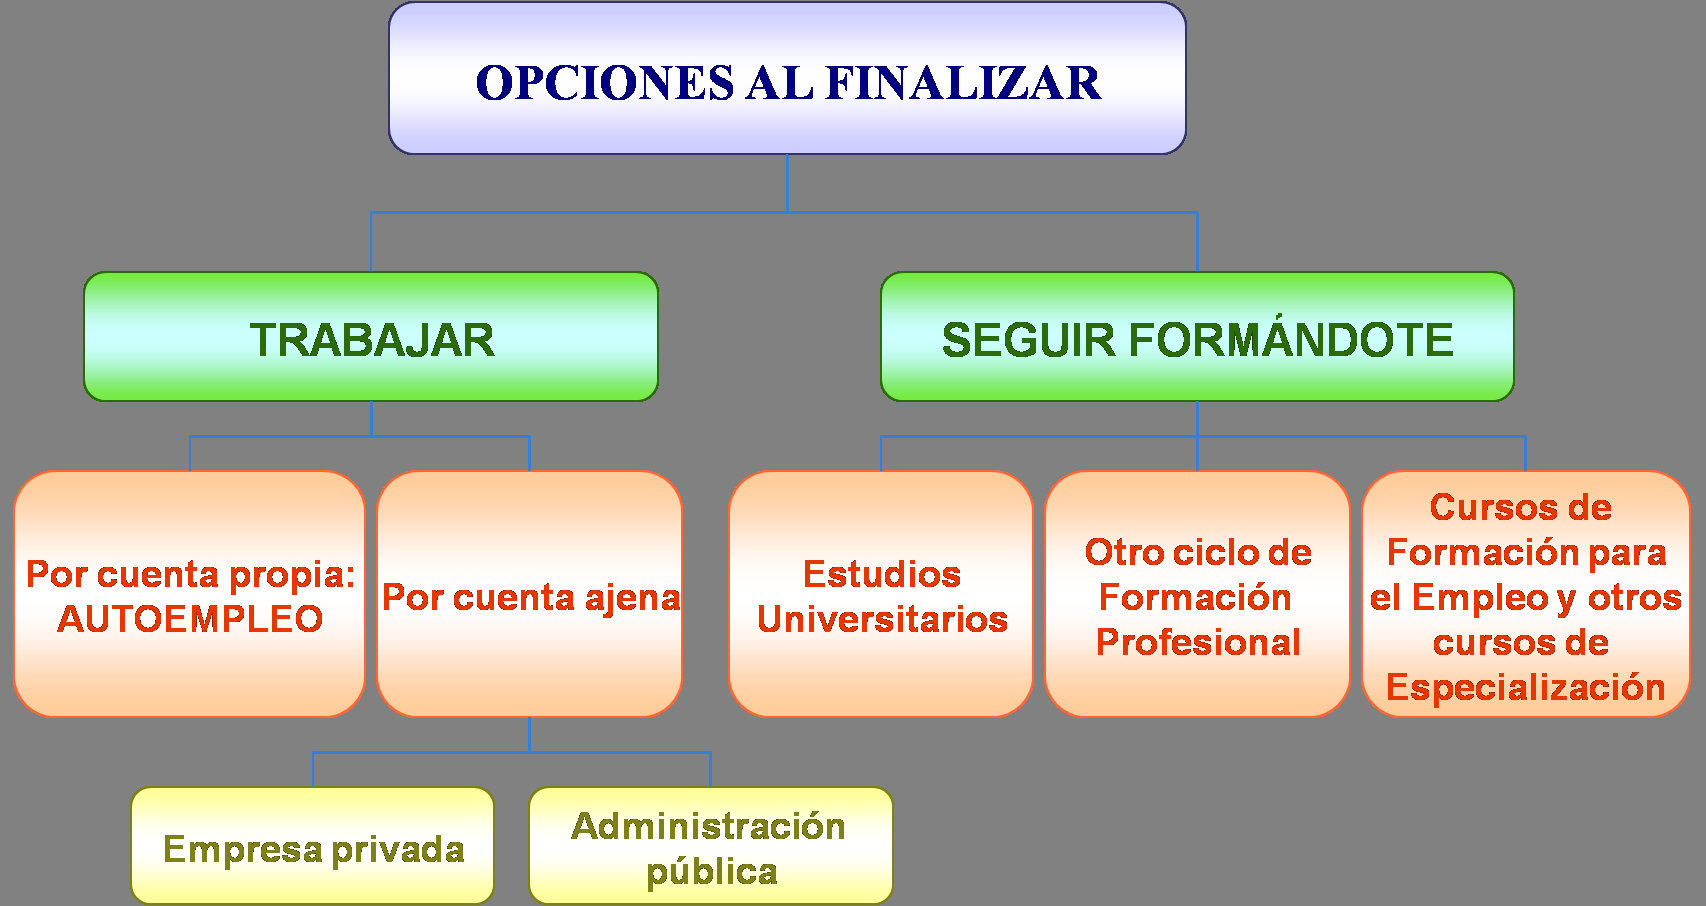
\includegraphics[scale=0.30]{esquema-FP.png}
    \caption{Salidas después de acabar un Ciclo Superior}
\end{figure}

Como vemos en el esquema hay muchas posibilidades tras acabar tus estudios. Puedes seguir formándote, ya sea haciendo otro módulo, accediendo a la universidad o realizando cursos de formación para el empleo. También puede lanzarte al mercado laboral, ya sea por cuenta propia o por cuenta ajena. Dependiendo de las opción que tomes, deberás informarte de sus requerimientos, algunos de los cuales no se logran de la noche a la mañana.

Por lo tanto, lo primero es fijarte unos objetivos, para lo que es necesario que conozcas el proceso de toma de decisiones, que veremos en el siguiente punto.

\section{La Toma de Decisiones}
La \textbf{toma de decisiones} es el \textbf{proceso} por el cuál se realiza \textbf{una elección} entre \textbf{las alternativas} para resolver diferentes situaciones de la vida. Consiste, básicamente, en elegir una alternativa de entre las disponibles a los efectos de resolver un problema.

Aunque no existe una receta infalible, antes de tomar una decisión que afecta a tu futuro es conveniente que analices todas las posibilidades.

\subsection{Fases de la Toma de Decisiones}
Dentro del proceso de toma de decisiones podemos diferenciar varias fases, las cuales son las siguientes:

\begin{itemize}
    \item \textbf{Reconocimiento}: la toma de decisiones comienza cuando se presenta una nueva situación de oportunidades o amenazas. Para que se pueda considerar una toma de decisiones debe haber al menos dos alternativas entre las que escoger.
    \item \textbf{Enumeración de las alternativas/opciones}: en esta etapa se definirán cuales son las alternativas y opciones, las cuales dependerán de tus metas y tus valores. Tener consciencia de tus prioridades y valores es muy importante y te ayudará a definir tus metas y alternativas. En esta fase ayuda hacer una lista con todas las opciones y alternativas.
    \item \textbf{Análisis/Evaluación de Alternativas}: en esta fase es necesario analizar las alternativas, usando la lista elaborada en el punto anterior, teniendo en cuenta las opciones que ofrece cada alternativa, así como sus ventajas he inconvenientes. Habrá también que analizar los recursos que requiere cada alternativa así como los beneficios esperados de está.

    Algo que nos puede ayudar es elaborar un cuadro con las diferentes alternativas y sus ventajas e inconvenientes como vemos en la siguiente figura.

    \begin{figure}[ht]
        \centering
        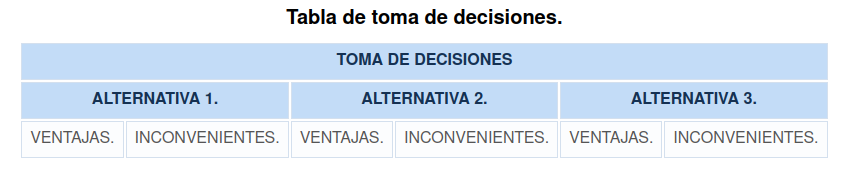
\includegraphics[scale=0.50]{tabla-decisiones.png}
        \caption{Alternativas del proceso de toma de decisiones}
    \end{figure}

    \item \textbf{Elección}: tras evaluar cada alternativa, hay que decantarse por una. Ahora deberás centrarte en ella y estudiar como ponerla en práctica, elaborando una estrategia, examinando de nuevo la información recogida sobre esta alternativa, sus posibles dificultades y como superarlas.
    \item \textbf{Ejecución}: en esta etapa se lleva a la práctica la alternativa elegida. Pueden surgir contratiempos menores, que harán vacilar, pero al final se puede llevar a cabo. En cambio, si se presentan desafíos o insatisfacciones más serías, puede abandonarse esta alternativa y volver al principio del proceso de toma de decisiones, con la ventaja de la experiencia ya ganada.
\end{itemize}

\section{¿Quieres Trabajar?}
En esta sección vamos a analizar las diferentes opciones que tenemos de empleo así como la importancia de la búsqueda activa, el currículum vitae o el proceso de selección, entre otras cosas.

\subsection{Búsqueda de Empleo: Factores de Ocupabilidad}
La búsqueda de empleo supone un gran trabajo, pero esta comprobado que las personas que se preparan una estrategia en su búsqueda de empleo aumenta su efectividad en una 70\% frente a las que no lo hacen. A la hora de elaborar una estrategia hay muchos factores que influyen en su eficacia, como la información que tengamos del mercado laboral, el nivel de formación y las posibilidades de mejorarlo, el grado de motivación y autoestima, las habilidades profesionales y personales, así como el dominio de determinadas técnicas y herramientas para la búsqueda de empleo.

Dos personas, con la misma formación y un experiencia profesional parecida pueden tener resultados muy distintos en el proceso de búsqueda de empleo. Esto se debe a que influyen una serie de factores que influyen en el proceso y que se conocen como factores de ocupabilidad.

Los \textbf{factores de ocupabilidad} son características que determinan tu forma de trabajar, de relacionarte con los demás y que las empresas consideran sumamente importantes. Parece demostrado que determinadas capacidades hacen que el rendimiento de un trabajador sea muy superior al de otro que tiene los mismos conocimientos técnicos pero que no posee estas capacidades.

Los factores de ocupabilidad se pueden clasificar en cuatro grupos \cite{trabyper}:

\begin{enumerate}
    \item \textbf{Factores estructurales}: estos factores tienen que ver con el mercado laboral al que se pretende acceder y es prácticamente imposible influir en ellos.
    \item \textbf{Factores personales}: en estos factores influyen tu experiencia y conocimiento, pero también tu edad, sexo, estado civil o algún tipo de problema físico que pueda afectar al desarrollo de tu actividad laboral.
    \item \textbf{Factores competenciales}: estos factores son los que tienen que ver con tus habilidades profesionales y es donde el entrevistador comparará tus habilidades técnicas con el resto de candidatos.
    \item \textbf{Factores psicosociales}: estos factores están influenciados por el entorno social y cultural e incluyen elementos como la disponibilidad hacia el empleo, madurez ocupacional, apoyo socio-familiar, autoimagen profesional y personal, etc...
\end{enumerate}

Por último, te proponemos realizar un cuestionario cuya finalidad es el análisis de las actitudes personales requeridas para el desempeño de un puesto de trabajo determinado. Este \href{https://www.ich.es/Empleabilidad/FactPsicoOcupa/FactPsicoOcupa.php}{cuestionario} te ayudará a conocer tus puntos débiles en este aspecto.

\subsection{El Proyecto Profesional}
El \textbf{proyecto profesional} es un documento donde identificaremos cuáles son nuestros objetivos profesionales y personales. El objetivo del mismo es evaluar tu formación, tu experiencia e identificar tus cualidades y capacidades para valorar si cumples los requisitos que el mercado laboral esta demandando en dicho momento.

Esto permite conocer de manera óptima tu personalidad y perfil profesional, orientándote en la búsqueda de empleo para seleccionar las ofertas que se ajusten a tus características.

El proyecto profesional consta de 3 fases con sus respectivos documentos, como vimos en la sección 1.4 \textit{``La Carrera Profesional''}, y que vamos a repasar en este punto. Así, las fases del proyecto profesional son las siguientes:

\begin{enumerate}
    \item \textbf{Mis aportaciones al mercado laboral (Balance Personal)}: debemos conocernos a nosotros mismos de forma que podamos vendernos a las empresas, destacando nuestra fortalezas y ``camuflando'' nuestras debilidades. Por lo que deberás hacer un listado con los aspectos positivos y negativos de tu personalidad.
    \item \textbf{Análisis del Mercado Laboral}: cuando nos decidamos por un determinado puesto de trabajo deberemos realizar una \textbf{prospección} del mercado laboral para saber cuales son los requisitos del puesto, así como que ofrecen las empresas. Una vez que hayamos recopilado la información, podemos hacer una tabla similar a la de la siguiente figura \ref{tab:emp} para ver si el puesto se ajusta a nuestro perfil profesional.

    \item \textbf{Objetivo Profesional}: una vez que conocemos lo que podemos ofrecer y lo que piden las empresas, tenemos que definir a que puestos vamos a optar, las condiciones laborales que estamos dispuestos a aceptar y elaboraremos un plan de acción para conseguir nuestro objetivo.
\end{enumerate}

\vspace{10ex}

\begin{figure}[ht]
    \centering
    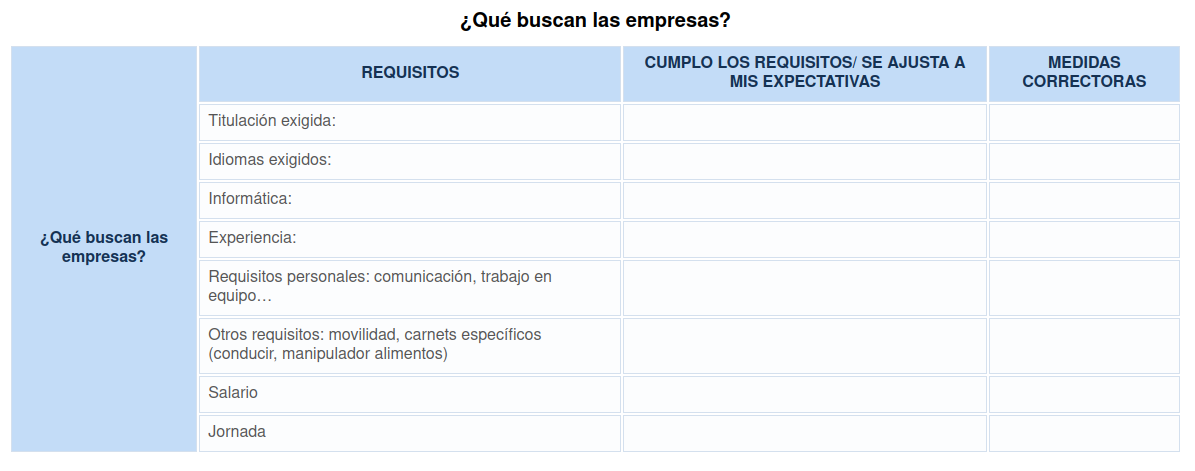
\includegraphics[scale=0.50]{tabla-empresas.png}
    \caption{Perfil profesional vs Requisitos empresas}
    \label{tab:emp}
\end{figure}

Es \textbf{importante} que consultes los siguientes modelos para ampliar la información dada en este punto y ver la estructura de un proyecto personal y un plan de empresa.

\begin{itemize}
    \item Modelo Proyecto Personal - \url{http://www.publicacions.ub.edu/liberweb/mundo_trabajo/cuestionario.pdf}
    \item Modelo Plan de Empresa - \url{https://blog.cofike.com/plan-de-empresa-ejemplo/}
\end{itemize}

También encontrar información sobre el proyecto personal con más detalle de todos los documentos implicados en cada fase en el \textbf{Anexo A.1}.

\subsection{El Proceso de Búsqueda de Empleo}
La búsqueda de empleo requiere de la utilización de un conjunto de técnicas las cuales se refieren al conocimiento, aprendizaje y mejora de todas aquellas estrategias y habilidades que enriquecen los recursos personales y aumentan la posibilidad de encontrar trabajo.

Estas técnicas no nos van a garantizar que encontremos trabajo inmediatamente pero si van a ayudar a aumentar nuestras posibilidades en la búsqueda de empleo.

La búsqueda de empleo implica llevar a cabo las siguientes acciones:

\begin{enumerate}
    \item \textbf{¿Que trabajo busco?} (Proyecto Profesional)
    \item \textbf{Localizar Ofertas} (Canales de búsqueda de empleo)
    \item \textbf{Contactar con las ofertas} (Instrumentos de presentación: carta y currículum)
    \item \textbf{Entrar en el proceso de selección} (Entrevista, Psicotécnicos,...)
    \item \textbf{Contratación} (modelos de contrato y derechos laborales)
\end{enumerate}

De la lista anterior ya hemos visto el proyecto profesional, por lo que en esta sección nos centraremos en las siguientes, salvo en los modelos de contrato y derechos laborales que se estudiarán con mas detalle en las siguientes unidades.

\subsubsection{Canales de Búsqueda de Empleo}
La búsqueda de empleo no es una tarea sencilla, y saber utilizar correctamente los diferentes canales de los que disponemos para realizarla puede facilitarnos un poco el proceso.

Podemos diferenciar dos tipos de \textbf{canales de búsqueda de empleo}, los pasivos y los activos.


\subsubsection*{Canales Pasivos}
Son canales en los que la búsqueda se deja en manos de terceros y se está a la espera de que te ofrezcan un puesto de trabajo. En este caso, entregarás un currículum o rellenarás una solicitud de empleo y se pondrán en contacto contigo cuando reciban ofertas que de adapten a tu perfil. Los principales medios de tipo de canales son:

\begin{itemize}
    \item \textbf{Agencias de Colocación Personal}: empresa destinada a poner en contacto a empresas que ofertan empleos con personas que los demanda. Puedes encontrar un directorio con una lista de consultorías y agencias de colocación en los siguientes enlaces:
    \begin{itemize}
        \item \href{https://www.infojobs.net/#seccion3}{Consultorías de Selección de Personal}
        \item \href{https://www.informacion-empresas.com/745_SELECCION-COLOCACION-PERSONAL.html}{Directorio de empresas de colocación y selección}
    \end{itemize}
    \item \textbf{Empresas de Trabajo Temporal} (ETTs): empresa que se encarga de poner a disposición de otra empresa, con carácter temporal, trabajadores que ha contratado. En el siguiente enlace puedes ver una lista del Ministerio de Trabajo con las principales ETTs.
    \begin{itemize}
        \item \href{https://expinterweb.mites.gob.es/sigett/consultaPublicaETT}{Lista de Empresas de Trabajo Temporal}
    \end{itemize}
    \item \textbf{Asociación de Técnicos de Informática}: esta asociación puede ser una vía para informarte sobre el empleo en tu campo profesional, así como acceder a su bolsa de trabajo, cursos, etc...
    \begin{itemize}
        \item \href{https://www.ati.es/}{Asociación de Técnicos de Informática}
    \end{itemize}
    \item \textbf{Bolsa de trabajo del centro en el que estudias}: muchos de los IES donde se imparten enseñanzas de formación profesional cuentan con bolsas de trabajo relacionadas con los Ciclos Formativos que imparten.
    \item \textbf{Sindicatos}, \textbf{Ayuntamientos} y otras \textbf{entidades públicas} con servicios de orientación al empleo.
    \item \textbf{Servicio Público Estatal de Empleo} (SEPE) o \textbf{servicios de colocación} de tu \textbf{Comunidad Autónoma}.
    \item \textbf{Internet}: hay un montón de páginas web dedicadas a la búsqueda de empleo, que te permiten crearte un currículum o formulario para mandarte ofertas que se adapten a tu perfil. Algunas de las más conocidas son las siguientes:
    \begin{itemize}
        \item \href{https://www.infojobs.net/}{Infojobs}
        \item \href{https://www.trabajos.com/}{Trabajos.com}
        \item \href{https://www.infoempleo.com/}{Infoempleo}
        \item \href{https://www.primerempleo.com/}{PrimerEmpleo}
        \item \href{https://www.oficinaempleo.com/}{OficinaEmpleo}
        \item \href{https://www.opcionempleo.com/}{OpciónEmpleo}
    \end{itemize}
\end{itemize}

Además de estos podemos encontrar multitud de plataformas especializadas en sectores concretos o en modos de trabajo concreto, como búsqueda de empleo para trabajar en remoto, para freelancers, trabajar en el extranjero, etc...

\subsubsection*{Canales Activos}
A diferencia de los canales pasivos, donde se requiere poca activad, en los canales activos se exige que haya más participación, debiendo intervenir en la búsqueda y selección de las ofertas de empleo, envío de currículum vitae, comunicación con familiares y amigos, etc... Los principales canales activos, son los siguientes:

\begin{itemize}
    \item \textbf{Red de Contactos Personal}: se considera que el 60\% de las ofertas de empleo no llegan a publicarse, ya que las empresas primero buscan entre sus conocidos. Esto pone de relieve la importancia de crearse una red de contactos que puedan ayudarte a encontrar empleo.
    \item \textbf{Autocandidatura o mailing}: es una variedad del marketing directo que consiste en enviar tu currículum a empresas que puedan necesitar trabajadores con tu perfil profesional. Para ello deberes buscar los datos de la empresa y enviarle tu currículo y carta de presentación a la persona responsable de las contrataciones. Suele hacerse por email.
    \item \textbf{Webs especializadas en empleo}: además de las comentadas en los canales pasivos, hay algunas webs en las que es recomendable visitarlas todos los días y consultar las ofertas que van apareciendo.
    \item \textbf{SEPE: Punto de Encuentro de Empleo}: en la web del servicio público de empleo podrás consultar las ofertas de trabajo que hay en tu provincia. En este \href{https://www.empleate.gob.es/empleo/#/trabajo?search=*&pag=0}{enlace} puedes acceder directamente al Punto de Encuentro del SEPE.
    \item \textbf{Televisión}: existen programas de televisión destinados al empleo, donde diariamente se exponen ofertas de trabajo. Uno de ellos es el programa de la 2 de TVE, \textit{``Aquí hay trabajo''}.
    \item \textbf{Prensa, radio, teletexto}: en estos medios de comunicación podrás encontrar ofertas de trabajo a las que podrás remitir tu currículum. Los domingos, especialmente, se publican suplementos sobre empleo en muchos periódicos de tirada nacional y local.
    \item \textbf{Empleo para Discapacitados}: por último, ONCE a través de su fundación FSC Inserta ofrece servicios de inserción laboral para discapacitados. No dudes en visitar su \href{https://www.insertaempleo.es/}{su página web} si tienes alguna discapacidad.
\end{itemize}

\subsubsection{Instrumentos de Presentación: Carta y Currículum}
Ahora ya tenemos claro cual es nuestro perfil laboral, hemos creado un proyecto profesional con nuestras metas y seleccionado los puestos a los que queremos optar. Además conocemos los diferentes canales donde podemos buscar empleo.

El siguiente paso es conocer dos instrumentos que nos vendrán muy bien a la hora de promocionarnos y ``vendernos'' a las empresas: \textbf{la carta de presentación} y \textbf{el currículum vitae}. Estos documentos nos precederán en cualquier empresa en la que queramos trabajar y nos servirán para diferenciarnos de nuestro competidores, aunque su principal función es \textbf{conseguirnos una entrevista} de trabajo. Por ello, deben estar redactados ajustados a las exigencias del puesto de trabajo al que quieres optar y que muestre una imagen de ti atractiva para el empleador.

\subsubsection*{La Carta de Presentación}
La \textbf{carta de presentación} se envía a aquellas empresas o lugares que pueden ofrecer oportunidades de empleo, es la ``tarjeta de visita'' que acompaña a tu currículum vitae. Su objetivo es atraer la atención de la persona que la lea, pensar que tienes un perfil perfecto para cubrir el puesto que se ofrece y animar a la lectura de tu currículum.

Las cartas de presentación de clasifican en dos tipos:

\begin{itemize}
    \item \textbf{Carta de Respuesta a una Oferta de Empleo}: esta se envía como respuesta a alguna oferta de empleo en algún medio e irá acompañando a tu currículum. Debe aludir necesariamente al anuncio en cuestión, señalando su referencia. En ella debes destacar por qué es interesante tu candidatura.
    \item \textbf{Carta de Autocandidatura}: carta que se envía por iniciativa propia a una empresa que pueda necesitar profesionales con nuestro perfil, ya sea en ese momento o en un futuro cercano. Debe explicar que te ha motivado a acercarte a la empresa y que puedes aportar. Si es interesante las empresas pueden archivarla y tenerla en cuenta en próximos procesos de selección.
\end{itemize}

Hay que tener un par de aspectos en cuenta antes de lanzarte a redactar la carta de presentación:

\begin{itemize}
    \item \textbf{Infórmate} sobre la \textbf{empresa} a la que te diriges y el \textbf{puesto} al que quieres optar. Identifica la cultura corporativa y resume los elementos claves del perfil.
    \item Intenta \textbf{averiguar} quien \textbf{realiza la selección de personal} y cual es su nombre. Así podrás dirigir la carta a esa persona concreta aumentando la probabilidad de ser leída.
\end{itemize}

En los siguientes enlaces puedes consultar diferentes modelos de carta de carta de presentación así como un resumen de lo que hemos visto sobre ella.

\begin{itemize}
    \item \href{https://www.modelocurriculum.net/modelos-carta-presentacion.html}{Modelos de Carta de Presentación}
    \item \href{https://www.mites.gob.es/es/mundo/consejerias/eeuu/webempleo/es/encontrar-empleo/cartapresentacion/index.htm}{Estructura básica de una Carta de Presentación}
\end{itemize}

\subsubsection*{El Currículum Vitae}
El currículum vitae es un historial profesional, donde deben figurar todos los datos académicos y experiencia de una persona a lo largo de su vida. Debe presentar tu candidatura como la mas idónea, de forma que el empleador muestre interés por tí.

Existen varios tipos de currículum:

\begin{itemize}
    \item Cronológico
    \item Cronológico inverso
    \item Funcional
\end{itemize}

Deberás escoger el que mejor se ajuste a tu perfil, aunque en los últimos tiempos se esta imponiendo el cronológico inverso. En la página \href{https://www.modelocurriculum.net/tipos-de-curriculum.html}{modelocurriculum.net} podrás encontrar mas información sobre los modelos de currículum que existen cuales son las tendencias.

Algunas empresas están empezando a solicitar videocurrículum digital. Consiste en la grabación de un breve vídeo, donde el candidato/a se dan a conocer, explicando por qué están buscando trabajo, su formación, su experiencia, etc...

Por todo esto, es importante que consultes el \textbf{Anexo A.2}, para aprender bien los tipos de currículum que existen y cual es su estructura, para elaborarlos correctamente.

\subsubsection{La Entrevista de Selección}
Los instrumentos que hemos visto hasta ahora en esta unidad tienen como fin último proporcionarte una entrevista de trabajo. Es el punto culminante del proceso y también el mas subjetivo.

Desde el punto de vista de una empresa, \textbf{los objetivos} de una entrevista de trabajo son:

\begin{itemize}
    \item Evaluar la idoneidad de una candidatura para el puesto ofertado. Se trata de averiguar si tienes las aptitudes y experiencia necesaria para aportar una contribución provechosa a la empresa.
    \item Comprobar que encajas en la empresa, según tu personalidad, temperamento y habilidades sociales.
    \item Obtener información que permita comparar tus puntos débiles y fuertes con los de otros candidatos.
\end{itemize}

Desde tu punto de vista, el \textbf{objetivo} de la entrevista es \textbf{conseguirte un empleo} y demostrar que tu candidatura es la mejor, además la entrevista puede servirte para comprobar tu compatibilidad con el empleador potencial y su empresa.

Para prepararse bien una entrevista e incrementar la posibilidades de éxito hay que tener en cuenta las diferentes fases que tiene y como debemos prepararnos en cada uno, así como que esperar de ellas. En la siguientes figura puedes ver una tabla con las fases de una entrevista de selección y algunos consejos que incrementarán nuestras posibilidades de superarla.

\begin{figure}[ht]
    \centering
    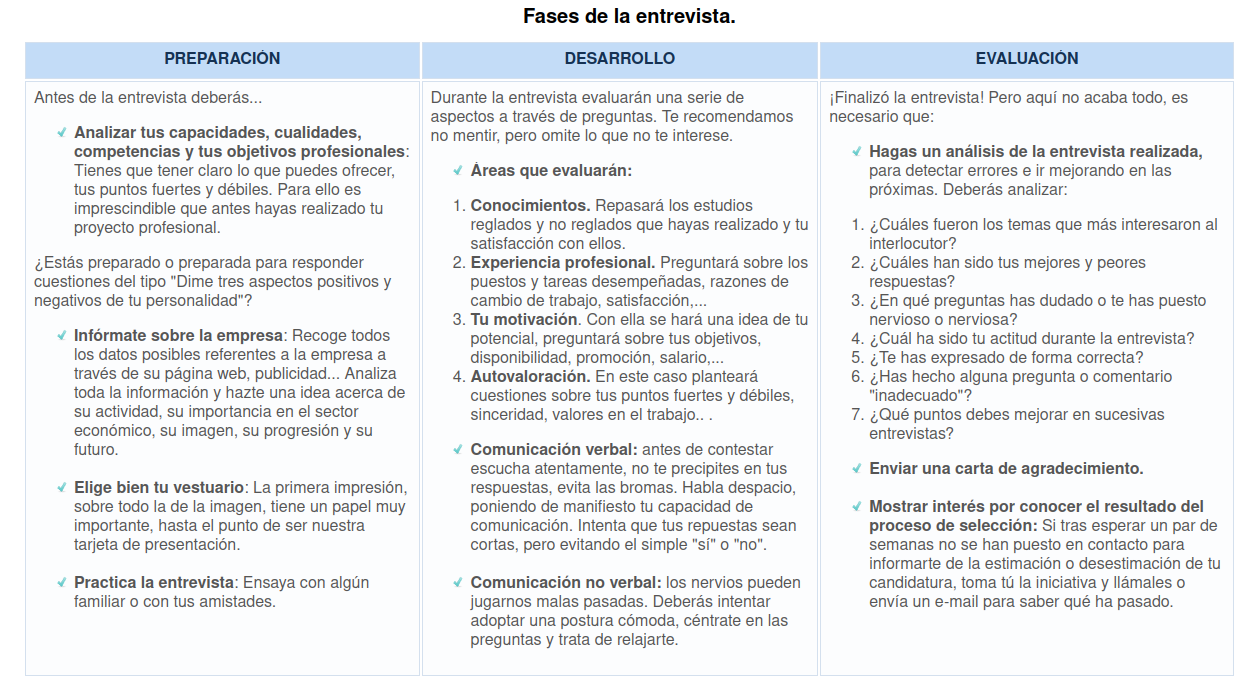
\includegraphics[scale=0.45]{fases-entrevista.png}
    \caption{Fases de una entrevista de selección}
\end{figure}

Ahora que ya tienes una idea sobre que es una entrevista de selección y cuales son sus fases, te recomendaríamos que practicaras con algún familiar o amigo estás entrevistas para que te vayas acostumbrando y afrontes una real con mayor tranquilidad.

\subsubsection{Pruebas de Selección}
Además de la entrevista de selección, la empresas pueden utilizar \textbf{pruebas de selección} en sus procesos de selección. Éstas pueden ser posteriores o anteriores a la entrevista de selección.

La finalidad de estas pruebas es medir una serie de características personales, conductuales o profesionales de los candidatos para determinar la adecuación al puesto de trabajo. Con ellas se obtiene información de las competencias, capacidades, inteligencia, habilidades, conductas, rasgos de personalidad, etc...

Las pruebas pueden ser de diferente índole, como escritas, test de desarrollo práctico-profesional, técnicas de simulación de situaciones, etc..

Los tipos mas comunes que nos podemos encontrar son los siguientes:

\begin{itemize}
    \item \textbf{Test de Proyectos}: buscan predecir el comportamiento futuro de una persona. Tratan de revelar los aspectos más escondidos de la personalidad de un candidato, como mal control de sus emociones, falta de iniciativa, excesiva ambición,..
    \item \textbf{Test de Aptitudes}: valoran los requisitos específicos del candidato/a para un determinado puesto de trabajo. Este test trata de medir diferentes funciones como el tiempo de reacción, la coordinación...
    \item \textbf{Test de Inteligencia}: valoran el nivel intelectual así como diferentes factores relacionados con la inteligencia. Es usual someter al candidato/a a una batería de preguntas contra el tiempo, donde se le pide hacer secuencias lógicas o escribir una serie de palabras por minuto.
    \item \textbf{Test de Personalidad}: miden características personales del candidato como autocontrol, emocionalidad, iniciativa,... Se le pregunta que responda a una serie de preguntas, bien diciendo si o no, o dando una respuesta libre espontánea.
    \item \textbf{Pruebas Profesionales}: sirven para estudiar las competencias del candidato relacionadas con el puesto de trabajo.
    \item \textbf{Pruebas Físicas y Médicas}: se utilizan para determinar el estado físico y de salud del candidato.
    \item \textbf{Dinámicas de Grupo}: consiste en exponer a los candidatos/as ante diferentes situaciones para que interactúen entre ellos, evaluando la capacidad de comunicación, de liderazgo, el rol que asume una persona dentro de grupo, etc..
\end{itemize}

Por último, cabe destacar, que en el sector de las nuevas tecnológicas, especialmente para los \textbf{puestos} relacionados con el \textbf{desarrollo de software}, casi siempre nos encontraremos con \textbf{pruebas técnicas}, donde nos propondrán la realización de un ejercicio de software para ver como lo resolvemos y si tenemos los conocimientos necesarios para cubrir el puesto.

\subsection{Trabajar en Europa}
La \textbf{libre circulación de trabajadores} es uno de los principios fundamentales de la Unión Europea. Esto significa que cualquier ciudadano de la UE puede trabajar en cualquiera de los estados miembros en igualdad de condiciones, con los mismos derechos y obligaciones independientemente de cuál sea su país de origen.

Si tienes interés en trabajar en Europa al acabar el Ciclo Formativo, es importante que conozcas los recursos de internet que la Unión Europea pone a disposición de sus ciudadanos para facilitar esta tarea.

\begin{itemize}
    \item \textbf{EURES: Portal Europeo de la Movilidad Profesional}: este portal tiene como objetivo servir de enlace entre los distintos servicios públicos de empleo de la UE. A través de su página web puedes acceder a una base de datos común con ofertas de empleo y convocatorias en toda la UE. Puedes visitar la plataforma EURES en este enlace:
    \begin{itemize}
        \item \href{https://eures.ec.europa.eu/index_es}{Plataforma EURES}.
    \end{itemize}

    Desde la web también se puede acceder a aspectos prácticos sobre el trabajo y la vida en los diferentes países, como características del mercado laboral, legislación, etc...

    \vspace{5ex}

    \item \textbf{Tu Europa}: esta página de la Comisión Europea ofrece información útil sobre cualquier país de la Unión Europa: fiscalidad,  derechos, seguridad social, trámites, reconocimiento de titulaciones...
    datos común con ofertas de empleo y convocatorias en toda la UE. Puedes visitar la plataforma EURES en este enlace:
    \begin{itemize}
        \item \href{https://ec.europa.eu/youreurope/citizens/index_es.htm}{Tu Europa}.
    \end{itemize}

    \item \textbf{Portal Europeo de la Juventud}: el objetivo de este portal es promover el trabajo, la ciudadanía activa y la solidaridad entre los jóvenes de la UE. Podrás encontrar información relativa al trabajo, voluntariado, intercambio,... entre los jóvenes de la UE.
        \begin{itemize}
        \item \href{https://youth.europa.eu/go-abroad/working_es}{Portal Europeo de la Juventud}.
    \end{itemize}

    Si pinchas en el menú de la izquierda, \textbf{Trabajar}, accederás a un directorio con páginas web relacionadas con el trabajo.
\end{itemize}

Por último, hay que recordar que deberás utilizar el \textbf{modelo de currículum europeo} cuando encuentres una oferta a la que quieras presentarte. Este currículum podrás encontrarlo en la página de \href{https://europa.eu/europass/es/create-europass-cv}{Europass}, plataforma que contiene un dossier de documentos cuyo objetivo es facilitar la movilidad de trabajadores en los países miembros de la UE.

\subsection{Trabajar en la Administración Pública}
Ya sabes que una de las formas de trabajar es en la Administración Pública. Si es el camino que has decido tomar, es conveniente tener alguna información y conocer algunos recursos básicos para facilitar la tarea.

Aproximadamente un 15\% de la población activa trabaja para diferentes administraciones publicas españolas: Comunidades Autónomas, Ayuntamientos, Estado Central,.. Trabajar en la administración tiene sus ventajas, pero también sus inconvenientes, como podemos ver en la siguiente figura.

\begin{figure}[ht]
    \centering
    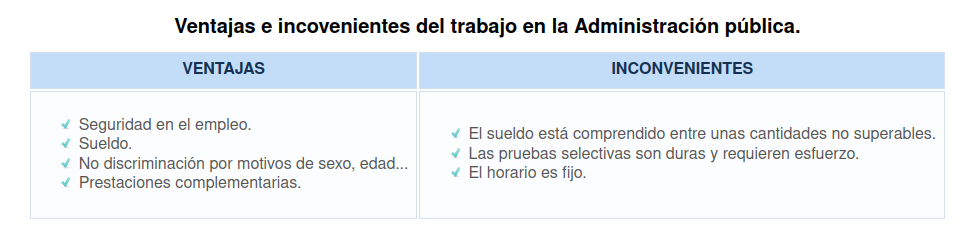
\includegraphics[scale=0.60]{ventajas-funcionario.png}
    \caption{Ventajas e Inconvenientes de trabajar con la Administración Pública}
\end{figure}

Aprobar una oposición no es fácil. No basta con estudiar y practicas sino que hay que tener una gran fuerza de voluntad para no desanimarse. Es imprescindible que sepas que puestos ofrece el ámbito público, cual es el temario, que tipo de pruebas se llevarán a cabo, o cuales son los \textbf{méritos baremables} en el caso de que sea un concurso de oposición público, entre otras cosas. Para ello deberás deberás realizar una primera labor de búsqueda de información, para ello, vamos a refrescar las salidas profesionales del ámbito público que ya hemos visto anteriormente en esta unidad.

Como recordarás, en el ámbito público tienes acceso a los puestos de \textbf{Técnicos Auxiliares Informáticos} de la Administración del Estado o las Autonómicas. Es aconsejable que busques diferentes oposiciones que te interesen y analices cual es el temario, los tipos de pruebas, que méritos son baremables y la creación de bolsas de trabajo.

Para informarte de que oposiciones se convocan y otra información referente a este tema puede consultar alguno de los siguientes enlaces:

\begin{itemize}
    \item \href{https://administracion.gob.es/pag_Home/empleoPublico/boletin.html}{Boletín Semanal de Empleo Público}
    \item \href{https://www.empleopublico.net/}{Empleopublico.net}
    \item \href{https://www.oposiciones.net/}{Oposiones.net}
    \item \href{https://www.juntadeandalucia.es/institutodeadministracionpublica/institutodeadministracionpublica/publico/home.filter?idsitio=15}{Instituto Andaluz de Administraciones Públicas}
\end{itemize}

Por último, recordarte que en el \textbf{Anexo A.3} encontrarás información mas detallada sobre los diferentes tipos de relaciones laborales que se pueden entablar con la Administración Pública.

\section{Seguir Formándose: Importancia de la Formación Permanente}
La motivación y la formación son cuestiones clave que se deben abordar desde una perspectiva contextualizada en la sociedad actual. El mercado laboral cambiante y las nuevas necesidades hacen que \textbf{clave} una permanente \textbf{actualización de los conocimientos} y formación, ya que de otra forma estos quedarán obsoletos de forma rápida.

Tantos los cursos pequeños ligados a las TIC, hasta los cursos específicos relacionados con oficios o la profesión a ejercer nos sitúan mejor posicionados para afrontar las oportunidades que se nos presenten. Por ello, vamos a analizar las diferentes opciones formativas que podemos encontrarnos tras acabar un Ciclo Formativo, sin olvidar que hay que \textbf{estar continuamente formándose} para actualizar los conocimientos y ser competitivo.

\subsection{Estudios Universitarios}
Aunque la finalidad de la Formación Profesional Específica es formar profesionales preparados para su incorporación al mercado laboral, los titulados en Ciclos de Formación de Grado Superior pueden cursar otros estudios superiores como son los universitarios. En este aspecto, el \textbf{título de Técnico Superior} ofrece acceso directo a la universidad. En función del título que se haya cursado, se podrá acceder a unos u otros estudios universitarios.

En concreto, los Ciclos Formativos de \textbf{DAM},\textbf{DAW} y \textbf{ASIR}, permiten el \textbf{acceso} de diferentes \textbf{titulaciones de informática}, como el Grado en Ingeniería Informática, Grado en Ingeniería Informática del Software, Grado en Ingeniería Informática de Servicios y Aplicaciones, etc...

En lo referente al \textbf{acceso}, el \href{https://www.boe.es/diario\_boe/txt.php?id=BOE-A-2014-6008}{Real Decreto 412/2014} establece toda la normativa básica de los procedimientos de admisión a las enseñanzas oficiales de Grado y los procedimientos de admisión en las universidades públicas españolas.

También hay que recordar que al acceder a estudios universitarios desde un Ciclo Formativo Superior \textbf{sistema de convalidaciones}, que establece:

\begin{enumerate}
    \item Las convalidaciones entre quienes posean el título de Técnico Superior, y cursen enseñanzas universitarias de grado relacionadas con dicho título, serán de al menos, 30 créditos ECTS.
    \item Siempre que las enseñanzas universitarias de grado incluyan prácticas externas en empresas de similar naturaleza a las realizadas en los ciclos formativos, se podrán convalidar, además, los créditos asignados al módulo profesional de Formación en Centros de Trabajo del título de Técnico Superior relacionado con dichas enseñanzas universitarias.
    \item Se podrán también convalidar otros créditos teniendo en cuenta la adecuación entre las competencias y conocimientos asociados a materias conducentes a la obtención de títulos de grado, o equivalente, con créditos obtenidos en los módulos profesionales superados del correspondiente título de Técnico Superior.
\end{enumerate}

\subsection{Estudiar otro Ciclo Formativo}
Otra posibilidad es estudiar ciclos formativos relativos a la familia que ya hemos estudiado, ya que nos permiten adquirir otra especialidad con relativa facilidad, al tratarse de estudios con contenidos similares, pudiendo convalidar las asignaturas comunes entres los diferentes Ciclos Formativos.

En nuestro caso, las titulaciones que entran dentro de este grupo son las que hemos visto durante este tema, \textbf{Técnico Superior en Desarrollo de Aplicaciones Multiplataforma}, \textbf{Técnico Superior en Desarrollo de Aplicaciones Web} y \textbf{Técnico Superior en Administración de Sistemas Informáticos en Red}.

\subsection{Formación Profesional para el Empleo}
La \textbf{Formación para el empleo} es el conjunto de instrumentos y acciones que tienen por objeto impulsar y extender entre las empresas y los trabajadores ocupados y desempleados una formación que responda a sus necesidad. Esta formación se integra dentro del Sistema de Formación Profesional, al igual que la Formación Inicial, constituida por los ciclos formativos de grado medio y superior del Sistema Educativo.

La Formación Profesional para el Empleo se articula en cursos o acciones formativas integradas en Familias Profesionales y esta dirigida a \textbf{trabajadores}, ya estén ocupados o desempleados, de deseen cualificarse, re-cualificarse o especializarse para mejorar sus oportunidades de acceso o permanencia en el mercado laboral.

Existe una extensa oferta formativa, tanto en modalidad presencial, como a distancia, mixta y teleformación. Los cursos suelen tener una duración variables, si bien los mas extensos no superan el año de duración. Ademas, estos cursos están financiados/subvencionados por las Administraciones Públicas, siendo la mayoría de ellos gratuitos.

Estos cursos \textbf{son ofertados} por las \textbf{Administraciones Públicas}, \textbf{Sindicatos}, \textbf{Organizaciones Empresariales} y \textbf{Centros} de formación \textbf{privados}. En el caso de asociaciones empresariales y sindicatos no es necesario estar afiliado, ya que estos cursos se financian en parte con las cuotas de todos los trabajadores.

Los \textbf{cursos de especialización} son otra opción, concretamente en la familia de informática podemos encontrar los siguientes:

\begin{itemize}
    \item \href{https://www.todofp.es/que-estudiar/loe/informatica-comunicaciones/ce-inteligencia-artificial-bigdata.html}{Curso de Especialización en Inteligencia Artificial y Big Data}
    \item \href{https://www.todofp.es/que-estudiar/loe/informatica-comunicaciones/ce-desarrollo-videojuegos-realidad-virtual.html}{Curso de Especialización en Desarrollo de Videojuegos y Realidad Virtual}
    \item \href{https://www.todofp.es/que-estudiar/loe/informatica-comunicaciones/ciberseguridad-entornos-tecnologias-informacion.html}{Curso de Especialización en Ciberseguridad en Entornos de las Tecnologías de la Información}
\end{itemize}

Además de los cursos de formación para el empleo, las \textbf{entidades privadas ofertan cursos} que pueden ayudarte a especializarte y profundizar en las áreas que más te interesen. Para saber que centros imparten un curso determinado, solo tienes que buscar el curso en cualquier buscador de internet y te aparecerán muchos resultados.

\subsection{Estudiar en Europa}
Cada vez son más los alumnos que deciden estudiar o realizar la prácticas de Formación en Centros de Trabajo en otro país europeo. Esto te permitirá adquirir nuevas competencias lingüísticas, así como conocer otra cultura y hacer amigos de diferentes países. Además, es positivo para tu currículum.

A continuación listamos un conjunto de recursos web que te serán de gran utilidad si te has decidido por esta opción:

\begin{itemize}
    \item \textbf{\href{https://spain.representation.ec.europa.eu/index_es}{PLOTEUS}} (Portal on Learning Opportunities Throughout the European Space): este portal contiene información sobre las oportunidades de aprendizaje en el espacio europeo. Tiene como objetivo ayudar a estudiantes, trabajadores, padres, orientadores y profesores a encontrar información sobre las opciones de aprendizaje a lo largo de la vida en Europa. Se estructura en la siguientes secciones:
    \begin{itemize}
        \item \textbf{Oportunidades de Aprendizaje y Posibilidades de Formación}: contiene múltiples enlaces a páginas web de universidades e instituciones de enseñanza superior, bases de datos de centros escolares y formación profesional, así como cursos de enseñanza para adultos.
        \item \textbf{Sistemas de Educación y Formación}: contiene información sobre los distintos sistemas de enseñanza y formación de los países europeos.
        \item \textbf{Programas de Intercambio y Becas}: contiene información sobre todas las becas y programas de intercambio que podemos solicitar, entre los que se encuentran los programas ERASMUS, Leonardo da Vinci, Sócrates y Tempus entre otros.
        \item \textbf{Vivir en el Extranjero}: sección con información sobre todo lo que debes saber cuando te trasladas a otro país de la UE, como coste de vida, gastos de educación, alojamiento, marco legal, y otra información general sobre los países europeos.
    \end{itemize}
    \item \textbf{\href{https://www.estudiareneuropa.eu/}{Estudiar en Europa}}: en esta página se ofrece información sobre cursos y programas, estudios superiores, así como toda la información que necesitas conocer para iniciar tu aventura europea.
    \item \textbf{\href{https://youth.europa.eu/home_es}{Portal Europeo de Juventur}}: en esta plataforma se recogen todas las oportunidades y posibilidades para estudiar en Europa, especialmente enfocada a la gente joven.
\end{itemize}

Entre todas estas opciones, cabe destacar el \textbf{Programa Erasmus}, uno de los más conocidos y que permite la realización de una parte de las prácticas de FTC en otro país europeo. Para más información, consulta con tu centro de estudios.

\chapter{La Relación Colectiva en el Trabajo}

\chapter{La Seguridad Social}
La \textbf{Seguridad Social} es una creación de finales del s. XIX. Con anterioridad, los riesgos que esta cubre eran cubiertos por diversos mecanismos, tales como el ahorro individual, la caridad, la beneficencia, los seguros privados, etc. La moderna S.S aparece en la \textbf{Alemania de Bismarck} al instituirse los seguros obligatorios de enfermedad (1883), accidente de trabajo (1884), vejez e invalidez (1889, para los trabajadores de la industria.

En nuestro país, la evolución histórica de la S.S podemos fecharla en 1919, año en el que aparece el primer seguro obligatorio de jubilación, denominado \textbf{Retiro Obrero}. Pero no será hasta finales de la Guerra Civil española (1939), cuando aparezcan los \textbf{seguros obligatorios} de vejez, invalidez, muerte enfermedad, accidentes, desempleo y protección de la familia.

En este tema, vamos a ver en que consiste la seguridad social, cuales son sus características y toda la normativa relacionada con esta en España.

\section{Concepto y Normas Reguladoras}
En el transcurso de su vida, lo seres humanos están expuestos a una serie de \textbf{riesgos sociales}. Esto se produce principalmente por dos razones:

\begin{enumerate}
    \item Son riesgos que amenazan a a cualquier persona porque \textbf{son inherentes} a la propia vida del hombre en sociedad.
    \item Existe el convencimiento de que es la \textbf{propia sociedad} la que debe \textbf{organizar la prevención} y \textbf{reparación} de los daños derivados de estos riesgos o \textbf{contingencias comunes} y \textbf{profesionales}.
\end{enumerate}

Ante este problema ineludible y que afecta a la mayoría de la población, el Estado, dentro de su política de bienestar, articula el actual \textbf{Sistema de la Seguridad Social} constituido por un conjunto de de técnicas específicas de previsión, a través de las cuales se \textbf{garantiza} a los sujetos incluidos en su campo de aplicación la \textbf{asistencia} y \textbf{protección} adecuada ante determinados estados de necesidad derivados de las \textbf{contingencias} y \textbf{riesgos sociales} asegurados.

Los \textbf{grandes principios} que orientan la evolución de nuestro \textbf{Sistema de Seguridad Social} son:

\begin{itemize}
    \item \textbf{Contributividad}: se dice que estamos ante un sistema contributivo porque existe una proporción entre los percibido (prestaciones) y lo aportado mediante cotizaciones de empresarios y trabajadores que representa su principal fuente de financiación, siendo mucho menos la aportación del estado.

    \item \textbf{Universalidad}: se pretende alcanzar la máxima extensión en su acción protectora y campo de aplicación.

    \item \textbf{Solidaridad Intergeneracional}: mientras trabajamos, se contribuye a financiar las pensiones actuales.

    \item \textbf{Equidad e Igualdad de Derechos}: la acción protectora es independiente del momento o lugar de residencia del asegurado.

    \item \textbf{Suficiencia}: se intenta garantizar los niveles de bienestar mediante prestaciones adecuadas.

    \item \textbf{Unidad de Caja}: es Estado es el único titular de todos los recursos de la Seguridad Social.
\end{itemize}

Al margen de estos principios, la \textbf{Seguridad Social} esta regulada por diferentes \textbf{normas}, que dejando de lado el Derecho Comunitario Europeo, son las siguientes ordenadas \textbf{jerárquicamente}:

\begin{enumerate}
    \item La Constitución Española de 1978.
    \item La Ley General de la Seguridad Social, texto refundido aprobado por RDL 8/2015 (en adelante \textbf{LGSS}).
    \item Reglamentos generales y particulares de cada prestación.
\end{enumerate}

Durante este tema, veremos con más detalle estás normas y cuales son sus principales características, así como las diferentes prestaciones que ofrecen, pero primero en el siguiente punto, veremos cual es el campo de aplicación de la Seguridad Social.

\section{Campo de Aplicación}
En España la \textbf{asistencia sanitaria}  es \textbf{universal}, lo que significa que tendrán acceso a ella todas las personas que residan en nuestro país sin importar nacionalidad ni capacidad económica. En la mayoría de países desarrollados la asistencia sanitaria es universal, aunque hay excepciones como Estados Unidos, que es el único país industrializado sin un sistema generalizado  de asistencia sanitaria.

En nuestro país, el \textbf{campo de aplicación} de la Seguridad Social se delimita con arreglo a los \textbf{principios de territorialidad y nacionalidad}, con bases a los que quedan \textbf{incluidas} las siguientes \textbf{personas}:

\begin{enumerate}
    \item Los \textbf{españoles} que \textbf{residan} y \textbf{ejerzan}  normalmente su \textbf{actividad} en territorio nacional, ya sea como trabajadores por cuenta ajena, por cuenta propia, estudiantes y funcionarios públicos, civiles y militares, tendrán derecho a prestaciones contributivas si reúnen los requisitos legales. También los españoles residentes que \textbf{no desarrollen actividad alguna} tendrán derecho a \textbf{prestaciones no contributivas} si reúnen los requisitos legales.

    \item Los \textbf{españoles no residentes} cuando así lo establezca el Gobierno, como funcionarios de organizaciones internacionales y personal del servicio de la administración española en el extranjero.

    \item En cuanto a los \textbf{extranjeros} cabe distinguir los siguientes \textbf{supuestos}:
    \begin{itemize}
        \item Los hispanoamericanos, brasileños, andorranos y filipinos con residencia legal en España, quedan equiparados a los españoles.
        \item Los trabajadores comunitarios de la Unión Europea se equiparan a los nacionales, en virtud del principio de igualdad de trato que rige la normativa comunitaria (artículo 53 del tratado de la CEE).
        \item Los restantes extranjeros que residan legalmente en nuestro país, se someterán a lo dispuesto en los convenios suscritos a tal efecto, o a cuanto les fuera aplicable en virtud del principio de reciprocidad, es decir, que recibirán la misma protección que sus países otorguen a los ciudadanos españoles.
    \end{itemize}
\end{enumerate}

Por último, cabe destacar, que \textbf{todo extranjero} que se encuentre en nuestro país, tenga o no legalizada su situación, queda \textbf{protegido} frente a las \textbf{contingencias profesionales} y gozan de \textbf{asistencia sanitaria}.

\section{Estructura del Sistema de la Seguridad Social}
Nuestro Sistema de la Seguridad Social presenta una \textbf{estructura compleja}, ya que esta constituido por \textbf{diferentes regímenes} sometidos a principios comunes pero con ciertas diferencias en materia de financiación y protección. Indudablemente, la acción protectora de la Seguridad Social debería ser la misma para toda la población sin distinciones, sin embargo, resulta imposible aplicar unas mismas técnicas protectoras a todos los sujetos protegidos, al tener diferentes situaciones profesionales.

Los \textbf{diferentes regímenes} de los que se compone nuestro Sistema de la Seguridad Social son los siguientes:

\begin{enumerate}[label=(\alph*)]
    \item \textbf{Régimen General} (RG): es el régimen principal y constituye el prototipo del Sistema de la Seguridad Social. Los \textbf{sujetos incluidos} son los siguientes:

    \begin{enumerate}
        \item Los trabajadores por cuenta ajena de la industria y de los servicios.
        \item El personal civil no funcionario al servicio de la Administración del Estado y de la local.
        \item Los funcionarios de cualquier Administración Pública a partir del año 2011.
        \item Los miembros de las Corporaciones locales con dedicación exclusiva.
        \item El personal laico o seglar, que preste servicios retribuidos en instituciones eclesiásticas.
        \item Cualquier otro que sea expresamente incluido por Real Decreto.
    \end{enumerate}

    \item \textbf{Regímenes Especiales} (RE): son diferentes regímenes establecidos para las actividades, que por su naturaleza, peculiares condiciones o el tipo de proceso productivo, requieren de una regulación distinta. Su cobertura es similar a la del RG con algunas particularidades. Estos regímenes especiales son los siguientes:

    \begin{itemize}
        \item \textbf{RE Agrario}: Constituyen un sistema especial pero integrado en el Régimen General, constituído por los trabajadores por cuenta ajena o propia que de forma habitual y como medio fundamental de vida realicen labores agrícolas, forestales o pecuarias.

        \item \textbf{RE de Autónomos}: este se aplica a todos los trabajadores por cuenta propio incluyendo:

        \begin{itemize}
            \item Trabajadores por cuenta propia o autónomos, sean o no titulares de empresas, mayores de 18 años, tengan o no trabajadores asalariados a su servicio.
            \item Cónyuge y los parientes por consanguinidad o afinidad hasta el 2º grado inclusive, siempre que colaboren de forma habitual y personal, y no tengan contrato de trabajo.
            \item Consejeros o administradores de sociedades mercantiles que ejerzan funciones de dirección y gerencia, siempre que posean el control directo o indirecto de la sociedad por ser también socios.
        \end{itemize}

        \item \textbf{RE de Empleados/as del Hogar}: Constituyen un sistema especial pero integrado en el Régimen General, constituido por los trabajadores que se dedican a servicios exclusivamente domésticos para uno o varios cabezas de familia.

        \item i\textbf{RE de Trabajadores del Mar}: Trabajadores por cuenta ajena, armadores de embarcaciones con más de 10 toneladas de registro bruto o con más de 5 tripulantes y trabajadores por cuenta propia, en las actividades legalmente previstas.

        \item \textbf{RE de Trabajadores de la Minería del Carbón}: Trabajadores por cuenta ajena que presten sus servicios en las actividades relacionadas con la minería del carbón.

        \item \textbf{Seguro Escolar de Estudiantes}: Jóvenes menores de 28 años que cursen estudios oficiales en 3º y 4º ESO, Bachillerato; Formación Profesional y estudios universitarios. Se formaliza automáticamente con la matrícula. Su acción protectora comprende únicamente: asistencia médica, farmacéutica, indemnizaciones en caso de accidente y fallecimiento del cabeza de familia o ruina familiar.

        \item \textbf{RE de Funcionarios del Estado, Administración de Justicia y Fuerzas Armadas}: Funcionarios de las Administraciones Públicas señaladas constituyen un subrégimen dentro del Régimen General, pero con particularidades propias.
    \end{itemize}
\end{enumerate}

Como vemos, nuestro Sistema de la Seguridad es complejo, como ya habíamos apuntado, ya que aunque la mayoría de trabajadores entrará dentro de RG, hay otros muchos que entrarán dentro de alguno de los regímenes especiales, cada uno con sus particularidades.

\section{Instituciones que Gestionan la Seguridad Social}
El Sistema de la Seguridad Social está gestionado por un serie de instituciones que depende el Ministerio con competencias en Empleo y Seguridad Social. Las \textbf{principales instituciones} son las siguientes:

\begin{itemize}
    \item \textbf{Instituto Nacional de la Seguridad Social (INSS)}: tiene encomendada la gestión y administración de las prestaciones económicas del Sistema de la Seguridad Social, con excepción de aquellas cuya gestión esta atribuida al \textbf{IMSERSO} o servicios competentes de las Comunidades Autónomas, así como del reconocimiento del derecho a asistencia sanitaria, con independencia de que la legislación aplicable tenga naturaleza nacional o internacional.

    \item \textbf{Tesorería General de la Seguridad Social (TGSS)}: se encarga de gestionar los pagos y los recursos económicos, así como de la afiliación, altas y bajas.

    \item \textbf{Servicio Público de Empleo Estatal (SEPE)}: antes conocido como \textbf{INEM}, se encarga de gestionar las prestaciones por desempleo.

    \item \textbf{Instituto Nacional de Seguridad y Salud en el Trabajo (INSST)}: es el principal órgano orientado a la prevención de riesgos laborales.

    \item \textbf{Mutuas Colaboradoras con la Seguridad Social}: Son asociaciones constituidas mediante la autorización del Ministerio de Trabajo y Economía Social en el Registro especial dependiente de éste, que tienen como finalidad colaborar en la gestión de la Seguridad Social, bajo la tutela del mismo, sin ánimo de lucro y asumiendo responsabilidad mancomunada en los supuestos y con el alcance establecido en la ley.
\end{itemize}

La nueva regulación de las Mutuas de Accidentes de Trabajo y Enfermedades profesionales tiene por finalidad regular en su integridad el régimen jurídico de éstas y de las funciones que desarrollan como entidades asociativas privadas colaboradoras en la gestión de la protección pública.

\section{Régimen General de la Seguridad Social}
El \textbf{Régimen General} es el más importante del Sistema de la Seguridad Social y a él se le dedica la \textbf{LGSS} el \textbf{Título II}, configurándolo como el ideal de cobertura respecto a los regímenes especiales, actuando sus normas como subsidiarias del mismo.

Con carácter global, el Régimen General comprende a los \textbf{trabajadores por cuenta ajena} de las distintas ramas de la actividad económica o asimilados a ellos, mayores de 16 años, sin distinción de sexo, estado civil o profesión.  \cite{portalss01}

Dentro de este régimen, podemos encontrar \textbf{obligaciones} tanto formales como económicas para los empresarios y trabajadores,  siendo estas:

\begin{itemize}
    \item \textbf{Obligaciones Formales}:
    \begin{itemize}
        \item Inscripción
        \item Afiliación
        \item Alta
        \item Baja
    \end{itemize}

    \item \textbf{Obligaciones Económicas}:
    \begin{itemize}
        \item La obligación de cotizar.
        \item Determinación de la cuota patronal y obrera
    \end{itemize}
\end{itemize}

En los siguientes puntos, veremos con más detalle estás obligaciones explicando en que consisten y como se pueden llevar a cabo, tanto por parte de los empresarios como de los trabajadores.

\subsection{Obligaciones Formales de Empresarios y Trabajadores}
Para que la Seguridad Social pueda ejercer su acción protectora de forma conveniente, en el \textbf{Régimen General de la Seguridad Social}, se establecen una serie de obligaciones formales sobre los empresarios y los trabajadores que examinamos a continuación.

\begin{enumerate}
    \item \textbf{Inscripción}:

    Con carácter previo al inicio de la actividad laboral, los empresarios están obligados a solicitar en modelo oficial (TA.6) la \textbf{inscripción} de su empresa en la \textbf{Tesorería General de la Seguridad Social}.

    En \textbf{empresario} también queda \textbf{obligado a comunicar} cualquier variación que se produzca en los datos facilitados, así como la apertura de nuevos centros de trabajo, contratas y subcontratas efectuadas con otras empresas, y el cese definitivo o temporal de su actividad.

    En el momento de la inscripción deberá hacer constar  la \textbf{Entidad aseguradora} que haya de asumir las contingencias profesionales de sus trabajadores, pudiendo optar la empresa entre el \textbf{INSS} o una \textbf{Mutua Patronal de Accidentes de Trabajo y Enfermedad Profesionales} (MATEP). A cada empresa y centro de trabajo se le asignará un \textbf{número patronal único} para todo el territorio nacional, compuesto por la clave de provincia y el número de orden del Registro de inscripciones.

    \item \textbf{Afiliación}:

    Es el acto administrativo con el que se produce la \textbf{incorporación del trabajador} a la \textbf{Seguridad Social}. En el Régimen General, los \textbf{empresarios} están \textbf{obligados} a solicitarla ante la \textbf{TGSS} con el modelo oficial (TA.1), con anterioridad al inicio de la relación laboral, pero no antes de 60 días, presentando los documentos pertinentes.

    A cada \textbf{trabajador} se le facilitará un \textbf{número de afiliación}, de carácter vitalicio, que permite su identificación en el Sistema de la Seguridad Social.

    \item \textbf{El Alta}:

    Es el acto administrativo de \textbf{inclusión del trabajador} en el \textbf{Régimen General} de la \textbf{Seguridad Social} o en los \textbf{Regímenes Especiales}, con el que nace la obligación de cotizar.

    Los empresarios están obligados a solicitar el alta con los documentos y los plazos antes indicados para la afiliación de sus trabajadores. Cualquier variación de los datos será comunicada a la TGSS, en el modelo oficial establecido para tal efecto (TA.S2) dentro de 3 días naturales.

    \item \textbf{La Baja}:

    Es el actor forma cuando el \textbf{trabajador cesa} en su \textbf{empresa}. Deberá ser comunicado en los 3 días naturales siguientes al cese de su trabajo.

    Con la baja \textbf{cesa la obligación de cotizar} siempre que se produzca el cese real de la actividad laboral, en otro caso, continuará cotizando.
\end{enumerate}

Cuando las \textbf{empresas} \textbf{no cumplan} tales obligaciones, los \textbf{trabajadores} podrán \textbf{solicitar directamente} su afiliación, alta o baja. Igualmente, la \textbf{TGSS} podrá efectuar tales actos \textbf{de oficio} cuando, a través de la Inspección de Trabajo o por cualquier otro procedimiento, compruebe el incumplimiento de dichas obligaciones que son \textbf{imputables exclusivamente al empresario}, quien incurrirá en responsabilidades legales por tratarse de una \textbf{infracción administrativa} y quedará obligado al pago de las prestaciones a las que pudieran tener derecho los trabajadores.

\subsection{Obligaciones Económicas de Empresario y Trabajadores}
Como hemos señalado antes, nos encontramos ante un \textbf{sistema} eminentemente \textbf{contributivo}, en el que la principal fuente de financiación son las cotizaciones de empresas y trabajadores.

La regulación vigente sobre esta materia se encuentra recogida en la \textbf{Ley General de la Seguridad Social} (Art. 141), en el \textbf{Reglamento de Cotización y Liquidación} de otros derechos de la Seguridad Social (RGCL) aprobado por \textbf{RD.2064/1995}, 13 de Marzo, y en las \textbf{Leyes Anuales} de los \textbf{Presupuestos Generales del Estado}, desarrolladas cada año por la \textbf{Orden de Cotización}.

Los \textbf{sujetos obligados a cotizar} al Régimen General son todos los trabajadores y empresario, incluidos en el ámbito de aplicación. En la siguiente tabla, podemos ver sobre quién recae la obligación de cotización según las contingencias protegidas:

\begin{figure}[H]
    \centering
    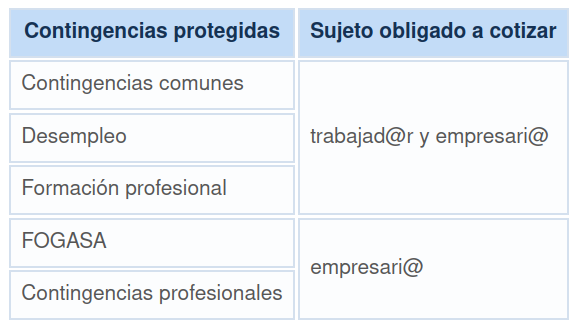
\includegraphics[scale=0.48]{obligacion-cotizacion.png}
    \caption{Obligación de cotización}
\end{figure}

El \textbf{sujeto responsable} del \textbf{pago de las cuotas} es el \textbf{empresario}, que deberá ingresar conjuntamente su cuota (\textbf{cuota patrona}l) y la de sus trabajadores (\textbf{cuota obrera}), que descontará cada mes a sus trabajadores en el momento de abonarles sus retribuciones. De no efectuarse este descuento en el momento señalado, no podrá realizarlo posteriormente, quedando obligado a ingresar la totalidad de las cuotas a su exclusivo cargo. Igualmente, la \textbf{retención indebida} por el empresario de las cuotas descontadas a sus trabajadores  le hará incurrir en responsabilidad frente a éstos y frente a la Seguridad Social, sin perjuicio de las responsabilidades penales o administrativas.

La \textbf{obligación de cotizar} nace en el momento en que \textbf{comienza la relación laboral}, incluido el período de prueba, y se mantiene mientras el trabajador/a permanezca dado de alta, extinguiéndose cuando sea cursada la baja, si esta se ha cesado la actividad laboral. En todo caso, esta obligación económica se \textbf{suspenderá} durante la \textbf{huelga} y el \textbf{cierre patronal}, siempre que la empresa presente los partes de baja en el plazo de 3 días, en otro caso, subsistirá la obligación de cotizar durante estos períodos.

Hay que tener en cuenta que la \textbf{obligación de cotizar permanece} en ciertos supuestos denominados ``\textbf{situaciones asimiladas de alta}'', pese a que se ha cesado la actividad laboral. Estos supuestos son los siguientes:

\begin{itemize}
    \item Los casos de \textbf{incapacidad temporal}, \textbf{riesgo durante el embarazo}, \textbf{maternidad} y \textbf{riesgo} durante la \textbf{lactancia natural}.
    \item Cuando el trabajador desempeñe \textbf{deberes} de \textbf{carácter público} o \textbf{cargos sindicales}, siempre que no den lugar a una excedencia.
    \item Situaciones de \textbf{desempleo total} con derecho a prestación.
    \item Otras ocasiones en las que se mantenga la obligación de cotizar (\textbf{permisos} y \textbf{licencias}).
\end{itemize}


\subsection{Determinación de la Cuota Patronal y Obrera}
Las \textbf{cuotas} son las cantidades a ingresar en la Tesorería General de la Seguridad Social. Se obtienen aplicando un porcentaje, llamado \textbf{tipo de cotización}, a una cantidad denominada \textbf{base de cotización} que se calcula según el salario mensual del trabajador.

\subsubsection{Tipos de Cotización}
Los \textbf{tipos de cotización }son los \textbf{porcentajes aplicables} a las bases de cotización para determinar las cuotas patronales y obreras que se deben ingresar en la Tesorería General de la Seguridad Social.

A partir del \textbf{1 de Enero de 2011}, los tipos de cotización en el Régimen General de la Seguridad Social son lo que se recogen en la siguiente tabla:

\begin{figure}[H]
    \centering
    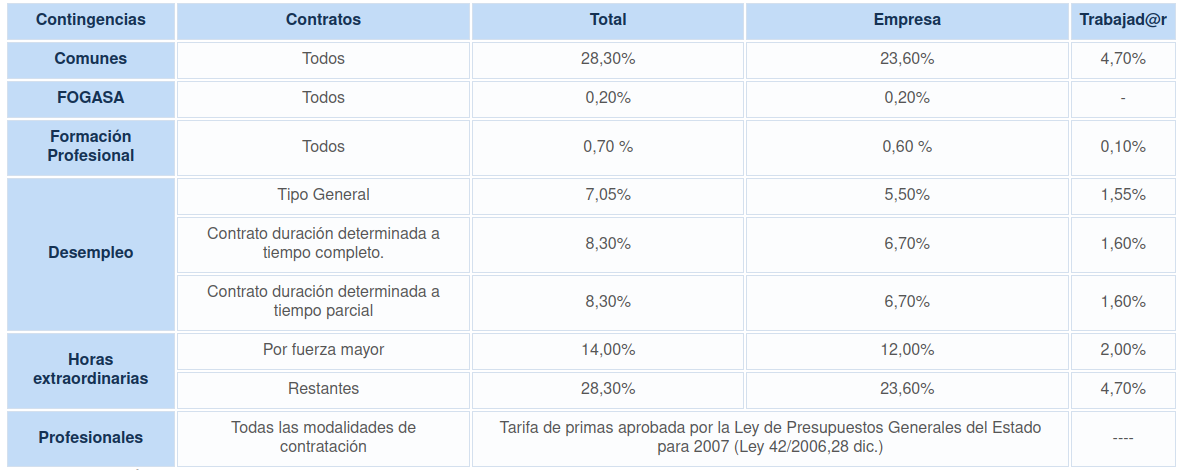
\includegraphics[scale=0.34]{tipos-cotizacion.png}
    \caption{Tipos de cotización en RG de la SS}
\end{figure}

\subsubsection{Base de Cotización}
La \textbf{base de cotización} (BC), está constituida por la renumeración total que tenga derecho a percibir el trabajador mensualmente por el trabajo realizado por cuenta ajena, con las excepciones señaladas por el \textbf{TRSS} (Art. 109.2) referidas a ciertas excepciones salariales.

La \textbf{normativa} sobre esta materia distingue entre los siguiente \textbf{tipos de cotización}:

\begin{itemize}
    \item \textbf{Base de Cotización por Contingencias Comunes}: para su determinación, se \textbf{computa el salario} correspondiente al mes a que se refiere la cotización, \textbf{excepto} las \textbf{horas extraordinarias}. A esta cantidad, se le añade la \textbf{parte proporcional} de las \textbf{pagas extraordinarias} y las \textbf{percepciones extrasalariales} cuando excedan los límites establecidos legalmente (RGCL), computándose tan solo el exceso. La base así calculada, deberá estar entre la \textbf{base mínima} y la \textbf{base máxima} del \textbf{grupo de cotización asignado} al trabajador en función de su categoría profesional, de no estarlo, se cotizará por la mínima o máxima según la que la resultante sea inferior o superior a aquella.

    \item \textbf{Base de Cotización por Contingencias Profesionales}: se computa aplicando las mismas reglas que para la BC por contingencias comunes, con la diferencia de que a este se le añaden las \textbf{horas extras}. La base obtenida deberá estar entre los topos mínimos y máximos absoluto, y en caso de sobrepasarlos, cotizará por estos.

    \item \textbf{Base de Cotización por Horas Extraordinarias}: se cotizará por las horas extras, siendo esta base de cotización igual al importe percibido por tales conceptos retributivos.
\end{itemize}

\section{Acción Protectora de la Seguridad Social}
Se entiende por \textbf{acción protectora} al conjunto de situaciones de necesidad protegidas por el Sistema de la Seguridad Social y los mecanismos de protección o prestaciones que se otorgan a los beneficiarios.

Nuestra Constitución de 1978 pretende alcanzar un Sistema de la Seguridad Social que proteja a toda la población en cualquier situación de necesidad, como así lo establece el Art. 41 de la Constitución Española.

Dentro de esta protección, podemos diferencias dos criterios de clasificación, que son:


\begin{itemize}
    \item \textbf{Ámbito}: podemos distinguir entre \textbf{prestaciones en servicios} y \textbf{prestaciones en dinero}.
    \item \textbf{Requisitos}: en este caso distinguiremos entre \textbf{protección contributivo} y \textbf{protección no contributiva}.
\end{itemize}

En los siguiente puntos vamos a estudiar estos conceptos y a estudiar en que consisten cada uno.

\subsection{Ámbito de la Acción Protectora}
Para reparar o superar las situaciones de necesidad derivadas de los riesgos o contingencias, ya sean debidas a la ausencia de ingresos (desempleo, incapacidad, vejez, ...) o al aumento de gasto (asistencia sanitaria, cargas familiares, ...), la seguridad social establece una serie de medidas técnicas o económicas, denominadas \textbf{prestaciones}, cuya finalidad es garantizar la recuperación de cada individuo y mantener la seguridad económica.

Actualmente, la protección del Sistema de la Seguridad Social no se extiende a cualquier riesgo, sino solo a los expresamente protegidos, siendo además esta protección diferente dependiendo del Régimen de la Seguridad Social del que se trate y de que la situación de necesidad se derive de contingencias o riesgos profesionales o comunes.

Con carácter general, la \textbf{acción protectora} actual del Sistema de la Seguridad Social comprende:
\begin{itemize}
    \item La \textbf{asistencia sanitaria} en los casos de maternidad, enfermedad y accidente, sean comunes o laborales.
    \item La \textbf{recuperación profesional}, como rehabilitación funcional, orientación y readaptación profesionales.
    \item \textbf{Prestaciones económicas} en la situaciones de incapacidad temporal, maternidad, paternidad, suspensión por riesgo durante el embarazo y lactancia natural, ademá s de prestaciones por desempleo.
    \item \textbf{Pensión} de jubilación, invalidez, muerte y supervivencia.
    \item \textbf{Prestaciones familiares} por hijos a cargo.
    \item  La \textbf{asistencia social} y \textbf{servicios sociales} de reeducación y rehabilitación de inválidos y de asistencia a la tercera edad, así como en otras aquellas materias en las que se considere conveniente.
    \item \textbf{Mejoras voluntarias} concedidas por las \textbf{empresas}, como seguros de vida, planes de pensiones, ayudas, etc...
\end{itemize}

Esta relación no es una lista cerrada, ya que la TGSS deja abierta la posibilidad de que se otorguen prestaciones económicas ante los riesgos y situaciones que se determinen legalmente en el futuro.

Como podemos ver en esta lista, podemos distinguir principalmente dos tipos de prestaciones, las \textbf{prestaciones económicas} y las \textbf{prestaciones de servicios o en especie}. En la siguiente tabla podemos ver un resumen de estos dos tipos:

\begin{figure}[H]
    \centering
    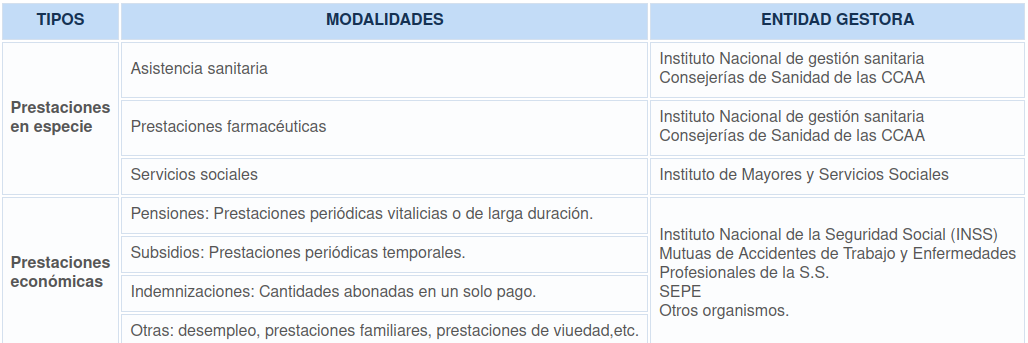
\includegraphics[scale=0.45]{prestaciones-ss.png}
    \caption{Tipos de prestaciones de la Seguridad Social}
\end{figure}

Como podemos ver en la tabla, hay diferentes modalidades de prestaciones, las cuales estarán gestionadas por un organismo u otro. A pesar de sus diferencias, todas estas prestaciones tienen unas \textbf{características} comunes que son las siguientes:
\begin{itemize}
    \item \textbf{Son embargables} en los mismos términos que el salario.
    \item El \textbf{derecho a reconocimiento} de las prestaciones \textbf{prescribe a los 5 años}, contados desde el día siguiente al hecho causante, salvo las de jubilación, muerte y supervivencia que son imprescriptibles.
    \item Por regla general, \textbf{las pensiones} de la Seguridad Social son \textbf{incompatibles entre sí}, salvo que se hubiera cotizado en dos o más Regímenes de la Seguridad Social. Un ejemplo de excepción al principio de incompatibilidad es la pensión de viudedad.
    \item Se \textbf{revalorizan cada año} según el incremento del Indice de Precios al Consumo (IPC).
\end{itemize}

\subsection{Requisitos de Acceso a la Acción Protectora}
El \textbf{derecho a las prestaciones} de la Seguridad Social se condiciona por la ley al cumplimiento de una serie de requisitos que varían según si estas prestaciones son contributivos o no contributivas.

\begin{enumerate}[label=(\Alph*)]
    \item \textbf{La protección contributiva}: en esta, el nivel de recursos económicos del beneficiario no es un factor a tener en cuenta, siendo los requisitos básicos de acceso a esta protección los siguientes:
    \begin{enumerate}
        \item Estar \textbf{afiliado a la Seguridad Social} y en situación de \textbf{alta} o \textbf{alta asimilada} en el momento de producirse el hecho causante, por lo que será preciso que el empresario haya cumplido previamente con estas obligaciones legales. No obstante, la ley admite que en determinados casos en los que el contrato de trabajo estaba suspendido (incapacidad temporal, maternidad, etc...) e incluso extinguido (desempleo), el trabajador siga bajo la protección del Sistema. Estas las llamadas \textbf{situaciones de alta asimilada}, aunque en estas no siempre se tiene derecho a todas las prestaciones que otorga el Sistema, fijando la ley en cada caso que prestaciones podrán ser concedidas.

        \item Tener cubiertos los \textbf{períodos de cotización previos}, también llamados \textbf{períodos de carencia}, que en cada caso sean exigibles, aunque algunos están exceptuados del cumplimiento de este requisito. Así ocurre con las prestaciones derivadas de accidentes, sean laborales o no, y de enfermedad profesional.
    \end{enumerate}

    La cuantía de las prestaciones contributivas es variables, pues se calculan aplicando unos porcentajes, que veremos al estudiar cada tipo de prestación, sobre las denominadas \textbf{bases reguladoras}, que se obtienen a partir de las bases de cotización de cada trabajador anteriores al hecho causante, de forma que cuanto mayores sean las bases de cotización, mayor será la cuantía de la prestación.

    \item \textbf{La protección no contributiva}: a diferencia de la anterior, esta condicionada a la insuficiencia de ingresos del beneficiario y a que tenga su residencia en territorio español. Por consiguiente, se concederán prestaciones económicas no contributiva de cuantía fija a personas no afiliadas, ni en alta, o que estando afiliadas y alta no hayan cotizado el periodo de carencia exigido para acceder a las prestaciones contributivas.

    Las únicas prestaciones no contributivas previstas en las actualidad son las siguientes:
    \begin{itemize}
        \item Los servicios de asistencia sanitaria y servicios sociales.
        \item Las pensiones no contributivas por invalidez y jubilación.
        \item Las asignaciones de la Seguridad Social por hijo a cargo.
        \item Pensiones por ancianidad a favor de emigrantes españoles.
        \item Prestación económica a favor de españoles emigrantes durante la Guerra Civil.
    \end{itemize}
\end{enumerate}

Cabe destacar que en relación a la \textbf{asistencia sanitaria}, \textbf{protección por desempleo} y \textbf{situaciones de necesidad} derivadas de riesgos o \textbf{contingencias profesionales}, siempre se considera que el trabajador se encuentra en situación de \textbf{alta de pleno derecho}, aunque el empresario hubiera incumplido sus obligaciones de afiliación, alta y cotización, aplicándose en estos casos el ``\textbf{principio de automaticidad de las prestaciones}'', lo cual implica que la Entidad Gestora de la Seguridad Social (INSS), concederá protección de forma automática al trabajador y posteriormente exigirá responsabilidades al empresario infractor por sus incumplimientos.

\section{Prestaciones Económicas Contributivas}
Como hemos comentado en el epígrafe anterior, las \textbf{prestaciones económicas contributivas} son aquellas en las que el trabajador tiene que estar dado de alta en la seguridad social y haber cotizado un tiempo determinado en el momento del hecho causante.

En los siguiente apartados estudiaremos las diferentes prestaciones contributivas de la Seguridad Social, por el ser el tipo más importante y el prototipo de sistema, dado el amplio colectivo asegurado en el mismo.

Dentro de las prestaciones que estudiaremos también incluiremos el desempleo, pero dada su trascendencia lo estudiaremos en un punto a parte, estudiando tanto su modalidad contributivo como no contributiva.

En la siguiente tabla puedes ver un resumen de las prestaciones que vamos a estudiar en los siguientes puntos:

\begin{figure}[H]
    \centering
    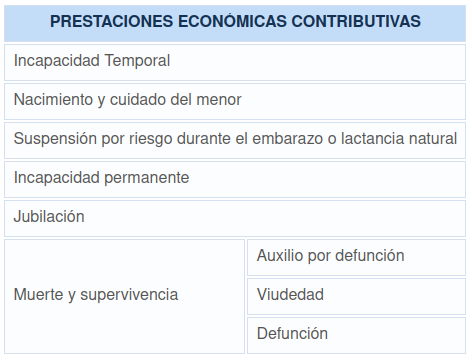
\includegraphics[scale=0.60]{prestaciones-contributivas.png}
    \caption{Prestaciones contributivas}
\end{figure}

\subsection{Incapacidad Temporal}
La \textbf{situación protegida}, dentro de la incapacidad laboral,es la \textbf{alteración temporal} de la \textbf{salud} del trabajador y exige asistencia sanitaria, derivada de enfermedad (común o profesional) o accidente (común o laboral) siempre que se prevea su curación.

Las \textbf{principales características} de esta protección son la siguientes:

\begin{itemize}
    \item \textbf{Duración}: tendrá una duración máxima de 12 meses, prorrogables por otros 6 cuando sea previsible su curación. Agotado el plazo, el INSS será el único competente para adoptar algunas de las siguientes medidas:
    \begin{enumerate}
        \item Conceder una \textbf{prorroga} de 6 meses.
        \item Iniciar un expediente de \textbf{incapacidad permanente} si no se prevé la curación.
        \item Emitir el \textbf{alta médica}.
    \end{enumerate}

    \item \textbf{Beneficiarios}: son los \textbf{trabajadores} integrados en el \textbf{Régimen General}, siempre y cuando estén afiliados y en situación de alta o alta asimilada en el momento de producirse el hecho causante, siendo necesario acreditar un \textbf{período previo de cotización} de \textbf{180 días} en los \textbf{5 años previos} al hecho causante. Si este fuera una \textbf{enfermedad común}, no se exige período de carencia.

    \item \textbf{Prestación Económica}: consiste en un subsidio temporal cuya cuantía dependerá del hecho causante, pudiendo ser este:

    \begin{itemize}
        \item \textbf{Por contingencias comunes}: esta es la causada por una enfermedad común o un accidente no laboral. En la siguiente tabla podemos ver la cuantía de la prestación económica:

        \begin{figure}[H]
            \centering
            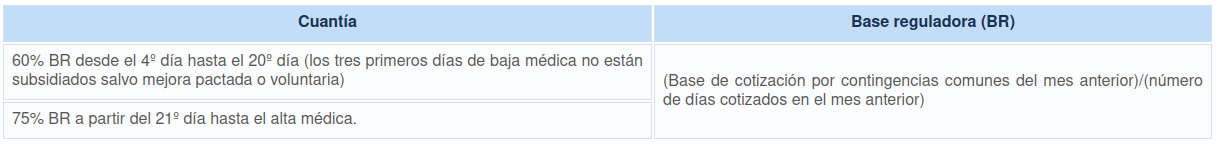
\includegraphics[scale=0.35]{it-comunes.png}
            \caption{Incapacidad Temporal por contingencias comunes}
        \end{figure}

        En este caso, la \textbf{entidad pagadora} dependerá del periodo en el que se encuentre la prestación, siendo:

        \begin{itemize}
            \item Desde el \textbf{4º al 15º día}, ambos inclusive, el subsidio lo abona el \textbf{empresario} a su cargo exclusivo.
            \item A partir del \textbf{día 16º}, será abonado por la \textbf{entidad aseguradora} (INSS, Mutua, etc..).
        \end{itemize}

        \item \textbf{Por contingencias profesionales}: en este caso, el hecho causante es una enfermedad o accidente laboral. Las cuantías por este tipo de contingencia las podemos ver en la siguiente tabla.

        \begin{figure}[H]
            \centering
            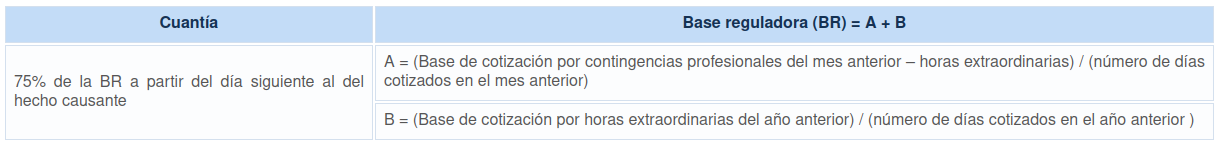
\includegraphics[scale=0.35]{it-profesionales.png}
            \caption{Incapacidad Temporal por contingencias profesionales}
        \end{figure}

        En este caso, la \textbf{entidad pagadora} será la \textbf{aseguradora}, que abonará la cantidad desde el mismo día del hecho causante.
    \end{itemize}
\end{itemize}

Hay que tener en cuenta que en aquellos períodos en los que el subsidio corre a cargo de la \textbf{entidad aseguradora}, el \textbf{pago se realizará} por la \textbf{empresa} por delegación, que posteriormente compensará las cantidades abonadas a los trabajadores que hayan causado baja médica con las cuotas que debe ingresar mensualmente a la TGSS.

\subsection{Nacimiento y Cuidado de Menor}
Las \textbf{situaciones protegidas} en esta prestación son las \textbf{suspensiones de contrato} debidas a \textbf{nacimiento}, \textbf{adopción} o \textbf{acogimiento}, siempre que su duración no sea inferior a \textbf{1 año}, de menores de seis años o menores de 18 años con discapacidad, o que por circunstancias y experiencias personales, o por provenir del extranjero, tengan especiales dificultades de inserción social y familiar debidamente acreditadas.

Esta prestación esta regulada por el \textbf{Cap. VI} del \textbf{Título II TGSS}, Ley 39/1999, para promover la conciliación familiar y laboral de las personas trabajadores desarrollado por el \textbf{RD 295/2006}, 6 de Marzo y \textbf{Real Decreto-Ley 6/2019}, 1 de Marzo.

Las \textbf{principales características} de esta prestación son:

\begin{itemize}
    \item \textbf{Duración}: desde el 1 de Enero de 2021 es de \textbf{16 semanas ampliables} en caso de parto, adopción o acogimiento múltiple, aumentando en \textbf{2 semanas más} por cada hijo a partir del segundo o cuando se trate de hijos discapacitados y por último por parto prematuro y hospitalización. El disfrute de tal período vendrá condicionado según sea por nacimiento, tanto de madre biológica como otro progenitor distinto a la madre biológica, o en caso de adopción, de guarda con fines de adopción y acogimiento.

    En caso de \textbf{fallecimiento del hijo} el período \textbf{no se verá reducido}, y en los casos de parto prematuro y aquellos en que, por cualquier causa, el \textbf{menor} deba \textbf{permanecer hospitalizado} a continuación del parto, una vez transcurridas las seis semanas posteriores al parto obligatorias para la madre, el \textbf{descanso podrá aplazarse} hasta el \textbf{alta hospitalaria} del menor.

    \item \textbf{Beneficiarios}: el derecho al descanso se recoge en \textbf{ambos progenitores} si trabajan, no obstante, respetando siempre las 6 semanas posteriores al parto que son obligatorias disfrutarlas juntos. En los casos de adopción y acogimiento, este reparto será decidido por ambos adoptantes de mutuo acuerdo. Estos períodos podrán disfrutarse a \textbf{jornada completa} o a \textbf{tiempo parcial}, precio acuerdo de los empresarios los trabajadores.

    Los beneficiarios por tanto serán los \textbf{trabajadores de ambos sexos} en situación de afiliación y alta o situación asimilada de alta en el RG, siempre que acrediten un \textbf{período de cotización} que varia en función de la \textbf{edad} que tengan en la fecha del parto, adopción o acogimiento:

    \begin{enumerate}
        \item Si las personas trabajadoras tienen \textbf{menos de 21 años} de edad, no se exigirá período de cotización mínima.
        \item Si las personas trabajadores tienen entre \textbf{21 y 26 años} de edad, el período exigido será de \textbf{90 días cotizados} dentro de los \textbf{7 años} anteriores al inicio del descanso. Se considerará cumplido el mencionado requisito si acredita un total de \textbf{180 días cotizados} a lo largo de su \textbf{vida laboral}.
        \item Si las personas trabajadores tiene \textbf{mas de 26 años} de edad, el período mínimo de cotización exigido serán de \textbf{180 días} dentro de los \textbf{7 años anteriores} al inicio del descanso. También se verá cumplido este requisito si el trabajador certifica \textbf{360 días cotizados} a lo largo de su \textbf{vida laboral}.
    \end{enumerate}

    \item \textbf{Prestaciones Económicas}: las diferentes prestaciones económicas que se podrán obtener con esta prestación son las siguientes:

    \begin{itemize}
        \item \textbf{Subsidio del 100\%}  de la base reguladora, que será equivalente a la establecida en la prestación de incapacidad temporal derivada de contingencias comunes, iniciándose el pago del mismo el día que da comienzo el descanso.
        \item En caso de \textbf{parto múltiple}, uno de los progenitores tendrá derecho  a un \textbf{subsidio especial} por \textbf{cada hijo} a partir del \textbf{segundo}, equivalente a \textbf{seis semanas} de una cantidad igual al subsidio que perciba por el primero.
        \item Los trabajadores que, en caso de parto, \textbf{reúnan todos lo requisitos} establecidos para acceder a la prestación por maternidad, \textbf{salvo el período de cotización} establecido, serán benficiarios de un subsidio especial de cuantía igual al \textbf{100\% del IPREM} vigente en cada momento.

        Esta prestación será de \textbf{42 días naturales} a contar desde la fecha del parto. Dicha duración se \textbf{incrementará en 14 días naturales} en los casos de nacimiento de hijo de una \textbf{familia numerosa} o que, con tal motivo, adquiera dicha condición, o en una \textbf{familia monoparental}, o en los \textbf{supuestos de parto múltiple} o hijos afectados con una \textbf{grado de discapacidad} igual o superior al \textbf{65\%}.
    \end{itemize}

    La \textbf{entidad pagadora} de esta prestación será la \textbf{INSS} o \textbf{MATEPSS}.
\end{itemize}

\subsection{Suspensión por Riesgo en el Embarazo o Lactancia Natural}
Las \textbf{situaciones protegidas} por esta prestación son los períodos en que quede suspendido el contrato por la existencia de riesgo durante el embarazo, o posteriormente durante la lactancia natural, cuando resulte técnica u objetivamente imposible un cambio de puesto de la trabajadora por otro compatible con su estado.

La \textbf{normativa reguladora} de esta prestación la encontramos en el \textbf{Art. 26 de la Ley 31/1995}, de Prevención de Riesgos Laborales, \textbf{Ley 39/1999}, para promover la conciliación de la vida familiar y laboral de las personas trabajadoras desarrollado por el \textbf{R.D. 295/2009}, 6 de Marzo.

Las \textbf{principales características} de esta prestación son las siguientes:

\begin{itemize}
    \item \textbf{Duración}: la duración será \textbf{la necesaria} para la \textbf{protección de su seguridad y salud}, mientras persista la imposibilidad de reincorporarse a su puesto anterior u otro puesto compatible con su estado. Durante este período percibirá una prestación económica hasta la reincorporación de la mujer  a un puesto compatible con su estado o, en caso de \textbf{maternidad}, hasta \textbf{el parto}.  En caso de \textbf{lactancia natural}, el derecho se \textbf{extingue} cuando el \textbf{hijo cumpla 9 meses}.

    \item \textbf{Beneficiarias}: las trabajadoras \textbf{afiliadas y en alta} o \textbf{alta asimilada} en el momento de producirse el hecho causante, no siendo necesario acreditar ningún periodo de cotización previo.

    \item \textbf{Prestación Económica}: consiste en un subsidio del \textbf{100\% de la base reguladora}, que será el equivalente al establecida para la incapacidad temporal por contingencias profesionales.

    En este caso, la \textbf{entidad pagadora} será directamente el INSS o MATEPSS.
\end{itemize}

\subsection{Incapacidad Permanente}
La \textbf{situación protegida} con esta prestación es aquella en que el trabajador sea considerado \textbf{incapacitado de forma permanente}, situación que se da cuando un trabajador, tras haberse sometido al tratamiento médico prescrito, presenta reducciones anatómicas o funcionales graves y previsiblemente definitivas, que disminuyen o anulan su capacidad laboral.

La \textbf{normativa reguladora} de esta prestación se encuentra en el \textbf{Cap. XI, Título II de la LGSS}, el \textbf{R.D. 1132/2002}, la \textbf{Ley 52/2003} y el \textbf{R.D. 1795/2003}, 26 de Diciembre.

Las \textbf{principales características} de esta prestación son la siguientes:

\begin{itemize}
    \item \textbf{Duración}: es una prestación que no tiene una duración máxima. Si se ha mantenido hasta el momento de la jubilación se seguirá recibiendo el mismo importe, solo cambiando el concepto de incapacidad permanente a jubilación.

    \item \textbf{Grados}: dentro de la incapacidad permanente podemos encontrar diferentes grados de incapacidad que, como veremos en el siguiente punto, condicionarán la cuantía a recibir. Estos grados son:

    \begin{itemize}
        \item \textbf{Incapacidad Permanente parcial para trabajador habitual}: es la que ocasiona al trabajador un \textbf{disminución} no inferior al \textbf{33\%} del rendimiento normal para su profesión habitual sin impedirle realizar las tareas fundamentales de la misma.
        \item \textbf{Incapacidad Permanente total para trabajador habitual}: es aquella que \textbf{inhabilita} para \textbf{la realización} de todas o las \textbf{tareas fundamentales de su profesión}, siempre que pueda dedicarse a otra distinta.
        \item \textbf{Incapacidad Permanente Absoluta}: es aquella que \textbf{inhabilita} al trabajador por completo \textbf{para cualquier profesión}.
        \item \textbf{Gran Invalidez}: es la situación en la que un \textbf{trabajador}, como consecuencia de pérdidas anatómicas y funcionales, \textbf{necesita de la asistencia} de otra persona para los \textbf{actos más esenciales de la vida}, tales como vestirse, desplazarse comer o análogos.
    \end{itemize}

    \item \textbf{Beneficiarios}: los trabajadores \textbf{afiliados} y en \textbf{alta} o \textbf{situación asimilada} que reúnan el período de carencia exigido legalmente cuando la incapacidad derive de enfermedad común. No se exige periodo de cotización previo si el hecho causante fue un accidente, común o laboral, o una enfermedad profesional.

    \item \textbf{Prestación Económica}: la prestación económica dependerá del grado de incapacidad que tenga reconocido el trabajador. En la siguiente tabla, podemos ver las diferentes prestaciones a las que se tiene derecho según el grado:

    \begin{figure}[H]
        \centering
        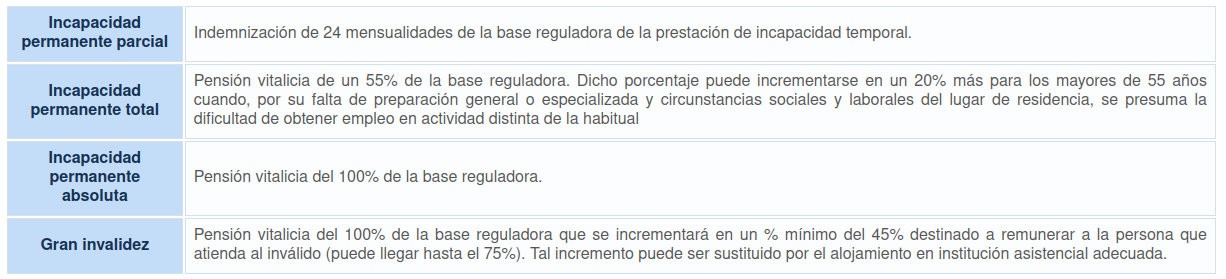
\includegraphics[scale=0.35]{prestaciones-incapacidad.png}
        \caption{Prestaciones económicas por incapacidad}
    \end{figure}

    La \textbf{Base Reguladora} (BR) se calculará de forma diferente dependiendo si la incapacidad es derivada de contingencias comunes o profesionales, así tenemos:

    \begin{enumerate}
        \item Cuando derive de \textbf{enfermedad común}: la base reguladora será igual a la \textbf{suma} de las 	\textbf{bases de cotización} de los últimos \textbf{96 meses} (8 años) inmediatamente anteriores al hecho causante, \textbf{dividido entre 112}.

        \item Cuando derive de ´\textbf{accidente no laboral}: la base reguladora será igual a la \textbf{suma} de las \textbf{bases de cotización} de un período ininterrumpido de \textbf{24 meses} elegido por el beneficiario  dentro de los \textbf{7 años} inmediatamente anteriores a la fecha del accidente.

        \item Cuando derive de \textbf{contingencias profesionales}: la base reguladora se calculará tomando las \textbf{retribuciones efectivas} percibidas en el momento del hecho causante de acuerdo con las reglas que fija el \textbf{Reglamento de Accidentes de Trabajo} de 1956.
    \end{enumerate}
\end{itemize}

Cabe mencionar que las \textbf{prestaciones económicas} por incapacidad permanente por riesgo profesional, en cualquiera de sus grados, \textbf{aumentarán} con un recargo variables entre el \textbf{30\% y el 50\%} cuando el \textbf{empresario} haya \textbf{incumplido} las medidas de seguridad e higiene en el trabajo, siendo el responsable el empresario incumplidor.

\subsection{La Jubilación}
Con esta prestación, la \textbf{situación protegida} es la vejez, pues a una edad avanzada el trabajador cesa su actividad laboral, y esto trae como consecuencia la carencia de ingresos. No obstante, se admite la \textbf{jubilación parcial} lo que permitirá al trabajador compatibilizar la pensión de jubilación con un trabajo a tiempo parcial en las condiciones legalmente previstas.

En estos momentos, tras la \textbf{reforma del sistema de pensiones} de 2011 y \textbf{su modificación}  del 2013, estamos en un \textbf{momento de transición} entre dos leyes que regulan el sistema de pensiones, de manera que la reforma del sistema de pensiones se va a ir \textbf{implantando poco a poco} desde el \textbf{año 2017 al 2027}. Por ello, habrá jubilados a los que les afectará la ley anterior y a otros que, gradualmente,les afectará la nueva ley hasta su implantación efectiva al 100\% en 2027.

Las \textbf{principales características} de esta prestación son las siguientes:

\begin{itemize}
    \item \textbf{Duración}: la duración de la jubilación será desde el momento en el que el trabajador haga efectiva su jubilación hasta la defunción de este.

    \item \textbf{Beneficiarios}: pasa ser beneficiario de la pensión de jubilación contributiva hay que cumplir una serie de condiciones, que dependiendo que que ley se aplique al trabajador en el momento de la jubilación serán los siguientes:
    \begin{itemize}
        \item Tener \textbf{cumplidos 65 años}, de los cuales al menos dos deberán estar comprendidos entre los 15 años inmediatamente anteriores al momento de causar el derecho, o bien acceder a la jubilación anticipada en el caso de los mayores de 61 años, conllevando una reducción del 6\% y el 8\% por cada año anticipado, en función de los años que se anticipe el cese del trabajo.
        \item Acreditar un \textbf{período de cotización} entre \textbf{15 y 35 años}.
    \end{itemize}


    \item \textbf{Prestación Económica}: la cantidad a percibir con esta prestación dependerá de los años cotizados, y de la base reguladora que hayamos tenido en estos, ya que según los años cotizados se aplicará un porcentaje a esta base reguladora. En la siguiente tabla, se puede observar la relación entre los años cotizados y el porcentaje a aplicar:

    \begin{figure}[H]
        \centering
        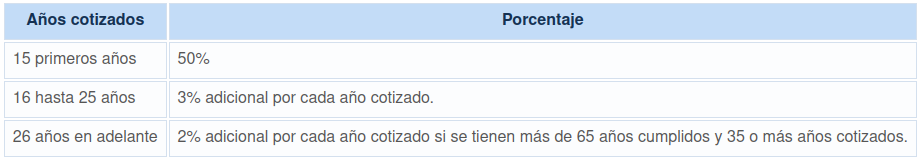
\includegraphics[scale=0.40]{prestacion-jubilacion.png}
        \caption{Años cotizados y porcentajes con la Ley Anterior}
    \end{figure}

    En este caso, la \textbf{base reguladora} se calcula sumando las bases de cotización de los \textbf{últimos 15 años} y \textbf{dividiendo entre 210}.
\end{itemize}

Con la \textbf{reforma de 2011 y 2013}, algunas de estas condiciones cambian, tanto en el punto de los beneficiarios como en el de la prestación económica. Estos cambios son los siguientes:

\begin{itemize}
    \item \textbf{Beneficiarios (Reforma de 2011/2013)}: tras la reforma se han aumentado la edad de jubilación así como los años máximos cotizados, quedando:

    \begin{itemize}
        \item Salvo excepciones, se deberán tener \textbf{67 años}.
        \item Haber cotizado entre \textbf{15 y 37 años} con carácter general, salvo excepciones.
    \end{itemize}

    \item \textbf{Prestación Económica (Reforma 2011/2013)}: en este caso, se han ampliado el número de años que se tiene que tener en cuenta para el cálculo de la base reguladora así como los porcentajes aplicados, quedando:

    \begin{itemize}
        \item Igualmente con \textbf{15 años} se percibe un \textbf{50\%}, pero después se suma por cada año un \textbf{2.28\%} anual hasta los \textbf{20 años y 8 meses} y un \textbf{2.16\%} anual hasta los \textbf{37 años}.
        \item Para calcular la base reguladora, se toma la media de lo \textbf{cotizado} en los \textbf{últimos 25 años}.
    \end{itemize}
\end{itemize}

Respecto a como se \textbf{esta aplicando} gradualmente la \textbf{reforma 2011/2013}, hay que tener en cuenta que \textbf{cada año }se van aplicando nuevas condiciones, aumentando los siguiente parámetros:

\begin{itemize}
    \item La \textbf{edad de jubilación} se \textbf{retrasa 1 o 2 meses} para ir pasando de los 65 años a los 67 años de la reforma.
    \item Los \textbf{años cotizados} para calcular la pensión aumentan cada año \textbf{1 año más}, para ir pasando de los últimos 15 años a los 25 años de la reforma laboral.
    \item Respecto a los \textbf{años cotizados} para obtener el \textbf{100\%} de la pensión, cada años se piden \textbf{1 y 2 meses más} de cotización para pasar de los 35 años de la anterior ley a los 37 años de la última reforma.
\end{itemize}

Para obtener más información sobre todos los requisitos así como de la aplicación gradual de la reforma de 2011/2013 podemos visitar la \href{https://www.seg-social.es/wps/portal/wss/internet/Trabajadores/PrestacionesPensionesTrabajadores/10963/28393/28396}{página de la Seguridad Social} acerca de las pensiones contributivas del Régimen General.

\subsection{Muerte y Supervivencia}
En esta prestación, el hecho causante es la \textbf{muerte o desaparición} del trabajador o pensionista, derivada de accidente o enfermedad, laboral o común, o en circunstancias que hagan presumible la muerte si transcurridos 90 días no hay noticias suyas.

Dos son la \textbf{situaciones de necesidad} de las que \textbf{protege esta prestaciones} y que se derivan de la muerte, por un lado, los \textbf{gastos del sepelio}, y por otro, la \textbf{supervivencia} de quienes \textbf{dependían materialmente del difunto}.

En la actualidad, esta prestación esta legislada en el \textbf{Cap. XIV LGSS}, \textbf{R.D 1465/2001} y \textbf{R.D 1795/2003}, 26 Diciembre, entre otras.

Las \textbf{principales características} de esta prestación son las siguientes:

\begin{itemize}
    \item \textbf{Causante de Derecho}: para que se pueda generar el derecho a esta prestación, el difunto o desaparecido, debe ser \textbf{pensionista} por incapacidad permanente o jubilación, o trabajador dado de \textbf{alta o situación asimilada} que acrediten un período mínimo de \textbf{cotización de 500 días} dentro de los \textbf{5 años} anteriores a su muerte, si el hecho causante fue una enfermedad común. De \textbf{no hallarse} en situación de \textbf{alta} o situación asimilada deberá acredita un \textbf{período de cotización} de \textbf{15 años}.

    \item \textbf{Beneficiarios}: esta prestación tiene se divide en dos modalidades, cada una de las cuales esta destinada a diferentes beneficiarios, siendo éstas las siguientes:

    \begin{itemize}
        \item \textbf{Pensión de Viudedad}: corresponde al \textbf{cónyuge superviviente}, no obstante cuando el fallecimiento derive de una enfermedad común anterior al enlace matrimonial, se requerirá además, que el \textbf{matrimonio} se hubiera celebrado con \textbf{1 año de antelación} como mínimo a la fecha del fallecimiento, salvo que existan hijos comunes o que hubieran convivido como pareja de hecho anteriormente, siempre que este período de convivencia sumado al del matrimonio supere los dos años. Tendrán así mismo derecho a pensión de viudedad los que conviviesen con el trabajador fallecido como \textbf{pareja de hecho} y acrediten que sus \textbf{ingresos} durante el año anterior natural no alcanzan los limites legales establecidos para estos supuestos.

        Para la Seguridad Social, se considera \textbf{pareja de hecho} la relación de afectividad entre dos personas que no tienen vínculo matrimonial con otras y acreditan, mediante certificado de empadronamiento, una \textbf{convivencia estable} y notoria anterior al fallecimiento y con una duración ininterrumpida \textbf{mínima de 5 años}.

        En los casos de \textbf{separación o divorcio}, el derecho de al pensión de viudedad corresponde a quien sea o haya sido cónyuge legítimo. Si hubiera otros beneficiarios con derecho a pensión de viudedad, esta será reconocida en \textbf{cuantía proporcional} al \textbf{tiempo vivido} por cada uno de ellos con el fallecido.

        La pensión de viudedad \textbf{se extinguirá} en los siguientes supuestos:

        \begin{itemize}
            \item Por contraer nuevo matrimonio o constituir pareja de hecho, salvo en las excepciones establecidas en al ley.
            \item Por declaración en sentencia firme de culpabilidad en la muerte del causante.
            \item Por comprobarse que no falleció el trabajado desaparecido en accidente.
            \item Cuando el pensionista separado o divorciado del fallecido conviviera maritalmente con otra persona.
        \end{itemize}

        \item \textbf{Prestaciones de Orfandad}: los beneficiarios de esta modalidad de la prestación son los siguientes:
        \begin{itemize}
            \item Los \textbf{hijos huérfanos}, incluidos los \textbf{adoptivos} si la adopción tuvo lugar como \textbf{mínimo 2 años} antes del fallecimiento del adoptante.
            \item Los \textbf{hijos} aportados al matrimonio por el \textbf{otro cónyuge}, siempre que este se hubiera celebrado 2 años antes, como mínimo, se pruebe además la convivencia habitual y la dependencia económica del fallecido, y no tenga derecho a otra pensión ni existan familiares con obligación y posibilidades de prestarle alimentos.
        \end{itemize}

        Los \textbf{hijos} deben ser \textbf{menores de 21 año} o \textbf{mayores discapacitados}, aunque este límite se amplía a \textbf{25 años} inclusive en caso de \textbf{orfandad absoluta}, siempre que no realice trabajo alguno, o cuando realizándolo, los ingresos anuales que se obtengan resulten inferiores a la cuantía del SMI anual vigente.
    \end{itemize}

    \item \textbf{Prestación Económica}: la cuantía de la \textbf{base reguladora} variará según el hecho causante de la muerte, quedando esta así:

    \begin{itemize}
        \item Si el fallecido estaba en \textbf{situación de alta} y la muerte se debió a una \textbf{contingencia común}, la base reguladora será el cociente que resulte de \textbf{dividir entre 28} las \textbf{sumas} de las \textbf{bases de cotización} en un período ininterrumpido de \textbf{24 meses} elegido por los beneficiarios dentro de los \textbf{15 años anteriores} a la fecha de su muerte.
        \item Si el fallecimiento se debió a un \textbf{riesgo profesional}, la base reguladora se calcula sobre los \textbf{salaos reales} de acuerdo a las \textbf{reglas} establecidas en el \textbf{Reglamento de Accidentes de Trabajo} de 1956.
        \item En caso de fallecimiento por \textbf{acto terrorista}, la base reguladora se determina \textbf{dividiendo por 14} el resultado de \textbf{multiplicar por 12} la última base de cotización.
        \item Si en fallecido era un \textbf{pensionista} por jubilación o invalidez, la base reguladora será la misma que sirvió para determinar su pensión con las revalorizaciones que correspondan.
    \end{itemize}

    Cuando la muerte fue causada por \textbf{actos de terrorismo}, se abonan al cónyuge viudo y a los huérfanos \textbf{pensiones extraordinarias}, cuyo importe es el \textbf{200\%} de la pensión que les correspondiera. Además, algunos \textbf{convenios colectivos} establecen mejoras de estas prestaciones en caso de muerte derivada por accidente laboral.
\end{itemize}

\section{El Desempleo}
La \textbf{protección por desempleo} es gestionada por el Servicio Público de Empleo Estatal (SEPE) y se estructura en un nivel contributivo y un nivel asistencial, que examinaremos por separado dada la diferente finalidad y régimen jurídico de cada uno de ellos.

Esta prestación \textbf{protege} a los trabajadores en \textbf{situación legal de desempleo}, considerándose está aquella en la que están quienes pudiendo y queriendo trabajar, pierden su empleo o ven reducida su jornada ordinaria de trabajo al menos en una tercera parte.

Independientemente de la modalidad, todos los beneficiarios deben cumplir los siguientes requisitos:

\begin{enumerate}
    \item Hallarse en \textbf{situación} legal de \textbf{desempleo}.
    \item \textbf{Estar afiliados} y no haber cumplido la edad ordinaria de jubilación.
    \item Esta \textbf{inscrito} como \textbf{demandante de empleo} en las oficinas del SEPE.
    \item Suscribir un \textbf{compromiso de actividad}, entendiéndose a estos efectos, el compromiso que adquiere el trabajador desempleado de buscar activamente empleo, aceptar una colocación adecuada y participar en las acciones de motivación, información, orientación, reconversión o inserción profesional que determine el SEPE, así como cumplir las restantes obligaciones previstas en al ley.
\end{enumerate}

Actualmente esta prestación esta regulada en el \textbf{Titulo III del TRSS}, \textbf{R.D 625/1985}, \textbf{Ley 45/2002}, \textbf{R.D 1975/2008}, \textbf{RDL 2/2009}, entre otras leyes.

Para que exista una \textbf{situación legal de desempleo} protegible es preciso que la \textbf{perdida de empleo} se haya producido por alguna de las siguientes \textbf{causas}:

\begin{itemize}
    \item Suspensión de la relación labora en virtud de un \textbf{Expediente de Regulación de Empleo} (ERE) o por tratarse de una \textbf{victima de violencia de género} (desempleo temporal).
    \item \textbf{Reducción de jornada} o \textbf{salario} de al menos una tercera parte (desempleo parcial).
    \item Extinción de la relación laboral por alguna de las siguientes causas (desempleo total):
    \begin{itemize}
        \item Por \textbf{ERE}, \textbf{causas objetivas}, o por la \textbf{muerte}, \textbf{jubilación} o \textbf{incapacidad} del \textbf{empresario}.
        \item \textbf{Despido disciplinario}, procedente o improcedente, sin necesidad de reclamación judicial.
        \item \textbf{Resolución} del contrato a \textbf{instancia del trabajador} en los supuestos de \textbf{traslado}, \textbf{modificación} sustancial de las \textbf{condiciones} de trabajo, \textbf{incumplimiento grave} por parte del empresario de sus obligaciones o cuando se trate de una \textbf{victima de violencia de género}.
        \item \textbf{Extinción del contrato temporal} por expiración del tiempo convenido o realización de la obra o servicio contratado, siempre que el trabajador no se haya negado a prorrogar su duración.
        \item Extinción durante un \textbf{período de prueba} a \textbf{instancia del empresario}, siempre que la extinción de la relación laboral anterior a su contratación se hubiera producido por causas ajenas a su voluntad, o haya transcurrido un plazo de tres meses desde dicha extinción.
        \item Extinción del contrato por \textbf{invalidez permanente} total del \textbf{trabajador}.
    \end{itemize}
\end{itemize}

\textbf{No se encuentra} en \textbf{situación legal de desempleo} aquellos trabajadores que cesen voluntariamente en el trabajo, y quienes aún encontrándose en alguna de las situaciones previstas en el apartado anterior, no acrediten su disponibilidad para buscar activamente empleo y para aceptar colocación adecuada a través del compromiso de actividad.

Los \textbf{sujetos protegidos} por la prestación de desempleo son, entre otros:
\begin{enumerate}
    \item Los \textbf{trabajadores por cuenta ajena} incluidos en el Régimen General y los Regímenes Específicos que protegen frente a este riesgo o contingencia.
    \item Los \textbf{liberados de prisión}.
    \item Los \textbf{emigrantes retornados} cuando el retorno se produce por haberse extinguido una relación laboral en el extranjero y no tienen derecho a prestación por desempleo en el país de origen.
\end{enumerate}

\subsection{Protección por Desempleo Contributivo}
Los \textbf{beneficiarios del nivel contributivo} de la protección por desempleo, además de los requisitos mencionados en el punto anterior, deben cumplir:

\begin{itemize}
    \item \textbf{Estar afiliados}  y en \textbf{situación de alta} o asimilada.
    \item Acreditar un \textbf{período mínimo} de cotización de \textbf{360 días} dentro de los \textbf{6 años anteriores} a la situación legal de desempleo, computándose únicamente las cotizaciones que no hayan sido tenidas en cuenta para el reconocimiento de un derecho anterior, a excepción de las prestaciones abonadas a las victimas de violencia de género que no serán tenidas en cuenta a tales efectos.
\end{itemize}

Las \textbf{personas que cumplan los requisitos} legalmente previstos, deberán \textbf{solicitar} en el \textbf{SEPE} el reconocimiento del derecho a la prestación por desempleo, que nacerá a partir de la fecha en que se inició la situación legal de desempleo, siempre que lo \textbf{solicite} en los \textbf{15 días hábiles} siguientes, pues quienes presenten la solicitud \textbf{fuera de plazo}, tendrán derecho a la prestación pero esta nacerá a partir de la fecha de la solicitud, por lo que \textbf{perderán tantos días} como medien entre la fecha que hubiera tenido lugar el nacimiento del derecho y aquella en la que efectivamente se haya formulado la solicitud, ademas de descontarse otros tantos días por el retraso desde el primer día que podía haberlo solicitado hasta que lo pidió realmente.

En caso de que el \textbf{período de vacaciones anual} no se haya disfrutado antes de finalizar la relación laboral, la situación de desempleo y el nacimiento del derecho a las prestaciones tendrá lugar una vez transcurrido dicho periodo que habrá sido abonado por la empresa en el finiquito.

La \textbf{duración y la cuantía} de la prestación económica por desempleo, total o parcial, estará en función de los \textbf{períodos cotizados} en los \textbf{últimos 6 años} anteriores a la situación legal de desempleo y a las \textbf{bases de cotización} de los \textbf{últimos 180 días}, sin que se puedan sobrepasar los límites máximos y mínimos legalmente previstos que se calculan con el Indicador Público de Rentas de Efecto Múltiple (IPREM), que en 2023 está situado en 600€/mes.

En los caso de desempleo parcial, la \textbf{cuantía de la prestación} se reduce en proporción a la jornada de trabajo que desarrolle el trabajador, pero esto no influye en la duración de la prestación.

Así, la \textbf{duración} de la prestación de desempleo será la que vemos en la siguiente tabla:

\begin{figure}[H]
    \centering
    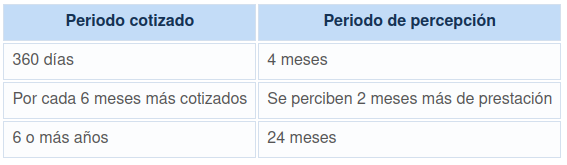
\includegraphics[scale=0.60]{duracion-desempleo.png}
    \caption{Duración prestación de desempleo}
\end{figure}

Por otro lado, la \textbf{cuantía} de la prestación por desempleo será un porcentaje aplicado al IPREM, como podemos ver en la siguiente tabla:

\begin{figure}[H]
    \centering
    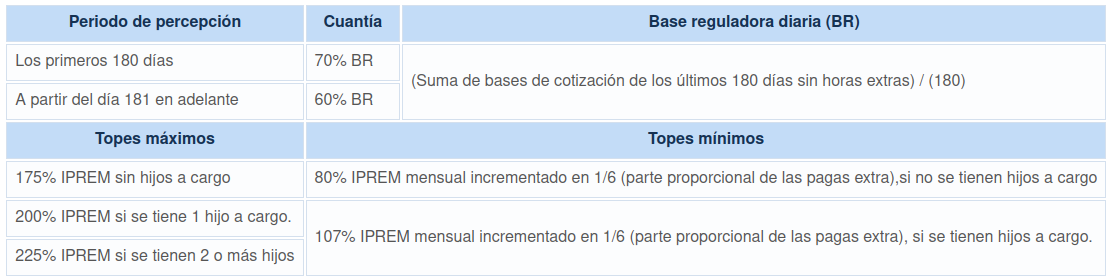
\includegraphics[scale=0.40]{cuantia-desempleo.png}
    \caption{Cuantía prestación de desempleo}
\end{figure}

Si la prestación se \textbf{inicio en 2023}, la cuantía de la misma, así calculada, en ningún caso podrá ser \textbf{inferior o superior} a los siguientes importes:

\begin{figure}[H]
    \centering
    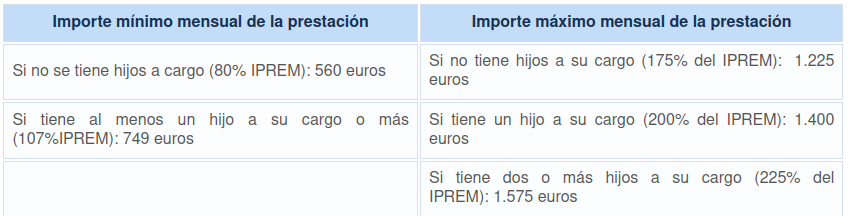
\includegraphics[scale=0.45]{minmax-desempleo.png}
    \caption{Cuantías mínimas y máximas desempleo}
\end{figure}

\textbf{Durante la percepción} de la prestación de desempleo el trabajador permanecerá en \textbf{alta} en la Seguridad Social y se efectuará la cotización por contingencias comunes. El abono de la aportación empresarial lo efectuará el SEPE en su totalidad y la aportación al trabajador será íntegra a cargo de este.

\subsubsection{Modalidades de Pago de la Prestación por Desempleo}
A la hora de recibir la prestación económica por desempleo, la ley contempla distintas modalidades de pago, que son las siguientes:

\begin{enumerate}
    \item \textbf{Pago Periódico}: esta es la forma más habitual y consiste en el pago de la prestación por desempleo por mensualidades vencidas durante el período reconocido.
    \item \textbf{Pago Único}: es pago único es una medida de fomento del empleo que pretende \textbf{facilitar la puesta en marcha} de \textbf{iniciativas de autoempleo} que consistan en iniciar una activad laboral como trabajador por cuenta propia o en incorporarse como socio trabajador o de trabajo en cooperativas o sociedades laborales o mercantiles en funcionamiento o de nueva creación. Las alternativas para recibir este pago dependerá de la iniciativa que vaya a llevar a cabo el trabajador, así:

    \begin{itemize}
        \item Como \textbf{trabajador autónomo}:
        \begin{itemize}
            \item Puede obtener en un \textbf{solo pago} la cantidad que \textbf{justifique como inversión} necesaria para iniciar la actividad, con el límite máximo del 60\% del importe total pendiente de percibir, elevándose al 100\% para hombres menores de 30 años y mujeres menores de 35 años en la fecha de la solicitud.

            Los trabajadores que acrediten estar afectados por un grado igual o superior al \textbf{33\% de discapacidad} podrán percibir el valor actual del importe de la prestación contributiva. Si no obtiene el total de la cuantía de su prestación en un solo pago, puede solicitar simultáneamente el abono del importe restante para financiar el coste de las cuotas mensuales de la Seguridad Social durante el desarrollo de su actividad.
            \item Puede solicitar y obtener exclusivamente la \textbf{cantidad que justifique} como \textbf{inversión}.
            \item Puede solicitar y obtener exclusivamente el \textbf{importe total} de la prestación pendiente a percibir para la \textbf{subvención} de las \textbf{cuotas mensuales} de las Seguridad Social.
        \end{itemize}

        \item Como \textbf{socio trabajador}:

        Cuando pretenda incorporarse de forma estable y a tiempo completo, como \textbf{socios trabajadores} en Cooperativas o en sociedades laborales, podrán capitalizar la prestación por el \textbf{importe igual} al de la \textbf{aportación a la cooperativa} o al \textbf{valor de las acciones} o \textbf{participaciones sociales} suscritas.

        Para poder llevar a cabo esta capitalización, el trabajador debe cumplir los siguiente requisitos:

        \begin{enumerate}
            \item Tener al menos \textbf{3 meses} de prestación por desempleo a percibir.
            \item \textbf{No haber} obtenido el reconocimiento de un \textbf{pago único} en los \textbf{últimos 4 años}.
            \item Que la \textbf{actividad} que va a desarrollar sea algunas de las siguiente:
            \begin{itemize}
                \item Actividad como trabajador autónomo.
                \item Constitución o incorporación a una sociedad cooperativa o laboral.
            \end{itemize}
            \item \textbf{Iniciar la actividad} en un plazo máximo de \textbf{un mes} desde la resolución de la concesión del derecho y en todo caso, con fecha posterior a la solicitud.
        \end{enumerate}
    \end{itemize}
\end{enumerate}

La prestación por desempleo \textbf{se puede compatibilizar} con la \textbf{actividad profesional} y algunas otras prestaciones, pero solo en alguno de los siguientes casos:

\begin{itemize}
    \item Con el \textbf{trabajo retribuido} por \textbf{cuenta ajena} a \textbf{tiempo parcial}, incluido con un contrato por tiempo indefinido de apoyo a los emprendedores a tiempo parcial, sin perjuicio del descuento correspondiente a la cuantía de la prestación.
    \item Con el \textbf{trabajo por cuenta propia o ajena} a \textbf{tiempo completo} cuando este establecida la compatibilidad con algún \textbf{programa de fomento de empleo}.
    \item Con la \textbf{indemnización} que proceda de la extinción del contrato de trabajo.
    \item Con la \textbf{pensión de jubilación parcial} y con las pensiones o prestaciones de carácter económico de la Seguridad Social que hubieran sido compatibles con el trabajo que originó la prestación.
    \item Con las \textbf{becas y ayudas} que se obtengan por asistencia a acciones de \textbf{formación ocupacional} i para realizar \textbf{prácticas} en entidades públicas o privadas que formen parte de un plan de estudios y se produzca en el marco de colaboración entre dichas entidades y el centro docente que se trate.
    \item Con la realización de \textbf{trabajo de colaboración social}.
    \item Con las \textbf{prestación por hijo a cargo} de la Seguridad Social.
    \item Con el \textbf{ejercicio por designación} o \textbf{elección} de cargos públicos o sindicales retribuidos que supongan una dedicación parcial, sin perjuicio de la deducción correspondiente a la cuantía de la prestación.
\end{itemize}

\subsubsection{Suspensión y Extinción de la Prestación de Desempleo}
La suspensión o extinción de la prestación por desempleo consiste en la interrupción de la prestación, ya sea de forma temporal o indefinida por diferentes causas. En los siguientes puntos vamos a ver estas dos situaciones con más detalle.

La \textbf{suspensión del derecho} supone la interrupción del abono de las prestaciones por desempleo económicas y de la cotización a la Seguridad Social durante un período de tiempo estimado. Las \textbf{causas} que motivan esta suspensión pueden ser alguna de las siguientes:

\begin{enumerate}
    \item \textbf{Traslado de residencia al extranjero}, por un período medio continuado \textbf{inferior a 12 meses}, para la búsqueda o realización de un trabajo, perfeccionamiento profesional o cooperación internacional.
    \item La situación de \textbf{maternidad} o \textbf{paternidad}.
    \item Cumplimiento de condena de \textbf{privación de libertad}, salvo para trabajadores con cargas familiares y que no disponga de renta familiar alguna, en cuyo caso, continuará percibiendo la prestación.
    \item Realización de \textbf{trabajo por cuenta ajena} con una duración \textbf{inferior a 12 meses}.
    \item Realización de \textbf{trabajo por cuenta propia} con una duración \textbf{inferior a 24 meses}.
    \item \textbf{Sanción de suspensión} por una infracción leve o grave.
\end{enumerate}

En todos los \textbf{casos de suspensión}, salvo en el caso de sanción, el \textbf{trabajador debe solicitar} la reanudación del derecho a la Oficina del SEPE que le corresponda en un plazo de \textbf{15 días} desde la finalización de la causa de la suspensión y acreditar que continúa en situación legal de desempleo.

La \textbf{reanudación} supondrá el derecho de percibir la prestación de desempleo con la base reguladora y el porcentaje que correspondiese en el momento de la suspensión y por el período que restase, salvo en los casos de suspensión por sanción en los que se reducirá su duración por el tiempo que dure la sanción.

La \textbf{extinción de la prestación} supone la perdida del derecho a recibir la prestación de desempleo de forma definitiva, por lo menos hasta que se genere de nuevo el derecho tras el periodo de cotización necesario.

Las \textbf{causas} por las que se puede extinguir la prestación de desempleo son las siguientes:

\begin{enumerate}
    \item \textbf{Agotar el plazo de duración} reconocido para la prestación de desempleo.
    \item \textbf{Rechazar una oferta de empleo} adecuada o \textbf{negarse a participar} en trabajos de colaboración social, programas de desempleo o acciones de promoción y formación profesional, salvo que existe causa justificada.
    \item \textbf{Ser sancionado} por alguna de las infracciones graves o muy graves tipificadas legalmente.
    \item \textbf{Cumplir la edad de jubilación}, salvo que el trabajador no tuviera periodo de cotización exigido para ello.
    \item Pasar a ser \textbf{pensionista de invalidez permanente} total, absoluta o gran invalidez, aunque en estos casos podrá optar entre seguir percibiendo la prestación hasta que se agote y luego pasar a cobrar la pensión que le corresponda, o bien percibir directamente la pensión de invalidez.
    \item Realizar una \textbf{trabajo por cuenta ajena} de duración superior o igual a \textbf{12 meses}, salvo que se trate de un trabajo a tiempo parcial, o un \textbf{trabajo por cuenta propia} de duración igual o superior a \textbf{24 meses}.
\end{enumerate}

\subsection{Protección por Desempleo Asistencia}
La \textbf{protección} en el \textbf{nivel asistencial} está prevista exclusivamente para los desempleados que no tenga derecho a la prestación de nivel contributivo, bien por no reunir los requisitos necesarios o por haber agotado la prestación contributiva.

Existen \textbf{diferentes tipos de subsidio} y en cada uno de ellos se exigen unos requisitos específicos, pero en todos los casos la ley exige unos \textbf{requisitos comunes} a todos estos que son los siguientes:

\begin{enumerate}
    \item La \textbf{insuficiencia de recursos o rentas} de cualquier naturaleza superiores al cómputo anual del \textbf{75\% del SMI}, sin computar la parte proporcional de las dos pagas extras.
    \item Encontrarse \textbf{inscrito como demandante de empleo} sin haber rechazado oferta de empleo adecuada ni haberse negado a participar, sin causa justificada, en acciones de promoción, formación o reconversión profesionales.
\end{enumerate}

Respecto a la \textbf{cuantía}, la ley fija una cuantía fija común a la mayoría de los diferentes subsidios de desempleo, la cual corresponde a un \textbf{80\% del IPREM}, que para el año \textbf{2023} es de \textbf{480€}.

Su \textbf{duración} será variable y dependerá del tipo de subsidio, siendo de \textbf{6 meses} prorrogables \textbf{hasta 18 meses} en algunos casos, y en otros dependerá de varios factores como la edad del trabajador, si tiene cargas familiares, días cotizados, etc.. Si el subsidio es para mayores de 52 años, se puede prolongar hasta la edad de jubilación.

Respecto a las \textbf{responsabilidades familiares}, se entiende que el trabajador tiene estás si se cumple:

\begin{enumerate}
    \item El cónyuge o los hijos menores de 25 años están a su cargo y no perciben ingresos superiores al 75\% del SMI vigente (750€).
    \item La suma de los ingresos de la unidad familiar, dividida entre el número de miembros de ésta no supera el 75\% del SMI vigente (750€)
\end{enumerate}

En la página del SEPE, podemos consultar \href{https://www.seg-social.es/wps/portal/wss/internet/InformacionUtil/44539/47006}{este triptico} con información más detallada sobre el subsidio por desempleo.

\chapter{Evaluación de Riesgos Profesionales}

En este tema vamos a estudiar los \textbf{riesgos profesionales} o \textbf{riesgos laborales}, entendiendo estos como todos los accidentes y enfermedades a los que esta expuesto un trabajador, ya sea en la empresa pública o privada, y que resultan como consecuencia de las labores que desempeña en su empleo.

También estudiaremos como realizar una correcta \textbf{evaluación} de estos riesgos, estudiando sus diferentes tipos y las consecuencias que pueden tener en el trabajador.

\section{El Trabajo y la Salud}
La \textbf{Organización Mundial de la Salud} (en adelante OMS) define la salud como el bienestar físico, psíquico y social completo, y no meramente la ausencia de enfermedad. El desequilibrio o la perdida de cualquiera de estos factores, implica el quebranto de la salud.

El \textbf{trabajo} determina en gran parte la salud de la personas. Gracias al trabajo una persona puede cubrir sus necesidades vitales, pero tanto la salud como la calidad de vida laboral, dependerán de las condiciones en las que éste se desarrolle.

En este aspecto, la \textbf{Constitución Española} (Art. 40.2), \textbf{obliga} a los \textbf{poderes públicos} a desarrollar y fomentar una \textbf{política de protección en el trabajo}. El derecho a la seguridad laboral también se especifica en el \textbf{Estatuto de los Trabajadores} en su articulo 19.1.

No obstante, la \textbf{principal norma} que regula en España todo lo relacionado con la seguridad  en las condiciones de trabajo se denomina \textbf{Ley de Prevención de Riesgos Laborales}, del 8 de Noviembre de 1985 (en adelante \textbf{LPRL}).

\section{Los Riesgos Profesionales: Concepto y Clasificación}
La \textbf{LPRL}, en el \textbf{artículo 4.2}, define el \textbf{riesgo laboral} como la posibilidad que tiene un trabajador de sufrir un determinado daño derivado de su trabajo. Los principales riesgos son físicos, químicos, biológicos, psicosociales y por sobrecarga física.

No todos los trabajadores y trabajadoras desarrollan su labor en las mismas condiciones, los mineros trabajan en la mina, los mecánicos en los talleres, las enfermeras en los hospitales, etc... Esto significa que en \textbf{cada trabajo} se dan condiciones laborales diversas, por lo que los \textbf{riesgos laborales} también son \textbf{diversos}.

La \textbf{LPRL} en el articulo 4.7 define las \textbf{condiciones de trabajo} como cualquier característica que pueda tener una influencia en la generación de riesgos para la seguridad y la salud del trabajador. Quedan específicamente incluidos en esta definición:

\begin{itemize}
    \item Las \textbf{características generales} de los \textbf{locales}, \textbf{instalaciones}, \textbf{equipos}, \textbf{productos} y \textbf{demás útiles} existentes en el lugar de trabajo.
    \item La \textbf{naturaleza y concentración} de los \textbf{agentes químicos}, \textbf{físicos} y \textbf{biológicos} que se encuentren presentes en el ambiente de trabajo. Por ejemplo: iluminación, condiciones térmicas, ruido, vibraciones, etc...
    \item Los \textbf{métodos de utilización} de los agentes mencionados en el punto anterior que influyan en la generación de riesgos.
    \item Todas aquellas \textbf{características del trabajo} que relativas a su organización y ordenación, influyen en la generación de riesgos. Por ejemplo: horarios, repetitividad, autonomía, retribución, turnos, etc...
\end{itemize}

Por lo tanto, existe gran relación entre el tipo de trabajo que se desarrolla y los riesgos a los que esta expuesto el trabajador, habiendo trabajos en los que hay más elementos o condicionantes que producir un riesgo laboral. Estos elementos o condicionantes  se denominan \textbf{factores de riesgo}.

Pero no todos los riesgos son \textbf{igual de peligrosos}, por eso hay que saber valorarlos en su justa medida. La LPRL en su artículo 4.2 indica \textbf{dos valores} que hay que tener en cuenta a la hora de \textbf{valorar} un riesgo:

\begin{itemize}
    \item La \textbf{probabilidad} de que se \textbf{produzca}.
    \item La \textbf{severidad} de las consecuencias.
\end{itemize}

Así, el \textbf{riesgo} más peligroso que existe se califica como \textbf{grave e inminente}, siendo aquel que resulta racionalmente probable que se materialice en un futuro inmediato provocando un daño grave en la salud de los trabajadores y trabajadoras.

\section{Factores de Riesgo}
Los \textbf{factores de riesgo} son los \textbf{elementos} o \textbf{conjunto variables} que están presentes en en las condiciones de trabajo y que pueden originar una disminución de la salud del trabajador.

Podemos \textbf{clasificar} los factores de riesgo en \textbf{tres grupos} principales:

\begin{itemize}
    \item \textbf{Riesgos Derivados de las Condiciones de Seguridad}: en este grupo se incluyen aquellas condiciones materiales que pueden dar lugar a accidentes de trabajo, incluyendo:
    \begin{itemize}
        \item Los lugares de trabajo.
        \item Máquinas y equipo de trabajo.
        \item Riesgos eléctrico y de incendio.
    \end{itemize}

    \item \textbf{Riesgos Derivados de las Condiciones Ambientales}: son factores del medio ambiente natural presentes en el ambiente de trabajo y que aparecerán de la misma forma o modificados por el proceso de producción y repercuten negativamente en la salud del trabajador. Se dividen en:
    \begin{itemize}
        \item \textbf{Contaminantes de Origen Físico}: entran dentro de esta categoría el ruido, vibraciones, temperatura, iluminación y las radiaciones.
        \item \textbf{Contaminantes de Origen Químico}: son sustancias químicas que durante la fabricación, transporte, almacenamiento o uso pueden incorporarse al ambiente en forma de aerosoles, gas o vapor, y afectar a la salud de los trabajadores. Si vía mas común de entrada en el organismo es la respiratoria, pero también pueden penetrar por vía digestiva o a través de la piel.
        \item \textbf{Contaminantes Biológicos}: son microorganismos que están presentes en el ambiente de trabajo y originar alteraciones en la salud del trabajador. Pueden ser organismos vivos (virus, bacterias, hongos, ...), derivados de animales (pelos, plumas, excrementos, ...) o vegetales (polen, madera, polvo vegetal, ...)
    \end{itemize}

    \item \textbf{Riesgos Derivados de Condiciones Ergonómicas y Psicosociales}: son aquellos derivados de la carga física (posturas de trabajo, cargas físicas, movimientos repetitivos, ...), la carga mental (ritmo de trabajo, monotonía, ...), así como de los relacionados con la organización y estructura empresarial. Pueden tener consecuencias a nivel físico, pero sobre todo afectan al bienestar mental y social.
\end{itemize}

Los factores de riesgo \textbf{nunca se presentan aisladamente}. En el entorno de trabajo interactúan muchos de estos factores, es decir, están presentes varios factores de riesgo simultáneamente, de forma que se potencia sus efectos nocivos.

En los siguientes puntos, veremos todos estos factores de riesgos en más profundidad.

\section{Riesgos Derivados de las Condiciones de Seguridad}
Las \textbf{condiciones de seguridad inadecuadas} son aquellos factores factores de riesgo que pueden originar los \textbf{accidentes laborales}.

Los \textbf{principales riesgos }que se deben a la falta de condiciones de seguridad y a la manipulación de los equipos de trabajo son los siguientes:

\begin{enumerate}
    \item \textbf{Lugares de Trabajo}: se considera lugar de trabajo \textbf{todas las áreas} a las que \textbf{accede el trabajador} o trabajadora durante el la realización de su trabajo. También están incluidas las \textbf{áreas de transito y descanso}, los \textbf{aseos} y los \textbf{locales de primeros auxilios}.
\end{enumerate}


% Appendix

% Change appendix display options
\titleformat{\chapter}{\bfseries\Huge}{\thechapter.}{1ex}{}

\chapter{Anexo Tema 1}

\section{Proyecto Profesional}
En este anexo vamos a recopilar toda la información sobre el proyecto profesional, incluyendo su estructura, diferentes documentos, etc...

\subsection{Balance Personal}
Primero debes evaluar cuales pueden ser tus aportaciones al mercado laboral, siguiendo estos pasos:

\begin{itemize}
    \item \textbf{Indica tus conocimientos y habilidades}
    \item \textbf{Explica tus experiencias profesionales}: aunque no se tenga experiencia profesional, seguro que se han realizado actividades en las que se han demostrado capacidades útiles de cara al trabajo, como actividades de voluntariado, ayuda en el negocio familiar, etc.. En la siguiente figura se muestra un esquema que puede resultar de ayuda:

    \begin{figure}[ht]
        \centering
        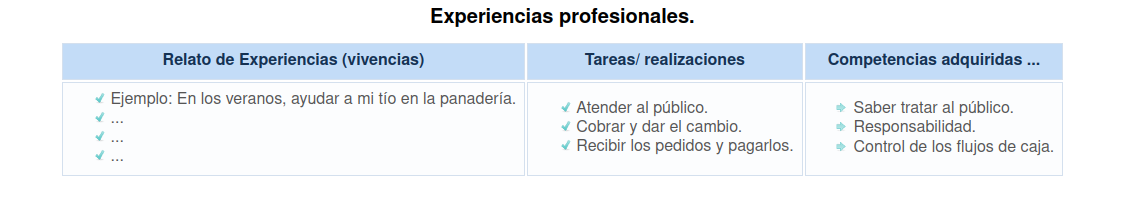
\includegraphics[scale=0.50]{experiencia-prof.png}
        \caption{Proyecto Profesional: Experiencia Profesional}
    \end{figure}

    \item \textbf{Aspecto positivos y negativos de tu personalidad}: indica, en un esquema como el de la siguientes figura, 5 aspectos positivos y negativos de tu personalidad. También puedes pedirle a alguien que te conozca bien que los escriba, para que sean lo mas subjetivos posible.

    \begin{figure}[ht]
        \centering
        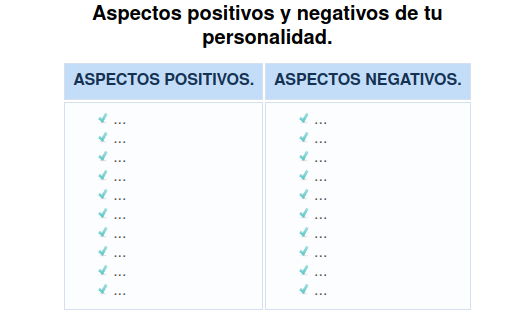
\includegraphics[scale=0.50]{aspectos-pos.png}
        \caption{Proyecto Profesional: Aspectos Personalidad}
    \end{figure}

    \item \textbf{Valores de trabajo que posees}: crea una tabla como la siguiente y rellénala con los valores que posees y que pueden aportarte valor como empleado.

    \begin{figure}[ht]
        \centering
        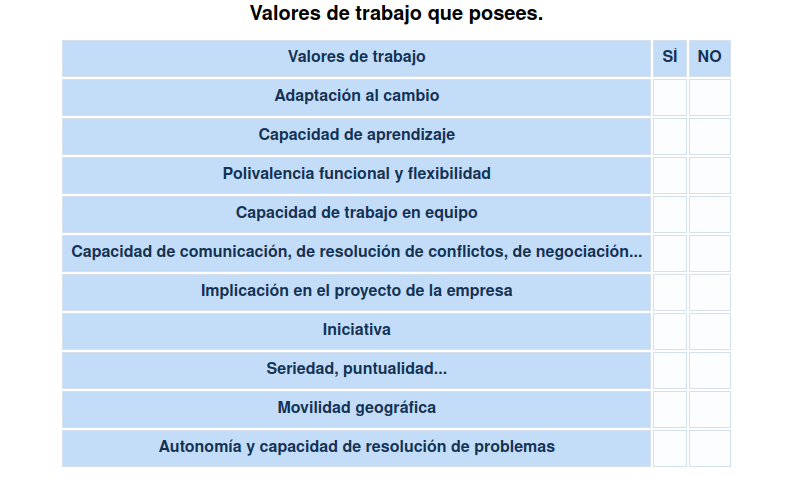
\includegraphics[scale=0.50]{valores-trabajo.png}
        \caption{Proyecto Profesional: Valores de Trabajo}
    \end{figure}
\end{itemize}

\subsection{Analisis de Mercado}
Realiza una búsqueda de ofertas de empleo y rellena un cuestionario como el que se muestra a continuación:

\begin{figure}[ht]
    \centering
    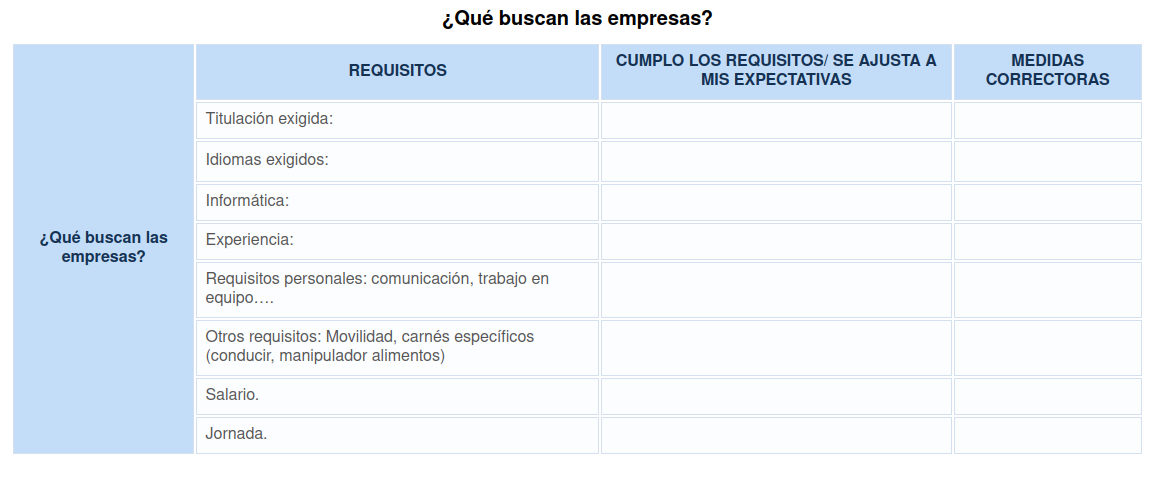
\includegraphics[scale=0.50]{estudio-mercado.png}
    \caption{Proyecto Profesional: Estudio de Mercado}
\end{figure}

\subsection{Objetivo Profesional}
El siguiente paso es definir cual es tu objetivo profesional. Para ello sigue estos pasos:

\begin{itemize}
    \item \textbf{Definir el objetivo}: define cual es tu meta, es decir, que puesto/s te gustaría ocupar.

    \item \textbf{¿Que necesito para conseguir?}: analiza y busca información sobre que \textbf{requisitos} tanto \textbf{formativos} como de \textbf{experiencia} se suelen requerir en ese puesto, elabora una lista con estos requisitos así como otros aspectos que necesites para conseguir tu objetivo.

    \item \textbf{Medidas Correctoras}: a partir de la lista anterior, elabora otra con el conjunto de \textbf{medidas} que vas a adoptar para \textbf{mejorar} aquellos aspectos en los que hayas detectado \textbf{carencias}.

    \item \textbf{Condiciones laborales}: determina las preferencias relativas a las condiciones laborales que esperas así como cuales estás dispuesto a aceptar. Elabora una tabla como la que se muestra en la siguiente figura.
    \begin{figure}[ht]
        \centering
        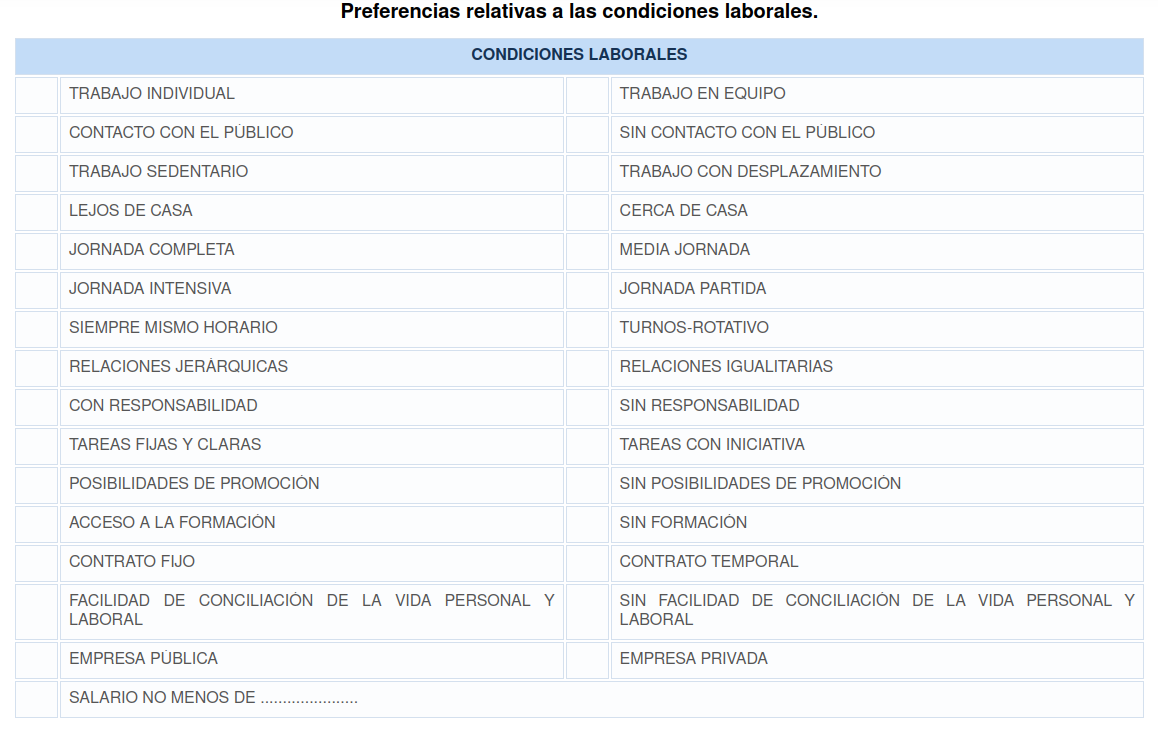
\includegraphics[scale=0.45]{condiciones-laborales.png}
        \caption{Proyecto Profesional: Condiciones Laborales}
    \end{figure}

    \item \textbf{Pasos a Seguir}: elabora una lista con los pasos que deberás seguir para la consecución del objetivo final, que es conseguir un empleo en el puesto deseado.

    \item \textbf{Alternativas}: por si falla el plan, elabora una lista con alternativas.
\end{itemize}

\section{Tipos de Currículum y Estructura}
En este anexo se profundiza más en los tipos de currículum que podemos encontrar en la estructura básica que deber tener cualquier currículum

\subsection{Tipos de Currículum}
Los tipos de currículum mas comunes son los siguientes:

\begin{itemize}
    \item \textbf{Currículum Vitae Cronológico}

    Es el más utilizado es muy buen recibido por los seleccionadores de empleo que buscan estudiar tu personalidad  a través de los mismos. Permite presentar la información de lo mas antiguo a lo más reciente y tiene la \textbf{ventaja} de \textbf{resaltar la evolución} seguida. Tiene el \textbf{inconveniente} de que las \textbf{primeras experiencias} son \textbf{menos relevantes} y las \textbf{lagunas en el tiempo} se \textbf{resaltan más}. Es interesante usar este modelo siempre que:

    \begin{itemize}
        \item Tus puestos de trabajo han evolucionado por orden cronológico y dentro de una misma línea.
        \item Has tenido pocos trabajos y con funciones idénticas o muy similares.
        \item No quieres cambiar la línea de trabajo.
    \end{itemize}

    \item \textbf{Currículum Cronológico Inverso}

    Este modelo de currículum, que gana cada día mas adeptos, consiste en presentar el currículum en orden cronológico pero con los eventos mas recientes en primera instancia. Tiene la \textbf{ventaja} que \textbf{resalta} las \textbf{experiencias más recientes}, que al final son las más importantes.

    \item \textbf{Currículum Vitae Funcional}

    En este modelo se distribuye la información por temas y proporciona un conocimiento rápido de tu experiencia y formación en un ámbito concreto. No sigue un orden cronológico, por lo que permite resaltar los puntos positivos, trabajos y funciones acordes al puesto que solicitas, más que su evolución. También permite omitir los eventuales errores de recorrido, los periodos de paro, frecuentes cambios de trabajo,... Este currículum se escribe pensando en las exigencias de un puesto determinado y dando respuesta a las necesidades de al empresa. Es importante antes de comenzar a redactarlo, tener bien claro los siguientes puntos:

    \begin{itemize}
        \item Tu objetivo ocupacional.
        \item Las experiencias, funciones y logros que se relacionen con tu objetivo profesional.
        \item Empresas en las que hayas realizado funciones requeridas para la consecución de tu objetivo.
        \item La formación académica, así como cursos y seminarios relacionados con tu objetivo.
        \item Este modelo destaca la diferencias que poseer para ocupar un puesto en particular y es \textbf{especialmente útil} cuando tu \textbf{experiencia no esta relacionada} con el puesto al que te estas presentando, cuando estas optando por un \textbf{cambio de carrera profesional}, cuando reingresas al \textbf{mercado laboral} tras un tiempo de paréntesis o cuando estás entrando al mercado laboral por primera vez.
    \end{itemize}
\end{itemize}

\subsection{Estructura del Currículum}
Cualquier currículum debe incluir, como mínimo, los siguientes puntos:

\begin{enumerate}
    \item \textbf{Datos Personales}: nombre y apellidos, lugar de nacimiento, nacionalidad (si no es española), dirección personal, teléfono de contacto y correo electrónico.

    \item \textbf{Formación Académica}: estudios reglados realizados relativos al perfil solicitado por la empresa, indicando el centro y la localidad de realización y fechas. Se deben incluir solo los estudios de más alto nivel, no siendo necesario incluir la educación secundaria. Tampoco se debe hacer referencia a las calificaciones obtenidas.

    \item \textbf{Formación Complementaria}: estudios no reglados como cursos o seminarios, indicando centro y horas lectivas, que sean relativos al puesto que se quiere ocupar.

    \item \textbf{Idiomas}: conocimientos de idiomas precisando el nivel oral y escrito. Si obtuviste algún título reconocido o tuviste alguna estancia en el extranjero indícalo.

    \item \textbf{Informática}: conocimientos de informática especificando el grado de domino de programas, aplicaciones y lenguajes de programación.

    \item \textbf{Experiencia Profesional}: relación de la diferentes experiencias profesionales realizadas. Es imprescindible dar el máximo detalle posible: nombre y actividad de la empresa, fechas, puestos y funciones desempeñadas. Esto permitirá a la persona que lea tu currículum evaluar rápidamente las competencias. En caso de no tener experiencia incluye las prácticas que hayas realizado durante tus estudios y las actividades de voluntariado.

    \item \textbf{Datos de Interés}: datos no incluidos en los apartados anteriores, pero solo aquellos que aporten información relevante sobre tu perfil y puedan aumentar el valor de tu currículum: premios literarios, carnet de conducir, vehículo propio, disponibilidad para viajar, etc..
\end{enumerate}

\section{Tipos de Relaciones con la Administración}
Los tipos de relaciones que se pueden establecer con las Administración Pública son los siguientes:

\begin{itemize}
    \item \textbf{Funcionario de Carrera}: personal de plantilla de la Administración Pública que presta sus servicios de forma permanente. Se trata de relaciones reguladas por el Derecho Administrativo.

    \item \textbf{Funcionario Interino}: son personal funcionario de empleo interino quienes, por razones expresamente justificadas de necesidad y urgencia, son nombrados como tales para el desempeño de las labores de los funcionarios de carrera, cuando se de alguna de las siguientes circunstancias:

    \begin{itemize}
        \item La existencia de plazas vacantes cuando no sea posible su cobertura por funcionarios de carrera.
        \item La sustitución transitoria de las personas titulares de la plaza.
        \item La ejecución de programas de carácter temporal.
        \item El exceso o acumulación de tareas por plazo máximo de 6 meses dentro de un período de 12 meses.
    \end{itemize}

    \item \textbf{Personal Laboral}: son aquellos trabajadores asalariados contratados por la Administración Pública, cuya relación es regulada por el Derecho Administrativo y los convenios colectivos. Sus contratos pueden ser indefinidos o de duración limitada. Las categorías profesionales de estos trabajadores son las que fijan los convenios y se fijan en función de la titulación exigida para la convocatoria.

    \item \textbf{Personal Eventual}: son quienes, en virtud de nombramiento y con carácter no permanente, solo realizan funciones expresamente calificadas como de confianza o asesoramiento especial, retribuyéndoseles con cargo a los presupuestos consignados a este fin.
\end{itemize}

\section{Formas de Acceso a Empleo Público}
Las formas de acceso al empleo pública son las siguientes:

\begin{itemize}
    \item \textbf{Contratación temporal bajo presupuesto de programas específicos}: las entidades públicas pueden solicitar programas que incluyan la contratación de personal. Hay que tener en cuenta que estos contratos duran exclusivamente lo que dura el programa, y no hay obligatoriedad de vinculación posterior con la entidad.

    \item \textbf{Bolsas de trabajo por concurso de méritos}: las Administraciones pueden hacer pública una necesidad de personal, haciendo una baremación de méritos (títulos, cursos realizados, experiencia laboral).

    \item \textbf{Oposiciones}: una oposición es un procedimiento selectivo consistente en una o más pruebas elaboradas sobre un temario oficial, en que los aspirantes a un puesto de trabajo muestran sus respectivas competencias, juzgadas por un tribunal. Estas pruebas suelen ser duras, debes de tener claro que quieres preparártelas antes de hacer la inversión de tiempo y esfuerzo. También debes considerar que muchas oposiciones comparten parte del temario, así que con un poco de esfuerzo extra puedes presentarte a distintas plazas. Lo mejor es considerar esta opción como un objetivo a conseguir a medio y largo plazo. Estos puestos de trabajo son ofrecidos a través de convocatorias por las Administraciones Públicas, de ahí que estas ofertas de empleo se denominen Ofertas de Empleo Público (OPE), publicadas en los Boletines Oficiales del Estado, Autonomías y Provincias.

    En muchas de ellas, las convocatorias establecen la posibilidad de crear listas de interinidades/bolsas de trabajo con aquellos aspirantes que no hayan obtenido plaza o no hayan superado el proceso selectivo, de tal forma que cuando se precise personal para cubrir una incapacidad temporal de un titular o por existir una vacante, se llamará a las personas de esa bolsa.

    \item \textbf{Concurso-Oposición}: Al igual que en la oposición consiste en pruebas selectivas elaboradas sobre un temario oficial, no obstante en este caso la calificación final vendrá determinada no sólo por la nota del examen o prueba de conocimientos, sino también por los méritos.
\end{itemize}

Los méritos vendrán determinados por experiencia en puestos de la misma categoría a la que se opta, titulaciones oficiales y los denominados ``\textbf{cursos baremables}''. Fíjate bien en ellos, porque estos cursos te pueden dar la llave al empleo, ya que otorgan puntos para la oposición. Son cursos aceptados por las diversas Administraciones en sus convocatorias de Empleo Público y en las diversas bolsas de trabajo. Son impartidos por sindicatos, organizaciones empresariales, Comunidades Autónomas... Lee bien la convocatoria e infórmate en el organismo que las convoca qué cursos son baremables y dónde los puedes realizar. Por último al igual que en las oposiciones es habitual que en esta forma de acceso la convocatoria establezca la creación de listas de interinidades/ bolsas de trabajo o sustituciones.


% Glossary
\glsaddall
\printglossaries

% Bibliography
\newpage
\addcontentsline{toc}{chapter}{Bibliografía}
\bibliography{citas}
\bibliographystyle{unsrt}

\end{document}